%                                                                 aa.dem
% AA vers. 9.1, LaTeX class for Astronomy & Astrophysics
% demonstration file
%                                                       (c) EDP Sciences
%-----------------------------------------------------------------------
%
%\documentclass[referee]{aa} % for a referee version
%\documentclass[onecolumn]{aa} % for a paper on 1 column  
%\documentclass[longauth]{aa} % for the long lists of affiliations 
%\documentclass[letter]{aa} % for the letters 
%\documentclass[bibyear]{aa} % if the references are not structured 
%                              according to the author-year natbib style

%
\documentclass[draft]{aa}
% \documentclass{aa}
% \documentclass[referee]{aa}

%
\usepackage{graphicx}
%%%%%%%%%%%%%%%%%%%%%%%%%%%%%%%%%%%%%%%%
\usepackage{txfonts}
%%%%%%%%%%%%%%%%%%%%%%%%%%%%%%%%%%%%%%%%
%\usepackage[options]{hyperref}
% To add links in your PDF file, use the package "hyperref"
% with options according to your LaTeX or PDFLaTeX drivers.
%
\usepackage[]{hyperref}
\hypersetup{colorlinks=true, urlcolor=blue, citecolor=cyan, pdfborder={0 0 0}}

% \usepackage{natbib}

% Ignore Appendix
% \renewcommand\appendix{\end{document}}

% "Fix" hyperlink spilling out of page error
% \hypersetup{draft}
%\usepackage{amstext}

\begin{document}

\title{Sixteen overlooked open clusters in the fourth Galactic quadrant}
\subtitle{A combined analysis of UBVI photometry and Gaia DR2 with 
\texttt{ASteCA}\thanks{
Photometric tables are available in electronic form
at the CDS via anonymous ftp to cdsarc.u-strasbg.fr (\url{130.79.128.5})
or via \url{http://cdsweb.u-strasbg.fr/cgi-bin/qcat?J/A+A/}}}

\author{G. I. Perren\inst{1}
      \and
      E. E. Giorgi\inst{2}
      \and
      A. Moitinho\inst{3}
      \and
      G. Carraro\inst{4}
      \and
      M. S. Pera\inst{1}
      \and
      R. A. Vázquez\inst{2}
      % \fnmsep\thanks{Just to show the usage
      % of the elements in the author field}
}

\institute{Instituto de Astrof\'isica de La Plata (IALP-CONICET), La Plata,
Argentina\\
\email{gabrielperren@gmail.com}
\and
Facultad de Ciencias Astronómicas y Geofísicas (UNLP-IALP-CONICET), 1900 La
Plata, Argentina
\and
CENTRA, Faculdade de Ci\^encias, Universidade de Lisboa, Ed. C8, Campo Grande,
1749-016 Lisboa, Portugal
% SIM, Faculdade de Ciências, Universidade de Lisboa, Ed. C8, Campo Grande,
% P-1749-016 Lisboa, Portugal
\and
Dipartimento di Fisica Astronomia Galileo Galilei, Vicolo Osservatorio 3,
Padova, I-35122, Italy
% \thanks{The university of heaven temporarily does not
%         accept e-mails}
}

\date{Received November xx, 2019; accepted xxxx xx, 2019}


\abstract
% 5 {} token are mandatory
% context heading (optional)
{}
% aims heading (mandatory)
{This paper has two main objectives:
(1) To determine the intrinsic properties of 16 faint and mostly
unstudied open clusters in the poorly known sector
of the Galaxy at $270^\circ-300^\circ$ to probe the Milky Way
structure in future investigations.
(2) To address previously reported systematics in Gaia DR2 parallaxes by
comparing the cluster distances derived from photometry with
those derived from parallaxes.
}
%
% methods heading (mandatory)
{Deep \textit{UBVI} photometry of 16 open clusters was carried out.
Observations were reduced and analyzed in an automatic way using the 
\texttt{ASteCA} package to obtain individual distances, reddening,
masses, ages, and metallicities. Photometric distances were compared to
those obtained from a Bayesian analysis of Gaia DR2 parallaxes.
}
%
% results heading (mandatory)
{Ten out of the sixteen clusters are true or highly probable open
clusters. Two of them are quite young and follow the trace of the Carina Arm
and the already detected warp.
The remaining clusters are placed in the interarm zone between the
Perseus and Carina Arms, as expected for older objects.
We found that the cluster van den Berg-Hagen 85 is $7.5\times10^9$ yr
old, which means that it is one of the oldest open clusters detected in our
Galaxy so far.
%
The relationship of these ten clusters with the Galaxy structure in
the solar neighborhood is discussed.
The comparison of distances from photometry and parallaxes data in turn
reveals a variable level of disagreement.
}
%
% conclusions heading (optional), leave it empty if necessary
{
Various zero-point corrections for Gaia DR2 parallax data recently
reported were considered for a comparison between photometry- and
parallax-based distances.
The results tend to improve with some of these corrections. 
Photometric distance analysis suggests an average correction of
$\sim$+0.026 mas (to be added to the parallaxes).
%
The correction may have a more intricate dependence on distance, but addressing
this level of detail will require a larger cluster sample.
}

\keywords{
  Methods: statistical --
  Galaxies: star clusters: general --
  (Galaxy:) open clusters and associations: general --
  Techniques: photometric--
  Parallaxes --
  Proper motions
}

\maketitle




%================================================================
\section{Introduction}

Galactic open clusters are routinely used as probes of the structure and
evolution of the Milky Way disk. Their fundamental parameters, such as age,
distance, and metallicity, allow us to define the large-scale structure of the
disk and to cast light on its origin and assembly \citep{Janes_1982,
Moitinho_2010,2018A&A...618A..93C}. Young open clusters can be used to trace
spiral arms and star-forming regions \citep{Moitinho_2006,Vazquez2008}, while
older clusters are better probes of the chemical evolution of the thin disk
\citep{2009yCat..35120063M}. The recent second release of Gaia satellite data
\citep{GaiaDR2_2018} is producing a tremendous advance in the study of the
Galactic disk and its stellar cluster population.

Basic parameters for a large number of clusters are now available with
unprecedented accuracy \citep{2018A&A...618A..93C,Soubiran_2018,Bossini_2019,
Monteiro_2019}. Proper motions may be employed to select cluster members, and
parallaxes can be used to derive distances. However, in some cases, Gaia
parallax distances disagree with the distances derived from other methods 
(i.e., photometric or spectrophotometric). It may occur that the photometric and parallax distances yield similar results
within the uncertainties for short distances \citep{2018A&A...618A..93C}. The
situation is complex regarding the existence of a bias correction to be applied
to Gaia parallaxes, however. The analysis of quasar measurements in Gaia DR2 by
\cite{Lindegren_2018} led to the determination of a global zero-point
correction to parallaxes of approximately 0.03 mas, with variations of a
comparable size depending on magnitude, color, and position.
More recently, by analyzing a sample of stars, \cite{Schonrich2019} have shown
that not only must a parallax offset be applied to Gaia data, but a
quasi-linear dependence exists with distances.
\cite{Xu_2019}, who compared distances of a variety of astronomical objects
between Gaia and very long baseline interferometry (VLBI) parallaxes, also
reported a zero-point parallax correction of $\sim$0.075 mas.
It is difficult to establish the critical distance at which Gaia parallax
distances begin to diverge from values based on other methods and the dependence of
the bias on position, parallax, or other measurements. The  task of
establishing distances and other essential parameters for open clusters using
the Gaia data appears to be arduous because other factors such as interstellar
absorption and the level of crowding of a given stellar cluster also play a
role.

In this article we present a sample of 16 cataloged stellar clusters
\citep{Dias_2002} that have not been studied previously and are located in a
poorly known Galactic sector at approximately $270^\circ<l<300^\circ$ in the
Galactic plane. With one exception, this is the first systematic study carried
out for the clusters in our sample. In this
sense, we provide CCD \textit{UBVI} photometry complemented with data available
from Gaia DR2. The purpose of this investigation is twofold. First, we search
for a reliable estimation of the true nature of these objects. Gaia DR2 offers
us a long-sought opportunity because we can make our analysis more reliable by
combining  ground-based \textit{UBVI} CCD data with space-based astrometry 
(parallax and proper motions) and photometry. Second, because distance is the
main derived parameter for mapping the Galaxy’s structure, we seek to
understand and take
into account the corresponding biases in Gaia DR2 parallaxes.
In following studies, we investigate the structure of the
Galactic disk in this region. Traces of the Perseus Arm coming from of the
third Galactic quadrant  are expected, although this arm is only
prominent in the second quadrant. However, we recall 
that some of these clusters may be associated with the Carina Arm.

It has proved to be quite challenging to analyze this sector of the Galaxy because the extinction is particularly strong and variable. This
makes it not only difficult to derive accurate basic parameters of a cluster,
but even worse, it is hard to establish whether a visual stellar aggregate is a physical
cluster or simply a random enhancement of field stars produced by patchy
extinction. 
%
To achieve these two purposes, we employed the \textbf{Automated Stellar
Cluster Analysis} code \citep[\texttt{ASteCA};][]{Perren_2015} to derive
the fundamental cluster parameters from \textit{G-UBVI} data, and two Bayesian
techniques to extract membership probabilities and distances from Gaia DR2. The
sample of clusters studied in this paper is shown in Table 
\ref{tab:clust_list} together with their Galactic coordinates and their
equatorial coordinates referred to the J2000.0 equinox.

The paper is \textbf{structured} as follows: in Section \ref{sec:clust_sample} we
present the cluster sample.
Section \ref{sec:photo_obs} is devoted to explaining the observations and the
reduction process of photometry. In Section \ref{sec:photom_analysis} we
describe the tools we used to analyze the photometric data and the method with which we connect
Gaia DR2 with photometric results. A cluster-by-cluster report of the results
obtained is presented in Section \ref{sec:cluster_discuss}. In Section
\ref{sec:gaia_distances} three different corrections to Gaia DR2 parallax
data are applied and discussed. Our conclusions are given in Section 
\ref{sec:results_concl}.




%================================================================
\section{Cluster sample}
\label{sec:clust_sample}

Table \ref{tab:clust_list} lists the equatorial coordinates ($\alpha$,
$\delta$) and Galactic coordinates (\textit{l}, \textit{b}) of the 16 cluster
fields studied here, ordered by increasing right ascension $\alpha$.
Equatorial coordinates refer to the J2000.0 equinox.

\begin{table}[ht]
    \centering
\caption{List of objects. Note: van den
Bergh-Hagen clusters \citep{vdBH1975} are indicated by vdBH. In a similar   
way, Ruprecht \citep{Ruprecht_1996} and Trumpler \citep{Trumpler_1930} clusters
listed as RUP and TR followed by the respective numbers.}
    \begin{tabular}{lcccc}
    \hline \hline 
        Cluster name & $\alpha_{2000}$ & $\delta_{2000}$ & \emph{l} & \emph{b}\\
         & hh:mm:ss & dd:mm:ss & $^\circ$ & $^\circ$\\
       \hline
        vdBH 73 & 09:31:56 & -50:13:00 & 273.634 & 0.951\\
        vdBH 85 & 10:01:52 & -49:34:00 & 276.914 & 4.544\\
        RUP 87 & 10:15:32 & -50:43:00 & 279.372 & 4.883\\
        RUP 85 & 10:01:33 & -55:01:12 & 280.15 & 0.160\\
        vdBH 87 & 10:04:18 & -55:26:00 & 280.719 & 0.059\\
        vdHB 92 & 10:19:07 & -56:25:00 & 282.984 & 0.438\\
        TR 12 & 10:06:29 & -60:18:00 & 283.828 & -3.698\\
        vdBH 91 & 10:17:16 & -58:42:00 & 284.03 & -1.600\\
        TR 13 & 10:23:48 & -60:08:00 & 285.515 & -2.353\\
        vdBH 106 & 10:52:42 & -54:14:00 & 286.048 & 4.700\\
        RUP 88 & 10:18:55 & -63:08:00 & 286.661 & -5.186\\
        RUP 162 & 10:52:54 & -62:19:00 & 289.638 & -2.545\\
        Lynga 15 & 11:42:24 & -62:29:00 & 295.053 & -0.672\\
        Loden 565 & 12:08:06 & -60:43:12 & 297.65 & 1.710\\
        NGC 4230 & 12:17:20 & -55:06:06 & 298.025 & 7.445\\
        NGC 4349 & 12:24:08 & -61:52:18 & 299.719 & 0.830\\
        \hline
    \end{tabular}
    \label{tab:clust_list}
\end{table}


These objects form part of a long-term joint effort to study the
complicated structure of the Galaxy in the solar neighborhood. With this
motivation, we have been collecting and producing
homogeneous $UBVI$ observations of open clusters in the third Galactic quadrant
(3GQ: $180^\circ\leq l \leq270^\circ$) of the Milky Way during the past decade.
We understand that for a better interpretation of the galaxy structure from an
optical point of view, \textbf{it is essential} to increase the number of these  objects
with well-estimated parameters. We have contributed significantly to the
current understanding of the spiral structure in this Galactic region
\citep{Carraro_2005,Moitinho_2006,Vazquez2008,Carraro_2010}.
In this article we focus on unknown open clusters that are placed
between the end of the 3GQ and 300 in Galactic longitude for a similar
purpose.

The positions of the clusters in the Galaxy are shown in Fig. \ref{fig1}, superposed
onto the Aladin Sky Atlas DSS2 color image. Our sampling essentially covers the
first 30 degrees of the fourth Galactic quadrant, from latitudes
$l\sim$273$^\circ$ to $l\sim$300$^\circ$, encompassing the region around the
Carina OB association and the southeast part of Vela, with some objects in Crux
and Centaurus.


\begin{figure*}[ht]
    \centering
    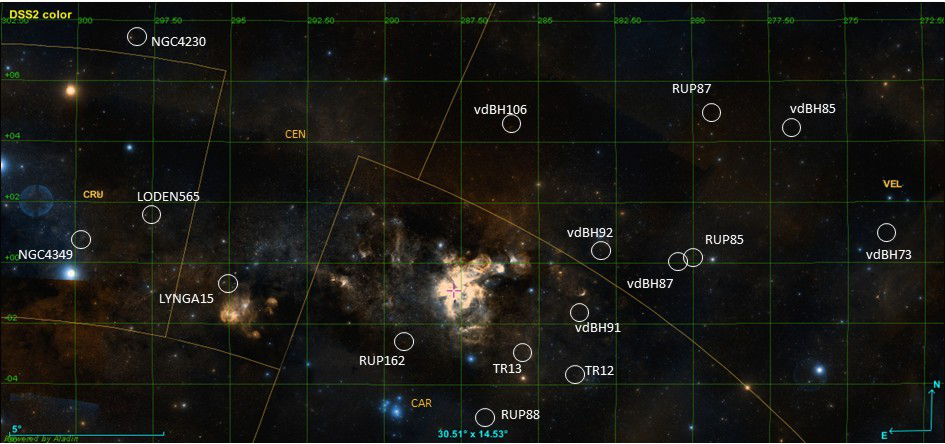
\includegraphics[width=\hsize]{../figs/DSS2color.png}
    \caption{Aladin DSS2 color image showing with white circles the positions of
    the clusters we survey here. The Galactic coordinates $l$
    and $b$ are depicted by a green grid, and constellation limits for Carina,
    Vela, Centaurus, and Crux are plotted as yellow lines.}
    \label{fig1}
\end{figure*}




%================================================================
\section{Photometric observations}
\label{sec:photo_obs}

A first series of CCD \emph{UBVI} photometry was carried out on 13 open clusters
placed in the Galactic region that extends from 270$^\circ$ to 300$^\circ$ in Galactic
longitude and from 7$^\circ$ to -5$^\circ$ in Galactic latitude. This region
covers the Carina Arm, the interarm region between the Perseus and Carina arms,
and also a part of the Local Arm.
%
The observations were made on nine nights in April and May 2002, using the YALO
(Yale, AURA, Lisbon, OSU)
\footnote{http://www.astronomy.ohio-state.edu/YALO/}
facilities at Cerro Tololo Inter-American
Observatory (CTIO). The images were taken with a $2048\times2048$ px CCD
attached to the 1.0 m telescope and the set of \textit{UBVI} filters.
The field of view is $10^\prime\times10^\prime$ given the
$0.3^{\prime\prime}$/px plate scale. All images were acquired using the
ANDICAM\footnote{\url{http://www.astronomy.ohio-state.edu/~depoy/research/instrumentation/andicam/andicam.html}},
which was moved to the 1.3 m CTIO telescope in 2003.

A second series of CCD photometry was implemented during March 2010 at CTIO
to obtain \textit{UBVI} photometry in two other clusters,
NGC 4349 and Lynga 15; they lie at a slightly higher Galactic longitude 
(298$^\circ$). Images in a first run were taken with the
SMARTS 0.9 m telescope\footnote{
\url{http://www.ctio.noao.edu/noao/content/SMARTS-09-m-Telescope}}
using a $2048\times2046$ px Tek2K
detector\footnote{\url{http://www.ctio.noao.edu/noao/content/Tek2K}} with a
scale $0.401^{\prime\prime}$/px, covering thus $13.6^{\prime}$ on a side. A
second run of images taken at the SMARTS 1.0 m telescope\footnote{
\url{http://www.ctio.noao.edu/noao/content/SMARTS-10-m-Telescope}}
of the same clusters was carried out with a $4064\times4064$ px
Y4KCam\footnote{\url{http://www.ctio.noao.edu/noao/content/y4kcam}}
CCD with a scale of $0.289^{\prime\prime}$/px, thus covering
$20^\prime\times20^\prime$ on a side.
%
The first run (at the 0.9 m) was not photometric, and therefore we tied all
the images to the second run (at the 1.0 m), which was photometric. During
this second run, we took multiple images of the standard star fields PG 1047
and SA98 \citep{1992AJ....104..340L}.

Finally, in 2015, the open cluster vdBH 73, located at a lower
longitude ($\sim 273^\circ$), was observed in the \textit{UBVI} filters with the
1.0 m Swope telescope\footnote{\url{http://www.lco.cl/telescopes-information/henrietta-swope/telescope-control-system/telescopes-information/henrietta-swope/instruments/}}
at Las Campanas Observatory, Chile. On this occasion,
direct images were acquired with the 4kx4k E2V CCD with a scale of
$0.435^{\prime\prime}$/px, covering $29.7^\prime\times29.8^\prime$.\\

Short exposures were always obtained to avoid bright star saturation in the
frame.\textbf{ Notwithstanding, very bright stars are sometimes lost}.
Details of air masses, seeing values, and exposure times per filter and
telescope are listed in Table \ref{tab:log_yalo} for all the observations.

% seeing [''] = FWHM * scale [''/px]
% vdBH73: scale = 0.435 ''/px

\begin{table*}[ht]
    \centering
    \caption{Log of observations at YALO (CTIO) and Las Campanas.
    References for the telescopes are 1 (1.0 m YALO), 2 (0.9 m, 1.0 m SMARTS), and
    3 (1.0 m Swope). Air masses and seeing are averaged values for the short and
    long exposures.}
    \begin{tabular}{lcccccc}
    \hline \hline 
        Cluster & Date & Telescope & U & B & V &  I\\
                &      &           &
        \multicolumn{4}{c}{(airmass, seeing [''], short exp/long exp [sec])}\\
       \hline
        vdBH 73   & 06/2015 & 3 & 1.2, 2.8, 50/150 & 1.2, 2.8, 20/60 &
        1.17, 2.0, 15/45  & 1.16, 2.43, 15/45\\
        vdBH 85   & 04/2002 & 1 & 1.09, 1.7, 30/300 & 1.07, 1.7, 5/200 &
        1.07, 1.5, 3/160 & 1.14, 1.6, 1/120\\
        RUP 87    & 04/2002 & 1 & 1.14, 1.9, 30/300 & 1.11, 1.7, 5/200 &
        1.09, 2.0, 3/160 & 1.07, 1.6, 1/120\\
        RUP 85    & 04/2002 & 1 & 1.11, 2.5, 30/300 & 1.11, 2.1, 5/200 &
        1.11, 1.9, 3/160 & 1.13, 1.7, 1/120\\
        vdBH 87   & 04/2002 & 1 & 1.11, 2.2, 30/300 & 1.11, 2.5, 5/200 &
        1.12, 2.0, 3/160 & 1.14, 1.7, 1/120\\
        vdBH 92   & 05/2002 & 1 & 1.12, 1.9, 60/300 & 1.12, 1.9, 20/200 &
        1.12, 2.0, 10/160 & 1.12, 1.8, 10/120\\
        TR 12     & 04/2002 & 1 & 1.19, 1.7, 30/300 & 1.17, 1.8, 5/200 &
        1.16, 1.6, 3/160 & 1.16, 1.5, 1/120\\
        vdBH 91   & 05/2002 & 1 & 1.14, 2.1, 60/300 & 1.14, 2.0, 20/200 &
        1.15, 2.0, 10/160 & 1.17, 1.8, 10/120\\
        TR 13     & 05/2002 & 1 & 1.17, 1.8, 60/300 & 1.16, 1.6, 20/200 &
        1.16, 1.6, 10/160 & 1.16, 1.4, 10/120\\
        vdBH 106  & 05/2002 & 1 & 1.10, 2.3, 60/300 & 1.11, 2.3, 20/200 &
        1.13, 2.1, 10/160 & 1.15, 2.1, 10/120\\
        RUP 88    & 05/2002 & 1 & 1.19, 2.2, 60/300 & 1.19, 2.1, 20/200 &
        1.2, 2.0, 10/160 & 1.21, 1.8, 10/120\\
        RUP 162   & 05/2002 & 1 & 1.18, 1.6, 60/300 & 1.19, 1.6, 20/200 &
        1.0, 1.5, 10/160 & 1.2, 1.4, 10/120\\
        Lynga 15  & 03/2010 & 2 & 1.19, 1.9, 5/2400 & 1.25, 1.9, 3/1800 &
        1.28, 1.19, 3/1100 & 1.27, 1.19, 3/1100\\
        Loden 565 & 05/2002 & 1 & 1.16, 1.9, 60/300 & 1.17, 1.7, 20/200 &
        1.17, 1.7, 10/160 & 1.19, 1.6, 10/120\\
        NGC 4230  & 05/2002 & 1 & 1.11, 2.1, 60/300 & 1.12, 1.8, 20/200 &
        1.13, 1.8, 10/160 & 1.16, 1.6, 10/120\\
        NGC 4349  & 03/2010 & 2 & 1.18, 1.8, 5/2400 & 1.18, 1.6, 3/1800 &
        1.18, 1.5, 3/1100 & 1.18, 1.4, 3/1100\\
        \hline
    \end{tabular}
    \label{tab:log_yalo}
\end{table*}




% ------------------------------------------------------------------
\subsection{Photometric reduction process}
\label{ssec:photom_reduc}

The basic reduction of the CCD science frames was made in the standard way
using the IRAF 4 package \texttt{ccdred}. Photometry was performed using
the IRAF DAOPHOT \citep{Stetson_1987,Stetson_1990} and \texttt{photcal} packages.
Aperture photometry was performed to obtain the instrumental magnitudes of
standard stars and some bright cluster stars. Profile-fitting photometry was
performed in each program frame by constructing the corresponding point spread
function. The zero-point of the instrumental magnitudes for each image was
determined with aperture photometry and growth curves.

The transformation equations to convert instrumental magnitudes into the
standard system were always of the form

\begin{equation}
\begin{aligned}
  u  &=  U+u_1+u_2xX+u_3x(U-B), \\
  b  &=  B+b_1+b_2xX+b_3x(B-V), \\
  v  &=  V+v_1+v_2xX+v_3x(B-V), \\
  i  &=  I+i_1+i_2xX+i_3x(V-I),
\end{aligned}
\end{equation}


\noindent where $u_2, b_2, v_2,\text{ and } i_2$ are the extinction coefficients computed
for each night, and $X$ is the air-mass. No color dependence of higher
order was found for either filter.

In each case, detector coordinates were cross-matched with Gaia astrometry to
convert pixels into equatorial $\alpha$ and $\delta$ for the equinox J2000.0,
thus providing Gaia-based positions for the entire cluster catalog.
This process was performed in three steps. First, the
Astrometry.net\footnote{\url{http://astrometry.net/}} service was used to
assign ($\alpha$, $\delta$) coordinates to the brightest stars in our observed
frames. The second step involved employing our own code, called 
\texttt{astrometry}\footnote{\url{https://github.com/Gabriel-p/astrometry}} , to
apply a transformation from pixel to equatorial coordinates to all the observed
stars, using the coordinates already assigned to the brightest stars matched in
the previous step. The algorithm in this code applies the affine transformation
method developed by
J. Elonen\footnote{\url{https://elonen.iki.fi/code/misc-notes/affine-fit/}}
based on the work by \cite{Spath2004}. The transformation equations are of
the form $\alpha=c_0+c_1x+c_2y,$ where $\alpha$ is the right ascension,
$(x, y)$ are the pixel coordinates, and the $c_X$ coefficients are fit
(similarly for $\delta$, more details \textbf{on the code site}).
Finally, in the third step, we used another one of our open-source codes, called
\texttt{CatalogMatch}\footnote{\url{https://github.com/Gabriel-p/catalog_match}}
, to cross-match our frames (which by now had equatorial coordinates assigned)
with Gaia DR2\footnote{\url{https://www.cosmos.esa.int/web/gaia/dr2}} data. The
matching tolerance used here ranged from 2 to 4 arcsec, with mean
minimum and maximum differences in the matches of 0.3 and 0.9 arcsec,
respectively (for all the observed frames).\\


With the exception of cluster NGC 4349, the remaining objects in our
sample have no dedicated photometric studies. We were still able to perform
a comparison of our photometry in $V$, $B$, and $(B-V)$ with available
photometry from APASS DR10 (The AAVSO Photometric All-Sky
Survey\footnote{\url{https://www.aavso.org/apass}}), which has a
magnitude limit near 18 mag (enough to identify the presence of red giant branch, RGB, stars), and
Gaia DR2.
%
In this comparison we placed particular emphasis on the clusters belonging to the
observing runs in 2002 because they are mostly very faint.


For APASS data, we downloaded a region centered on each
observed frame and cross-matched it with our data, taking care to remove
bad matches by enforcing a tolerance of 0.7 arcsec on the matches for all the
frames (this value was selected because it gave a reasonable number of
matches with a minimum of bad-match contamination).
%
We also compared our photometry with that from Gaia DR2 using the
Carrasco photometric
relationships\footnote{\url{https://gea.esac.esa.int/archive/documentation/GDR2/Data_processing/chap_cu5pho/sec_cu5pho_calibr/ssec_cu5pho_PhotTransf.html}}
between the Johnson-Cousins system and Gaia passbands. The process
requires transforming the $G$ magnitude into $V$ and $B$ magnitudes through the
transformation equations provided there. For the $V$ filter we employed the
$(G-V)$ versus ($BP-RP$) polynomial. For the $B$ filter, no similar
polynomial has been presented, therefore we fit our own using the same list of
cross-matched Landolt standards as was used by Carrasco.\footnote{This list was kindly
provided by Carrasco upon our request. We thank Dr Carrasco very much for
sharing this data.} This third-degree polynomial is

\begin{equation}
\begin{aligned}
G - B = {} & 0.003[0.009]-0.64[0.02]\,(BP-RP)- \\
        & 0.42[0.03]\,(BP-RP)^2+0.067[0.007]\,(BP-RP)^3
\end{aligned}
,\end{equation}

\noindent
where the values in brackets are the standard deviations of each
coefficient, and the RMS of the residuals is $\sigma\sim0.066$.
As a result of applying these two polynomials, we obtain transformed $G$
magnitude values into $V_{Gaia}$ and $B_{Gaia}$ magnitudes, which we can use for a direct
comparison with our own $V$ and $B$ magnitudes.

The results are shown in Table \ref{tab:phot_diffs}, where the $\Delta V$,
$\Delta B$ and $\Delta (B-V)$ columns display the mean differences
between our photometry and APASS DR10 and Gaia DR2 data for all the observed
regions.
%
In each frame the groups of stars to compare were selected according
to the filter criteria imposed by Carrasco: $G<13$, $\sigma_{G}<0.01$.
%
The mean differences for $V$, $B$ and $(B-V)$ combining all
the frames are shown in Fig \ref{fig:gaia_transf}. Although there are no
visible trends, there are offsets in the $V$ and $B$ magnitudes between our
photometry and APASS of ($\Delta V=-0.07\pm0.07$, $\Delta B=0.06\pm0.08$) and
between our photometry and Gaia of ($\Delta V=-0.03\pm0.04$,
$\Delta B=-0.01\pm0.08$).
%
The reason for the differences found for the offsets between our data and
APASS/Gaia is that APASS DR10 itself is offset from Gaia
DR2 by ($\Delta V=0.04\pm0.07$, $\Delta B=0.05\pm0.10$), in the sense (Gaia -
APASS).
These values were found by directly cross-matching APASS data (for the regions where
our 16 frames are located) with Gaia data, and applying the
transformations for the $G$ magnitude into $V,B$.
%
In any case, these offsets are not relevant because we only use the $(B-V)$
color in the analysis so that the offsets tend to compensate \textbf{for each} other
and result in a lower value of $\sim$0.015 mag.
The effect of this $(B-V)$ offset in our photometry on the estimated
photometric distances is addressed in Sect~\ref{sec:gaia_distances}.\\

\begin{table*}[ht]
    \centering
\caption{Mean differences between APASS and the Carrasco transformation
polynomials and our own photometry. The columns named N show the
number of stars that were used to estimate these values for each cluster.}
    \begin{tabular}{lcccc|cccc}
    \hline \hline 
Cluster & \multicolumn{3}{c}{APASS} & \multicolumn{4}{c}{Gaia}\\
 & $\Delta V$ & $\Delta B$ & $\Delta (B-V)$ & N & $\Delta V$ &
$\Delta B$ & $\Delta (B-V)$ & N\\
    \hline
vdBH 73   & -0.07$\pm$0.05 & -0.04$\pm$0.05 & 0.03$\pm$0.03 & 301 &
-0.03$\pm$0.03 & -0.01$\pm$0.07 & 0.01$\pm$0.07 & 95\\
vdBH 85   & 0.01$\pm$0.04 & 0.03$\pm$0.05 & 0.03$\pm$0.04 & 32 &
0.01$\pm$0.02 & 0.02$\pm$0.07 & 0.00$\pm$0.07 & 11\\
RUP 87    & -0.02$\pm$0.05 & 0.01$\pm$0.09 & 0.02$\pm$0.07 & 41 &
0.00$\pm$0.02 & 0.00$\pm$0.03 & 0.00$\pm$0.04 & 17\\
RUP 85    & -0.04$\pm$0.05 & -0.02$\pm$0.10 & 0.02$\pm$0.08 & 36 &
-0.01$\pm$0.02 & 0.02$\pm$0.03 & 0.03$\pm$0.03 & 22\\
vdBH 87   & -0.03$\pm$0.05 & -0.02$\pm$0.06 & 0.01$\pm$0.04 & 37 &
-0.02$\pm$0.03 & 0.02$\pm$0.06 & 0.04$\pm$0.08 & 18\\
vdBH 92   & -0.06$\pm$0.05 & -0.05$\pm$0.06 & 0.01$\pm$0.04 & 34 &
-0.02$\pm$0.04 & 0.02$\pm$0.07 & 0.03$\pm$0.04 & 20\\
TR 12     & -0.07$\pm$0.07 & -0.07$\pm$0.07 & 0.00$\pm$0.05 & 37 &
-0.01$\pm$0.04 & -0.03$\pm$0.09 & -0.02$\pm$0.07 & 29\\
vdBH 91   & -0.06$\pm$0.06 & -0.04$\pm$0.09 & 0.02$\pm$0.05 & 81 &
-0.01$\pm$0.02 & 0.00$\pm$0.04 & 0.01$\pm$0.05 & 33\\
TR 13     & -0.13$\pm$0.10 & -0.08$\pm$0.07 & 0.05$\pm$0.05 & 38 &
-0.04$\pm$0.03 & 0.01$\pm$0.10 & 0.04$\pm$0.10 & 42\\
vdBH 106  & -0.07$\pm$0.08 & -0.07$\pm$0.08 & -0.01$\pm$0.06 & 44 &
-0.01$\pm$0.01 & -0.04$\pm$0.04 & -0.03$\pm$0.04 & 12\\
RUP 88    & -0.06$\pm$0.05 & -0.04$\pm$0.07 & 0.02$\pm$0.04 & 44 &
-0.01$\pm$0.01 & -0.02$\pm$0.06 & -0.01$\pm$0.06 & 29\\
RUP 162   & -0.16$\pm$0.14 & -0.13$\pm$0.19 & 0.04$\pm$0.10 & 20 &
-0.02$\pm$0.05 & 0.02$\pm$0.14 & 0.04$\pm$0.11 & 28\\
Lynga15   & -0.08$\pm$0.08 & -0.09$\pm$0.06 & -0.01$\pm$0.07 & 98 &
-0.06$\pm$0.04 & -0.06$\pm$0.09 & 0.00$\pm$0.07 & 53\\
Loden 565 & -0.03$\pm$0.04 & -0.02$\pm$0.07 & 0.00$\pm$0.04 & 43 &
-0.01$\pm$0.03 & 0.01$\pm$0.04 & 0.02$\pm$0.04 & 23\\
NGC 4230  & -0.03$\pm$0.04 & 0.00$\pm$0.06 & 0.03$\pm$0.04 & 23 &
-0.03$\pm$0.02 & 0.02$\pm$0.10 & 0.05$\pm$0.10 & 11\\
NGC 4349  & -0.11$\pm$0.08 & -0.10$\pm$0.09 & 0.01$\pm$0.07 & 296 &
-0.05$\pm$0.04 & -0.03$\pm$0.09 & 0.02$\pm$0.08 & 131\\
    \hline
    \end{tabular}
    \label{tab:phot_diffs}
\end{table*}

\begin{figure*}[ht]
    \centering
     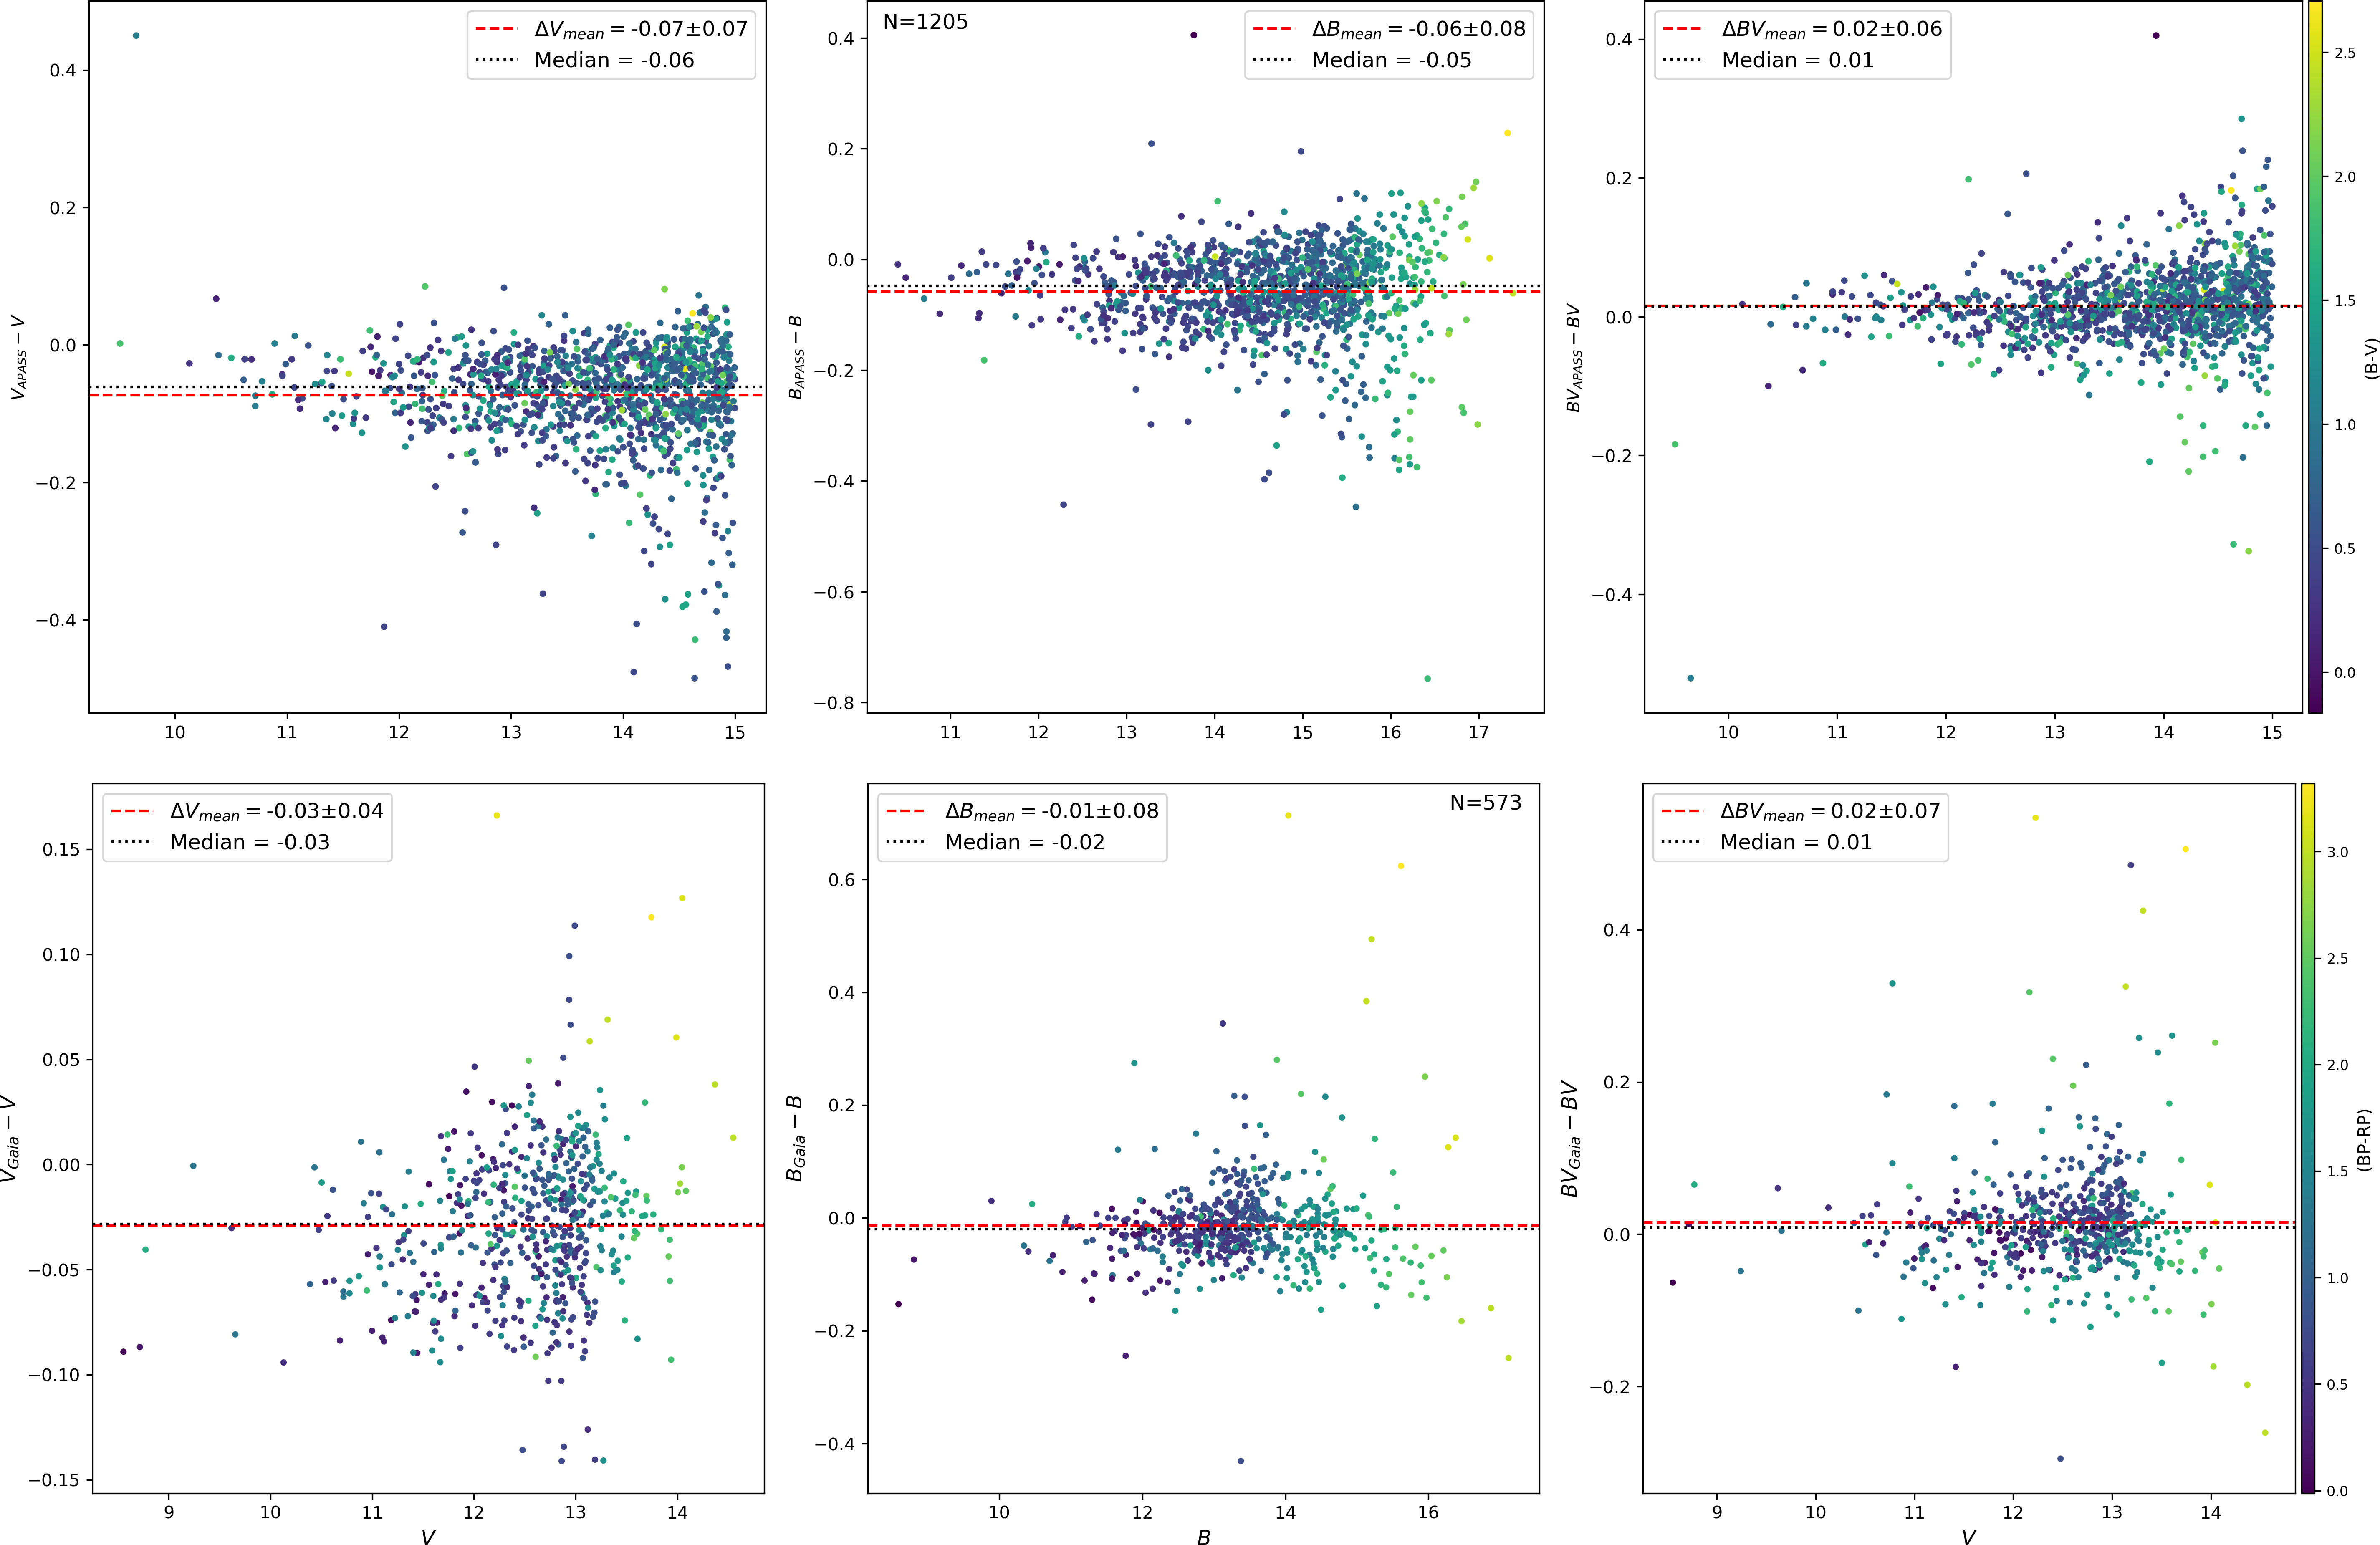
\includegraphics[width=\hsize]{../figs/apass_gaia_V_B_BV.png}   
\caption{Top row: Differences between the APASS DR10 data for the $V$
(left), $B$ (center) magnitudes and $(B-V)$ color (right) and our own
photometry. Bottom row: Same for Gaia DR2 data vs. our photometry. Details
in the text.}
    \label{fig:gaia_transf}
\end{figure*}

Figure \ref{fig:Vim} shows the CCD $V$ images of the clusters areas in which we
carried out the photometric surveys. The series of panels shown from upper
left to the lower right is ordered by increasing longitude and labeled
with the cluster name inserted in every panel. Equatorial decimal
coordinates, $\alpha$ and $\delta$, for the J2000.0 equinox are shown in each
panel as reference.\\

Final tables containing star number, x,y detector coordinates, and $\alpha$,
$\delta$ equatorial coordinates together with magnitude and colors are
accessible in a separate form for each cluster at Vizier.

\begin{figure*}[htp]
    \centering
     \includegraphics[width=1\hsize]{../figs/frames_0.png}   
\caption{V images (charts) of the observed clusters (names inserted)
ordered from top to bottom and from left to right by increasing 
longitude. Decimal $\alpha$ and $\delta$ coordinates for the 2000 equinox are
indicated. North and east are also shown.}
    \label{fig:Vim}
\end{figure*}

\begin{figure*}[htp]
    % \ContinuedFloat
    \addtocounter{figure}{-1}
    \centering
    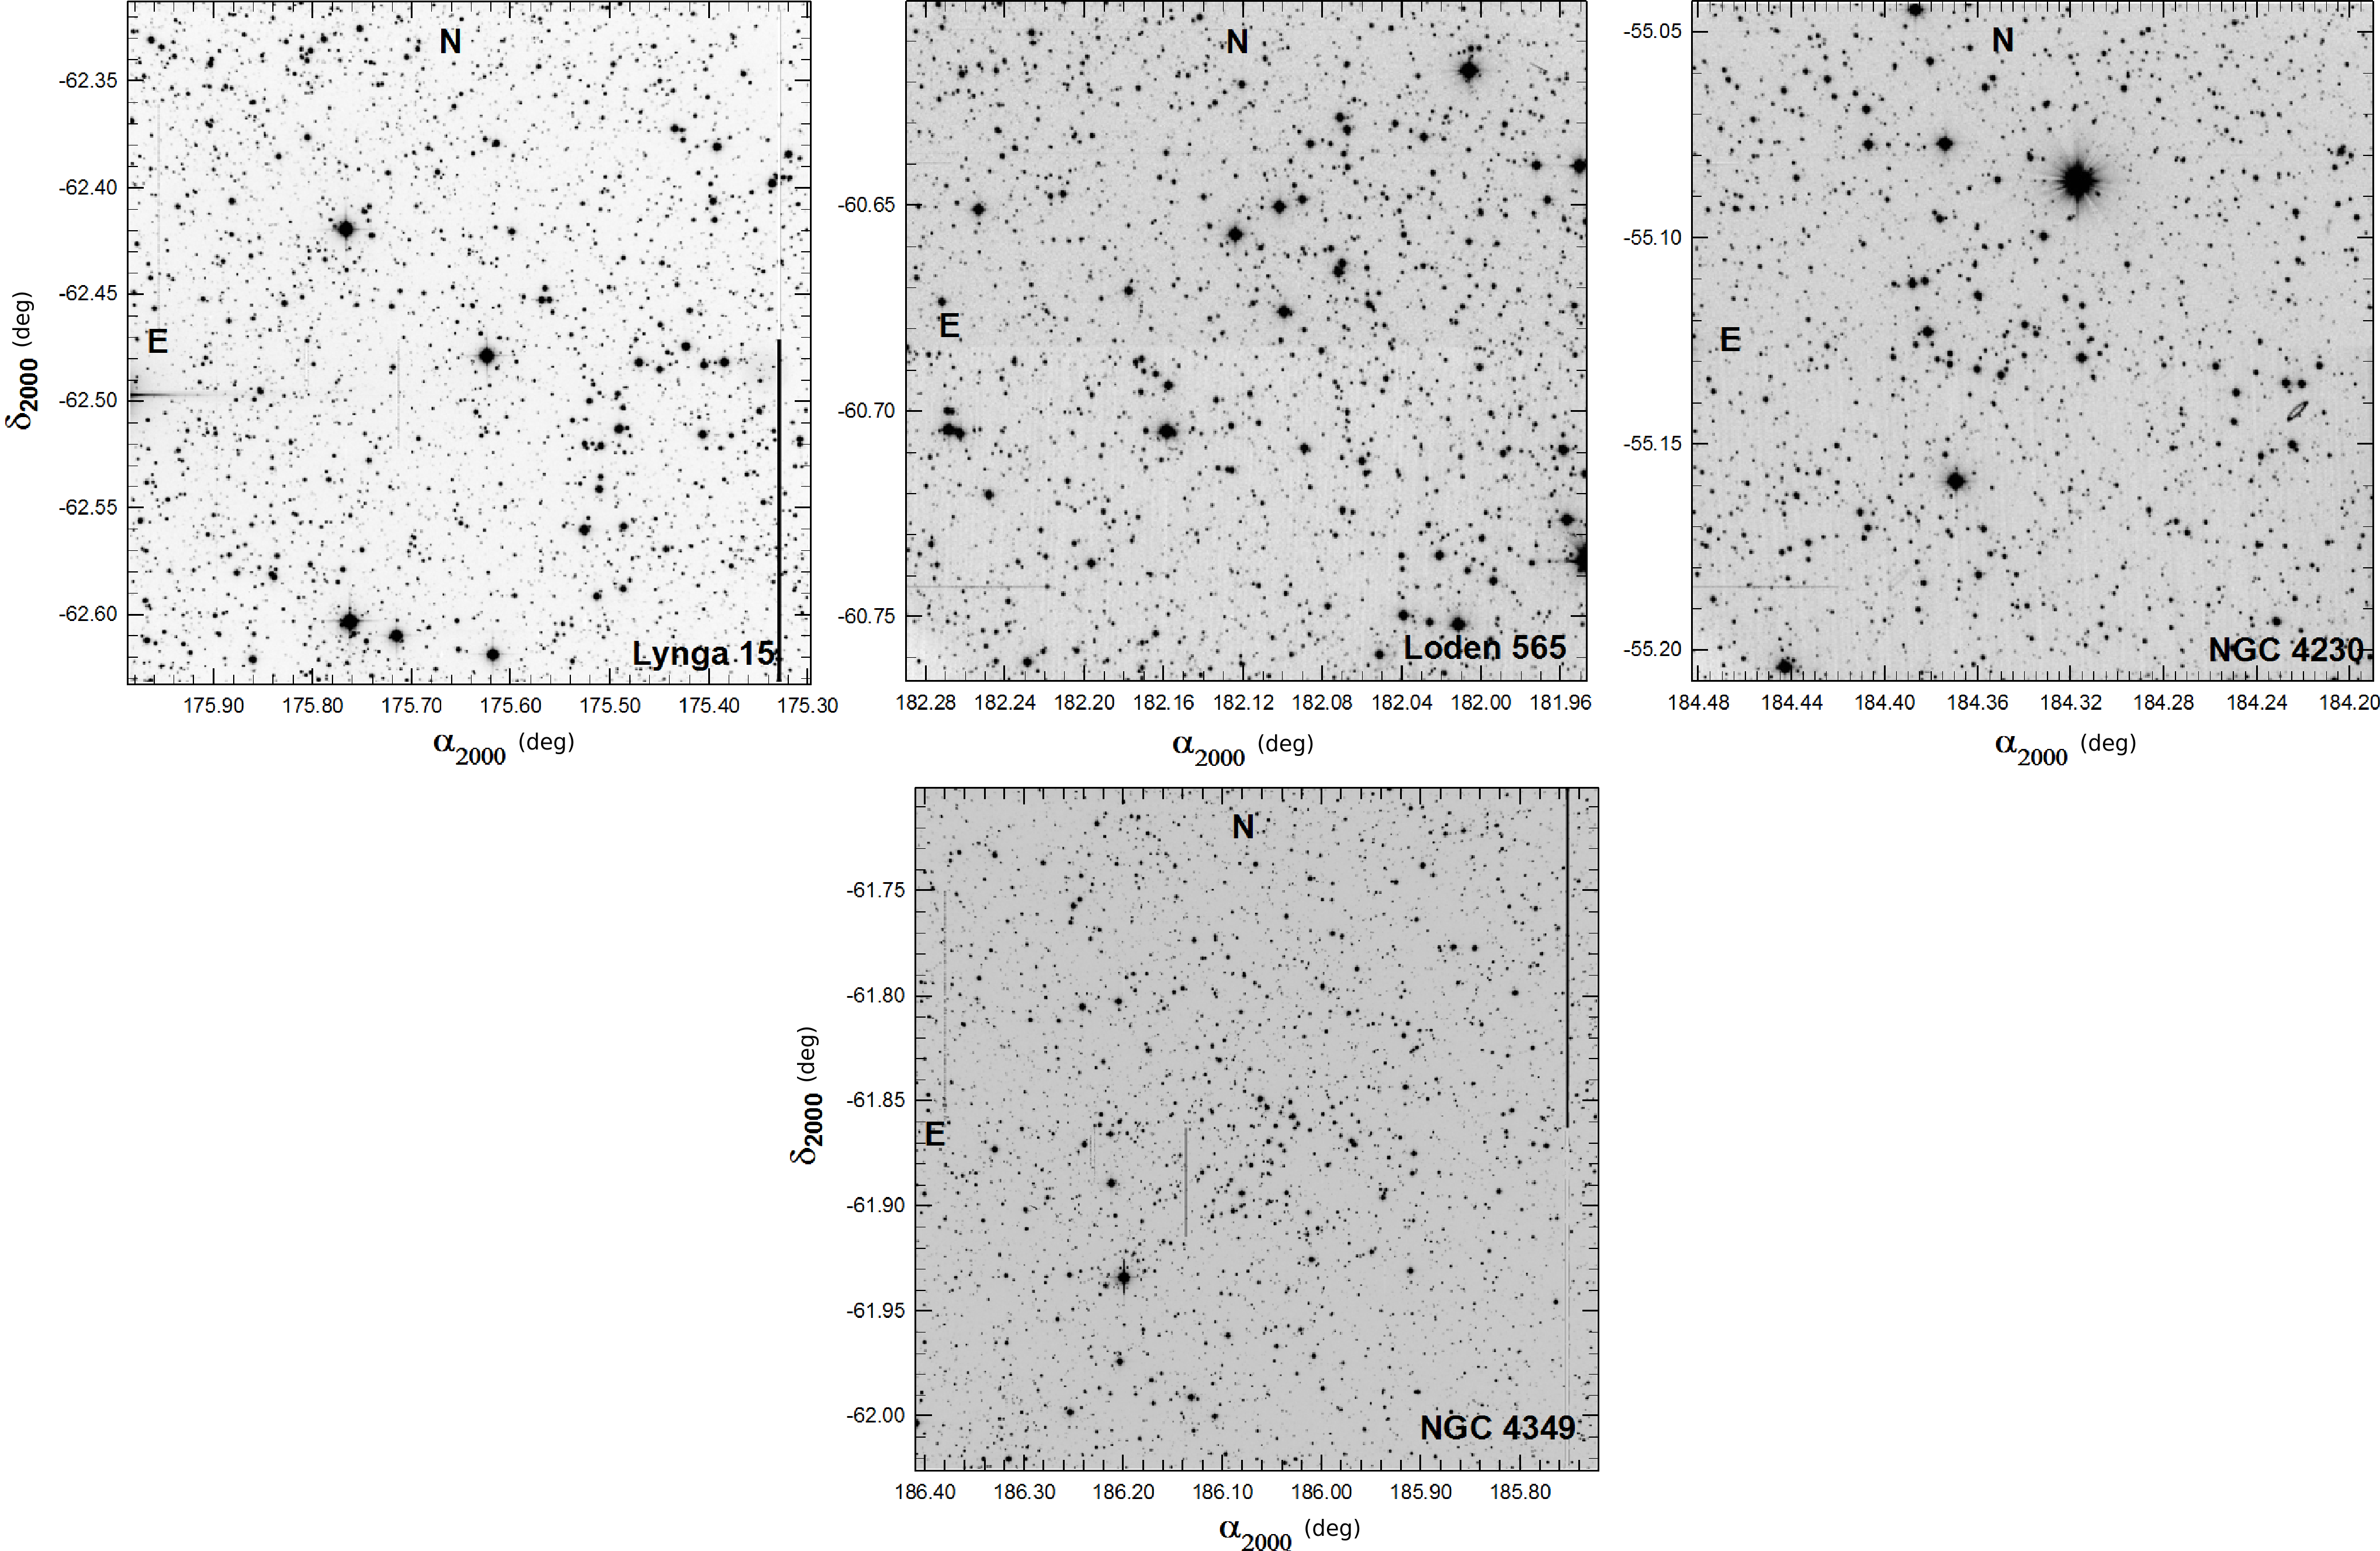
\includegraphics[width=1\hsize]{../figs/frames_1.png}
    \caption{Continued}
    \label{fig:Vim2}
\end{figure*}





%================================================================
\section{Photometric data analysis process: Gaia data and the \texttt{ASteCA}
code}
\label{sec:photom_analysis}

To analyze the large number of objects in a systematic, reproducible, and
homogeneous way, we used the \texttt{ASteCA}
code\footnote{\url{http://asteca.github.io/}}. The main goal of this code is to
put the user apart as far as possible from the analysis of a stellar cluster
to derive its fundamental parameters. We limit ourselves to a brief
summary about the way the positional and photometric data are employed by the
code. A complete description of the analysis carried out by
\texttt{ASteCA} can be found in \cite{Perren_2015} and \cite{Perren_2017}.
%
The basic hypothesis of any stellar cluster analysis is that the
region occupied by a real cluster and the surrounding field show a
priori different properties.
This means that we expect to see an increase in the stellar density  (not always true) where
a cluster is assumed to exist; the kinematic properties of cluster members
are expected to differ from similar ones for the surrounding region; members of a
cluster must be at a same distance, but nonmembers may show any
distance; and the photometric diagrams composed of members of a cluster are expected to
follow a well-defined stellar sequence, but field stars do not. 



% ---------------------------------------------------------------------
\subsection{Gaia data}
\label{ssec:gaia_data}

The second data release for the Gaia mission \citep{GaiaDR2_2018} was presented
in April 2018 with improved coverage, particularly for the five-parameter
astrometric solution.
We crossed-match our complete set of photometric data with those of Gaia DR2
and employed the Gaia $G$ magnitude, parallax, and proper motions in our
analysis as described in Sect~\ref{ssec:asteca_works}.

No uncertainty-based cutoff was imposed on Gaia DR2 parallax or proper
motion data following the advice given in \cite{Luri_2018}, who explained that even parallaxes with negative values or large
uncertainties carry important information. Negative values in the parallax
data were thus retained during the processing. The parallax values
were processed with a Bayesian approach to obtain an independent estimate of the
distance to each cluster. In this approach, the model for the cluster is
taken from the accompanying tutorial by Bailer-Jones on inferring the distance
to a cluster based on astrometry
data\footnote{
\url{https://github.com/agabrown/astrometry-inference-tutorials}}.
The full model (i.e., the likelihood in the Bayesian approach) can be
written as

\begin{equation}
\begin{aligned}
P\left(\{\varpi\} | r_{c}\right)
= & {} \prod_{i=1}^{N} \int \int \frac{1}{2 \pi \sigma_{\varpi_{i}} s_{c}} \\
& \exp \left[-\frac{1}{2} \left( \frac{\left(\varpi_{i}-1 / r_{i}\right)^{2}}{
\sigma_{\varpi}^{2}} + \frac{\left(r_{i}-r_{c}\right)^{2}}{s_{c}^
{2}}\right)\right]
d r_{i}\,d s_{c}
\label{eq:plx_lkl}
\end{aligned}
,\end{equation}

\noindent where $\{\varpi\}$ is the set of all parallax values (our
data), $N$ is the number of processed stars in the cluster,
$\varpi_{i}$ and $\sigma_{\varpi_{i}}$ are the parallax value and its
uncertainty for star $i$, $r_{i}$ is the distance to that star in parsec,
$s_{c}$ is a shape parameter that describes the size of the cluster, and
$r_{c}$ is the distance to the cluster (the parameter we wish to estimate).
%
Our model marginalizes not only over the individual distances ($r_i$;
as done in the original model by Bailer-Jones), but also
over the shape parameter ($s_c$), estimating only the overall cluster distance
$r_c$ using the parallax value and its uncertainty for each star in the
decontaminated cluster region (the membership probabilities process is
described with more detail in Sect.~\ref{ssec:asteca_works}).
%
The prior for the distance in the Bayesian model is a Gaussian centered at a
maximum likelihood estimate of the distance to the cluster region, with a large
standard deviation (1 kpc). This maximum likelihood was
obtained through a differential evolution algorithm built into
\texttt{scipy}\footnote{\url{https://docs.scipy.org/doc/scipy/reference/generated/scipy.optimize.differential_evolution.html}},
applied in Eq. \ref{eq:plx_lkl}, that is, the model.
%
The results of this analysis are shown in Sect~\ref{sec:cluster_discuss}
and are discussed in Sect.~\ref{sec:gaia_distances}.

We include in our analysis a two-sample Anderson-Darling
test,\footnote{\url{https://docs.scipy.org/doc/scipy/reference/generated/scipy.stats.anderson_ksamp.html}}
comparing the distribution of Gaia parallax and proper motions,
between the cluster and the estimated stellar field regions, to quantify how
similar these two regions are.
The results of the test in each case are indicated with AD and the
corresponding p-value\footnote{The null hypothesis ($H_{0}$) is the
hypothesis that the distributions of the two samples are drawn from the same
population. The significance level ($\alpha$) is the probability of mistakenly
rejecting the null hypothesis when it is true, also known as Type I error. The
p-value indicates the $\alpha$ with which we can reject $H_{0}$. The usual 5\%
significance level corresponds to an AD test value of 1.961 for the case of two
samples.} in Fig. \ref{fig:plx_bys_vdBH85} and the similar figures for
the remaining clusters.
The p-value indicates the significance level at which the null hypothesis
can be rejected: the lower the p-value, the higher the probability
for the cluster region to be a true physical entity rather than a random
clustering of field stars. When parallax and proper motions are used, three
p-values are generated that are combined into a single p-value using Fisher's
combined probability
test\footnote{\url{https://docs.scipy.org/doc/scipy/reference/generated/scipy.stats.combine_pvalues.html}}.




% ---------------------------------------------------------------------
\subsection{The way \texttt{ASteCA} works}
\label{ssec:asteca_works}

Since the first release of \texttt{ASteCA,} the code has grown
considerably. The purpose of the tool and the core set of the analysis it is able
to perform are still properly described in \cite{Perren_2015}, although
several modifications have been implemented since. The most relevant changes
include the ability to combine parallax and proper motion data in the
membership analysis algorithm, which was initially purely photometric. This
means that currently, up to seven dimensions of data can be used in this process:
magnitude, three colors, parallax, and proper motions.

The several tasks performed by \texttt{ASteCA} can be roughly divided into three
main independent analysis blocks: structural study including the
determination of a cluster region identified primarily by an overdensity,
individual membership probability estimation for stars inside the overdensity,
and the search for the best-fit parameters.\\

The first block estimates center and radius values that in each case define the
cluster region. Reliable estimates of these two quantities can only be achieved
when a clear overdensity and a large number of members are detected.
If a cluster is not clearly defined as an overdensity in the observed frame and
if its boundaries are weakly established, \texttt{ASteCA} allows center and
radius to be manually fixed because the automatic procedure may return incorrect
values. We chose to fix all radius values manually because many of
our observed frames are structurally sparse and with a low number of members,
and display very noisy radial density profiles (hereafter RDP).\footnote{
The radius values are estimated using the frames in pixel coordinates,
and then converted into arcminutes.
}
%
Every point of the RDP was obtained by generating rings around the
center defined for the potential cluster, that is, the comparison field.
%
In our case, the comparison field may contain between one and ten regions
with an area equal to that of the cluster, depending on the cluster area and the
available size of the remaining frame. In each ring the number of
stars (with no magnitude cut applied) is divided by the respective
area to obtain a value of the radial density.
%
To compute the density level of the field (foreground and background),
outliers in the RDP are iteratively discarded to avoid biasing the final value.
This procedure is repeated until it converges to an equilibrium value, equivalent
to the density of the stellar field at a given distance from the potential
cluster center.

King profile \citep{King_1962} fittings were performed when
a fit could be generated. No formal core or tidal radius are given because
their values, due mainly to the shape of the RDP, were not within reasonable
estimates (the process to fit the King profiles to the RDP returned either
high and unrealistic values, or values with very large uncertainties).
This might be due to the nonspheric geometry of sparse open clusters
combined with the field contamination within the cluster region. Although
photometric incompleteness is not taken into account in the generation of the
RDP, these clusters are not strongly affected by crowding; thus we do not
expect this to have a major effect on the estimated radii.\\

The second block assigns membership probabilities to the defined
cluster region, an often disregarded process in simpler cluster studies, 
and \textbf{removes the most probable field stars that contaminate this region}.
By itself, an overdensity does not guarantee the presence of a real cluster;
 an overdensity is frequently generated by random fluctuations in the field stellar
density. To avoid this mistake, the properties for cluster and
field stars must be compared. Ideally, we search for firm evidence of
a cluster sequence at some evolutionary stage. \texttt{ASteCA} employs a
Bayesian algorithm to compare the photometric, parallax, and proper motion
distribution of the stars in the cluster region with a similar distribution in
the surrounding field areas \citep{Perren_2015}. Initially, the analysis
was carried out in an N-dimensional data space that combined the
$G$ magnitude, parallax, and proper motions from Gaia with colors from our own
photometry: $(V-I)$, $(B-V)$, $(U-B)$. In this case, the data space where
the algorithm works is therefore characterized by N=7.
Combining all the available data is not always optimal, however. A
data dimension can sometimes introduce noise in the analysis instead of helping
distinguish members from field stars. In our case, we found that using
parallax and proper motions, that is, N=3, resulted in more clearly defined
cluster sequences than when we included photometric dimensions (with N=7 as
mentioned above).

%
Briefly, the algorithm compares the properties of this N-dimensional data space
for stars inside (cluster region) and outside (field region)
the adopted cluster limits. All the data dimensions are previously normalized 
(to prevent any dimension from outweighting others) and 4 $\sigma$ outliers are
rejected.
The position of every star inside the cluster in this data space is compared
against each star in all the defined equivalent-area field regions,
assuming a Gaussian probability density (centered at the given values for each
data dimension, with standard deviations given by the respective
uncertainties). This procedure is repeated hundreds or thousands of times 
(defined by the user), each time selecting different stars to construct an
approximation of the clean cluster region. The result of this
algorithm is thousands of probability values that are averaged to a final
single membership probability value for each star within the cluster region.

This block ends with the cleaning of the photometric diagrams in the cluster
region. The photometric diagram of each cluster region is divided into cells, and
the same is done for the equivalent diagram of the field regions. The stellar
density number found in the field is then subtracted from the cluster
photometric diagram, cell by cell, starting with stars that have low
membership probabilities. Therefore, the final cluster photometric diagrams
contain not only star membership assignations, but are also cleaned from the
expected field stellar contamination. This two-step process is of the utmost
importance to ensure that the fundamental parameter analysis that
follows is performed on the best possible approximation to the cluster
sequence (particularly when the cluster contains only few members).\\

Finally, the third block estimates the cluster parameters by minimizing a
likelihood function \citep{Dolphin_2002} through employing a numerical
optimization with a genetic algorithm \citep{Charbonneau_1995}. This last
stage includes the assignment of uncertainties for each fitted parameter with a
standard bootstrap method \citep{efron1986}. Again, all of these processes are
described in much more detail in \cite{Perren_2015} and \cite{Perren_2017}.

It is worth noting that unlike other tools \citep[e.g.,][]{Yen_2018},
\texttt{ASteCA} does not fit isochrones to cluster sequences in photometric
diagrams. Instead, it fits synthetic clusters generated from a set of
theoretical isochrones, a given initial mass function, and completeness and
uncertainties functions estimated directly from the observations.
These synthetic clusters are represented as two- or three-dimensional
CMDs, depending on the number of photometric colors
available in our observations. The best-fit isochrones shown in green in
the photometric diagrams in Fig.~\ref{fig:fundpars_vdBH85} for vdBH85 (and
similar figures for the remaining clusters) are there for convenience
purposes only, as a way to guide the eye.

The code makes use of the PARSEC v1.2S \citep{Bressan_2012} theoretical
isochrones (obtained from the CMD
service\footnote{\url{http://stev.oapd.inaf.it/cgi-bin/cmd}}), and the
\cite{Kroupa_2002} form for the initial mass function. A dense grid of
isochrones with fixed $z$ and $\log(age)$ values is requested to the CMD
service\footnote{Grid values: $z$ range [0.0005, 0.0295] with a step of
0.0005; $\log(age)$ range [7, 9.985] with a step of 0.015}, which are later
used in the fundamental parameters estimation
process. The full processing yields five parameters: metallicity, age,
extinction, distance, and mass, along with their respective uncertainties. The
binary fraction was always fixed to 0.3, a reasonable
estimate for open clusters \citep{Sollima_2010}. As for the final mass of each
cluster, although the values are corrected by the effects of star loss
due to photometric incompleteness at large magnitudes and the
percentage of rejected stars with large photometric uncertainties, it is not
corrected by the dynamical mass loss due to the cluster's orbiting through the
Galaxy. Hence, it should be regarded as a lower limit on the actual initial
mass value.

From a practical point of view, the code proceeds as follows to estimate the
cluster parameters: First, individual three-dimensional $G$ vs $(B-V)$ vs $
(U-B)$ photometric diagrams are analyzed, for which the metallicity is fixed to
a solar value ($z = 0.0152$) in order to reduce the dimensionality of the
parameter space, and thus its complexity. Although several of the diagrams
described above in our case contain a rather small number of stars because of
the $U$ filter, they are very useful to obtain reddening and thus
extinction by inspecting the $(U-B)$ vs $(B-V)$ diagrams
\citep[e.g.,][]{Vazquez2008} .
%
The individual $E(B-V)$ values in each region were always verified against
the maximum values given in the \cite{Schlafly_2011} maps (hereafter
S\&F2011)\footnote{Through the
NASA/IPAC service \url{https://irsa.ipac.caltech.edu/applications/DUST/}}.
The only information extracted from this first step, and in particular,
by inspecting the $(U-B)$ vs $(B-V)$ diagram, is thus a reasonable range for
the $E(B-V)$ parameter.
%
Second, the analysis of the $G$ versus $(B-V)$ versus $(V-I)$ diagram is carried out
by restricting now the reddening space to the $E(B-V)$ range obtained previously,
while still fixing the metallicity to solar value. From this process we obtain
estimates for the age, distance, and cluster mass.
%
Finally, in a third stage, the parameter ranges derived above are applied, now
including the metallicity as a free parameter.
As a result of the entire procedure, we obtain a five-parameter best-fit model
for each observed cluster, along with the associated one $\sigma$ uncertainties
for each one. In all the cases we adopted $R=A_v/E(B-V) = 3.1$ to produce 
absorption-free distance moduli.

During the maximum likelihood and bootstrap processes,
each observed cluster was compared to $\sim2\times10^7$
synthetic clusters. This number was obtained by combining the synthetic
clusters that were generated in the maximum likelihood and bootstrap processes by
varying the fundamental parameter values.




%================================================================
\section{Cluster-by-cluster discussion of the structural and intrinsic
parameters provided by \texttt{ASteCA}}
\label{sec:cluster_discuss}

We now present the results from the spatial and photometric analysis
carried out with \texttt{ASteCA}, together with the outcome of the application
of the Anderson-Darling test that compares parallax and proper motion
distributions in cluster regions with their respective field regions.
It is important to emphasize that the code always fits the
best possible synthetic cluster to a given stellar distribution, regardless of 
whether it is a true open cluster or not.

Our sample contains clusters with a wide variety of properties: some are
bright, clearly detached from the cluster background and therefore have a
clearly defined main sequence (TR 13, TR 12, NGC 4349, vdBH 87, and vdBH 92).
Others are faint, with a sparse star population and are easy to
confuse with the background (vdBH 73, vdBH 85, vdBH 106, RUP 162, and RUP 85).
Because we include very many figures in this paper, we therefore decided to
add these sources to an appendix. We limit ourselves here to presenting
the case of three extreme types of clusters according to the statement
above: a poorly defined (vdBH 85) and a well-defined cluster (NGC 4349), and a
source that is not a cluster (RUP 87).






% ---------------------------------------------------------------------
\subsection{van den Bergh-Hagen 85}
\label{ssec:vdbh85}

\begin{figure*}[ht]
    \centering
    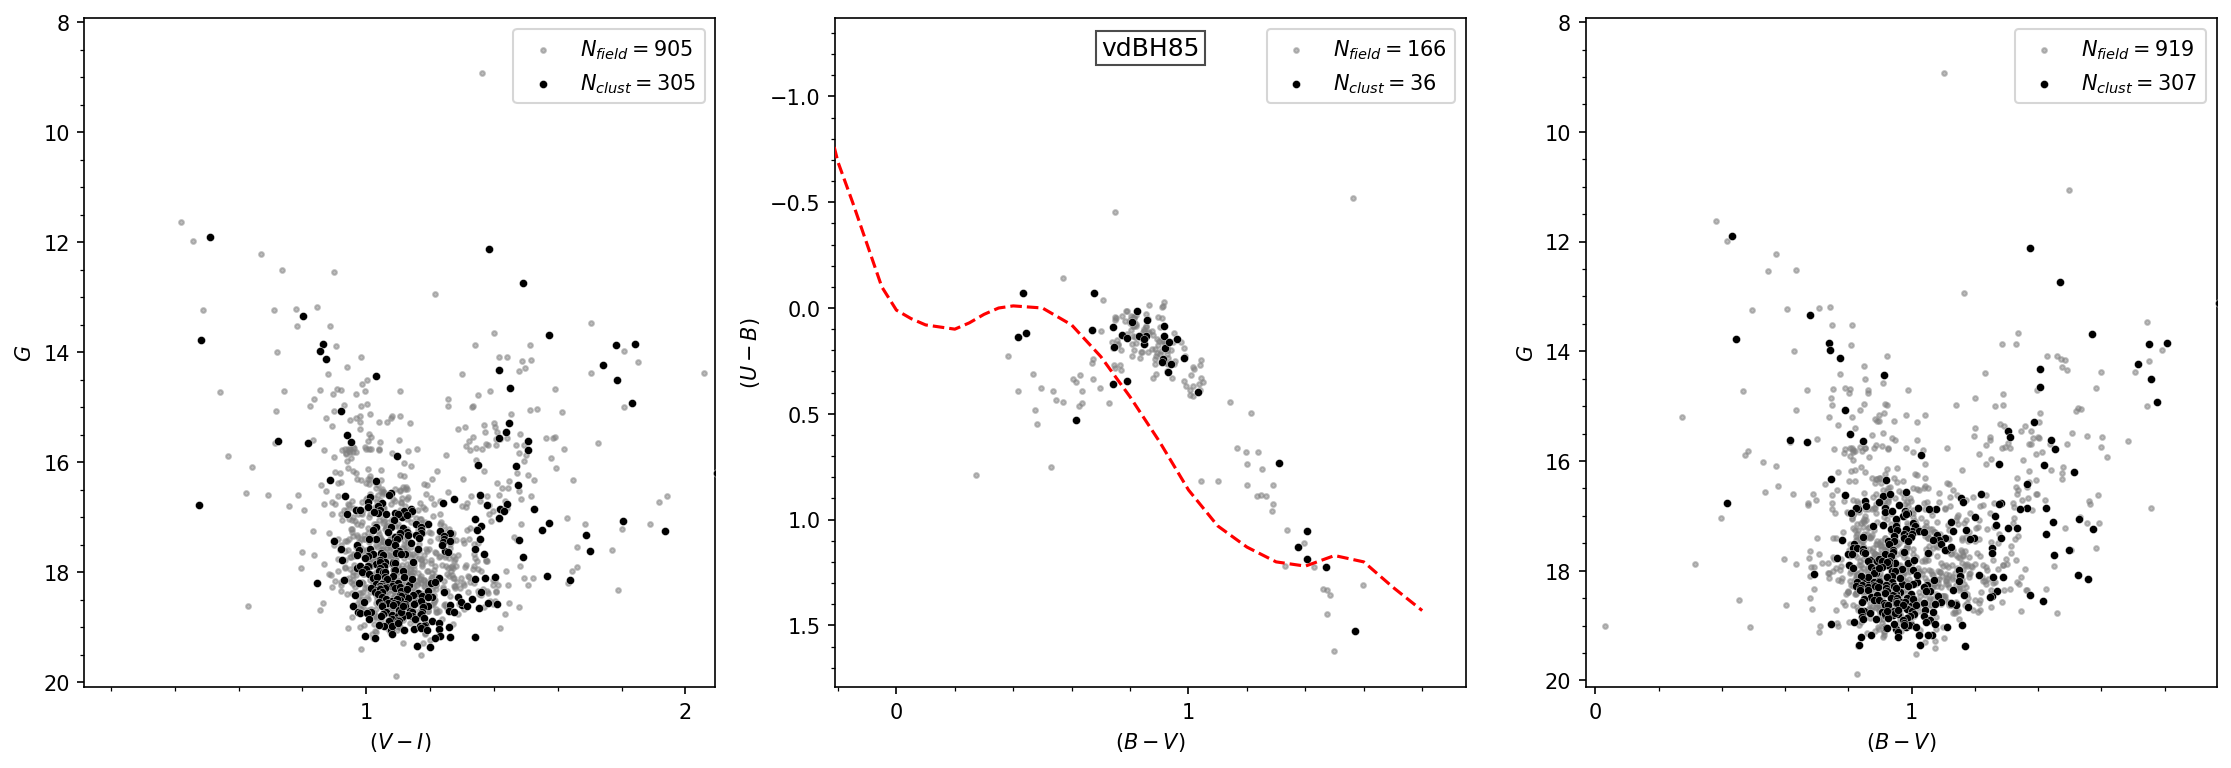
\includegraphics[width=\hsize]{../figs/obs_vdBH85.png}
\caption{From left to right: $G$ vs. $(V-I)$, $(B-V)$ vs. $(U-B)$, and
$V$ vs. $(B-V)$ diagrams for all the stars observed in the region of van
den Bergh-Hagen 85.
The red dashed line in the CCD shows the position of the ZAMS
\citep{Aller1982}. Insets in each diagram contain the number of stars 
in the cluster region ($N_{clust}$, black circles) and in the surrounding
field ($N_{field}$, gray circles).
}
    \label{fig:photom_vdBH85} % fig11
\end{figure*}

\begin{figure*}[ht]
    \centering
    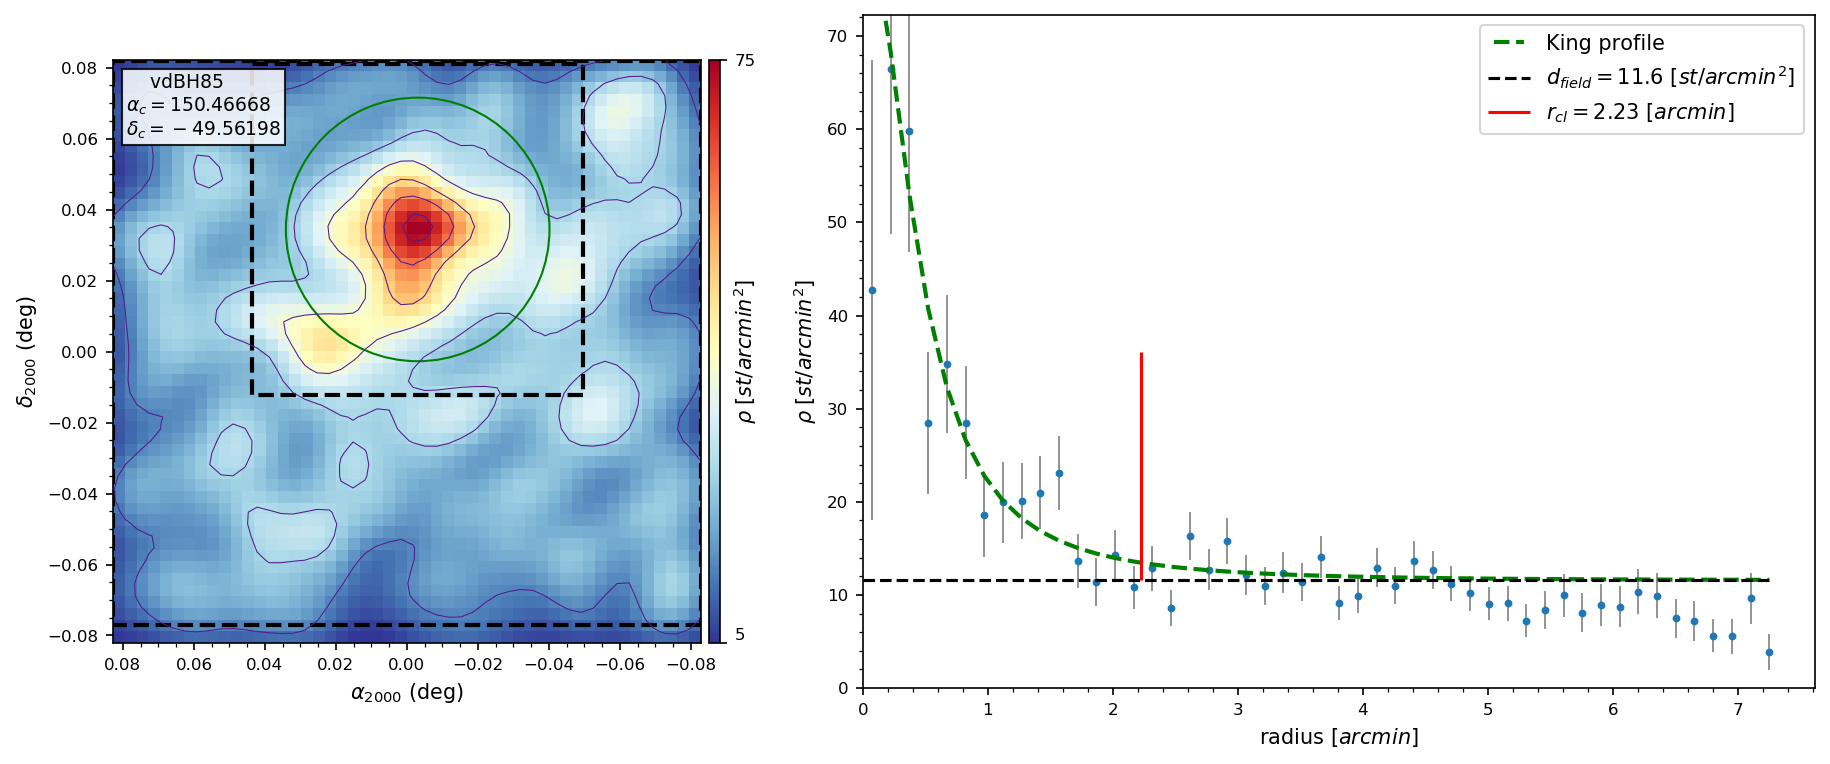
\includegraphics[width=\hsize]{../figs/dmap_vdbh85.png}
\caption{From left to right, we present in the first panel
a contour plot showing the position of the overdensity associated with vdBH 85.
The green inner circle shows the cluster size, and the two black dashed-line
squares enclose the region that \texttt{ASteCA} used to estimate the field
stellar properties. The lower density values at the frame borders are an
artifact of the kernel density estimate method that we employed to generate the density
maps.
Equatorial coordinates in decimal format are indicated.
The color bar denotes the star number per square arcminute (linear scale).
These values are slightly different from those in the panel to the right
because they are obtained with a different method (nearest neighbors).
%
The second panel shows the RDP as blue dots with standard deviations as
vertical black lines. The King profile is shown as a dashed green line. The
horizontal black line is the mean field stellar density. The vertical red line is the
adopted cluster radius.
}
    \label{fig:struct_vdBH85}
\end{figure*}

\begin{figure*}[ht]
    \centering
    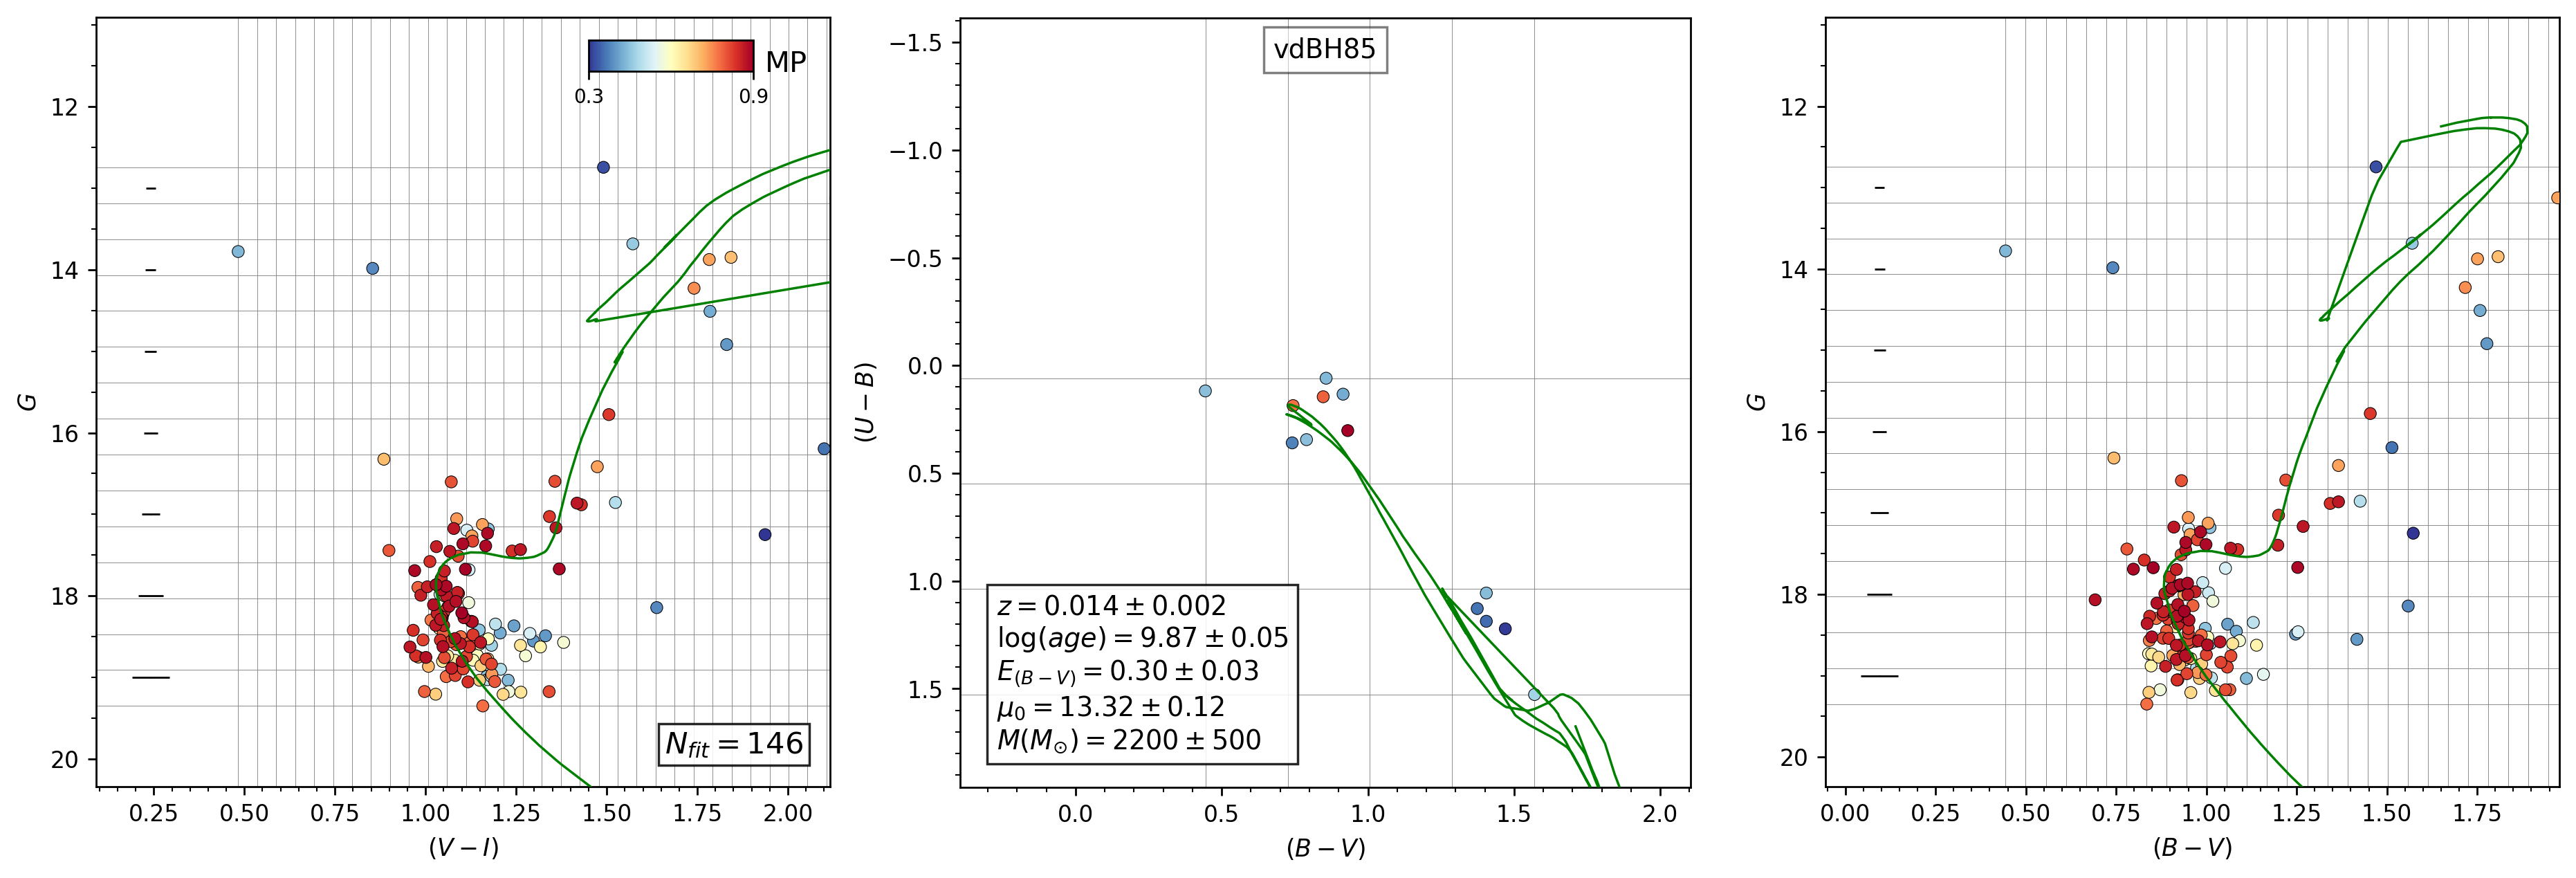
\includegraphics[width=\hsize]{../figs/cmds_vdBH85.png}
\caption{From left to right: $G$ vs. $(V-I)$ , $(B-V)$ vs. $(U-B)$,
and $G$ vs. $(B-V)$ clean diagrams after field interlopers
were removed by \texttt{ASteCA} over vdBH 85. The color of each star reflects
its membership probability \textbf{(MP)}. Corresponding values are in the color bar at
the upper right corner in the $G$ vs. $(V-I)$ diagram (left) labeled
MP. The CCD in the middle always shows fewer stars because of the $U$ filter.
The grid lines trace the edges of the three-dimensional photometric histograms we used
to evaluate the likelihood function described in Sect~\ref{ssec:asteca_works}.
The inset in the lower right corner in the $G$ vs. $(V-I)$ diagram shows
the number of stars used by \texttt{ASteCA} to compare with synthetic clusters.
The inset in the middle panel includes the final
results for metallicity, $\log(age)$, $E(B-V)$, the corrected distance
modulus, and the total cluster mass provided by \texttt{ASteCA}. The green
continuous line in the three diagrams is a reference isochrone. In
particular, the green line in the CCD, middle panel, shows the
most probable $E(B-V)$ value fitting found by \texttt{ASteCA}.
}
    \label{fig:fundpars_vdBH85}
\end{figure*}

\begin{figure*}[ht]
    \centering
    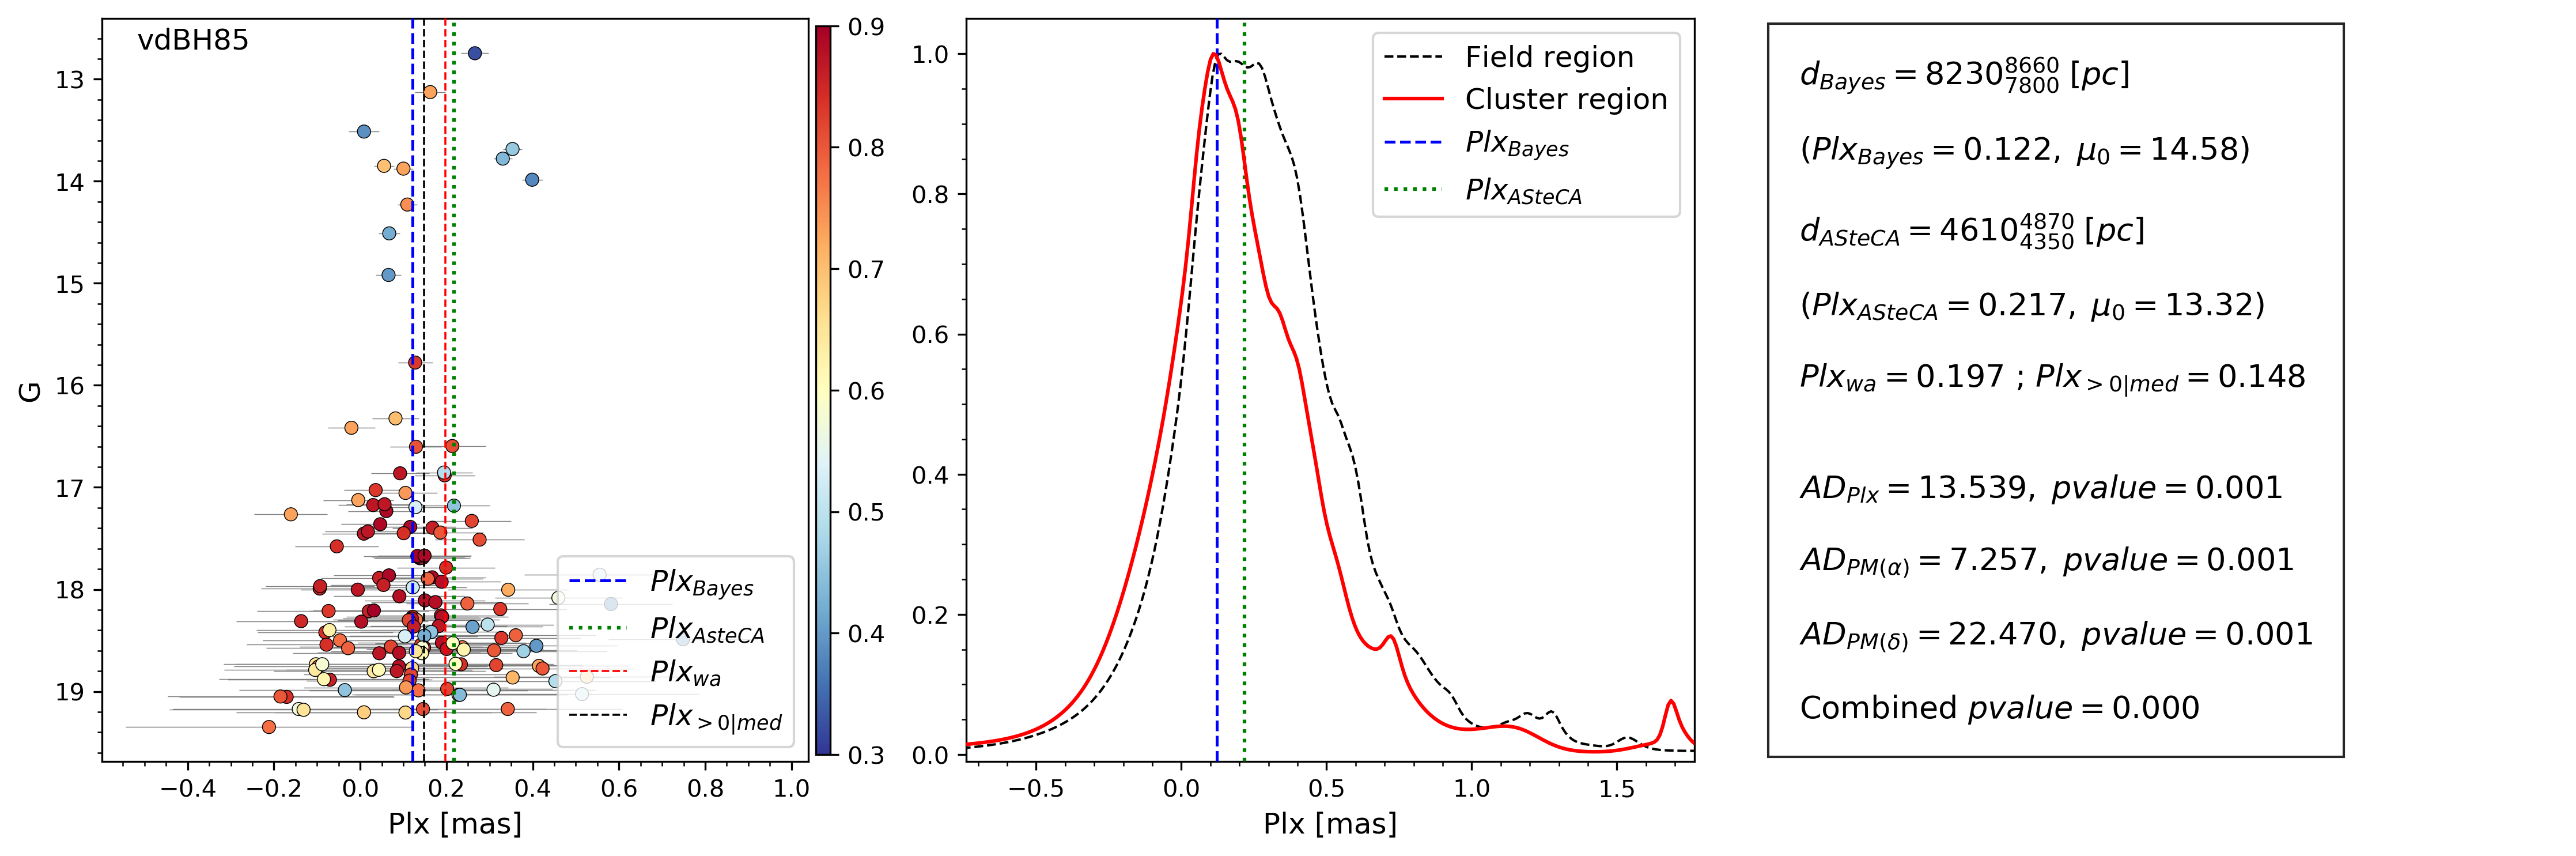
\includegraphics[width=\hsize]{../figs/plx_vdBH85.png}
\caption{Left panel: Distribution of the parallax for all stars with membership
probabilities in the cleaned cluster region as a function of the apparent
magnitude $G$ (the vertical color scale shows the membership
probability of the star) in vdBH 85.
Horizontal bars represent the parallax errors as given by Gaia. The different
parallax value fittings are shown by dashed lines of different colors:
blue shows the Bayesian parallax estimate, green the \texttt{ASteCA}
photometric distance, red the weighted average, and black the median 
(without negative values).
The middle panel is a normalized comparison between the parallax
distributions inside (red line) and outside the cluster region (dashed
black line). The frame at the right summarizes the distances in parsecs
according to the Bayesian analysis ($d_{Bayes}$) and \texttt{ASteCA} ($d_
{ASteCA}$), followed by the corresponding parallax value, $Plx$, and
corrected distance modulus ($\mu_0$). Both fittings are indicated by the
vertical blue and green dashed lines. The last four text lines in the right
panel list the AD values for $Plx$, $PM(\alpha)$, and $PM(\delta),$ followed by
the corresponding $p$-values, and finally, the combined $p$-value.
}
    \label{fig:plx_bys_vdBH85}
\end{figure*}

The open cluster vdBH 85 appears in the sky slightly east of the center of the
Vela constellation. The $V$ chart in Fig. \ref{fig:Vim} shows a weak star
concentration near the north side of the observed field that extends slightly
to the southeast. 
%
The color-color and color-magnitude diagrams (from now on CCD and CMDs,
respectively) of the entire field of view in Fig.~\ref{fig:photom_vdBH85} is
just a dispersed stellar distribution that approximately ends in a compact accumulation at
$(B-V)=1$ and below $G=17$ mag. Another clear feature is the
structure at $G=16$ mag in the two CMDs and for $1.2<(B-V)<1.7$ mag, which resembles
a red clump.\\

Figure \ref{fig:struct_vdBH85} represents the spatial analysis carried
out by \texttt{ASteCA}: results from the search for a stellar
overdensity, the mean value for the stellar field density, the respective King
profile attempting to fit the radial density profile, and the assumed radius.
%
\texttt{ASteCA} detected an overdensity here that is difficult to see in
Fig.~\ref{fig:Vim}. It stands out from the stellar background that is contained
in a radius of 2.2 arcmin. It is characterized by a smooth RDP 
with nearly six times the background density at its peak, 
as shown in Fig.~\ref{fig:struct_vdBH85}.\\

In the following step, the removal of interlopers by comparison with the
background field properties yields the field-decontaminated CCD
$(U-B)$ versus $(B-V)$ and CMDs, $G$ versus $(B-V),$ and $G$ versus $(V-I)$.
This removal was performed by comparing the stellar density in the photometric
diagram of the cluster \textbf{region} (whose stars already have membership
probabilities provided by \texttt{ASteCA}) with that of the surrounding field
regions. These diagrams are shown in Fig.~\ref{fig:fundpars_vdBH85}.
%
We insert the results from the best synthetic cluster fitting to the field
decontaminated diagrams in the middle panel of Fig.~\ref{fig:fundpars_vdBH85}.
In these three panels we also show the isochrone curves from which the best
synthetic cluster fit was generated. These isochrones were generated
using the maximum likelihood values found for the metallicity and age by
averaging of theoretical isochrones taken from the employed grid.
Again, this is just to guide the eye because \texttt{ASteCA} does not fit
isochrones.

After the membership probabilities were established and field
interlopers were removed, the two CMDs of all stars show a short but evident main
sequence below $G=17$ mag.
Three magnitudes above the cluster turn-off, several stars appear at $G=14$ mag. They might be part of the bright end of the giant branch. The comparison
with the best fit of a synthetic cluster shows the following
characteristics for vdBH 85:

\begin{itemize}
\item [a)] The cluster is seen projected against a stellar field with moderate
    to low color excess. The best value corresponds to $E(B-V)=0.3,$ which
    agrees with the maximum value of 0.46 mag stated by S\&F2011.
\item [b)] The free absorption distance modulus of vdBH 85 is
    $13.32\pm0.12$ mag, which implies a distance of $4.61\pm0.26$ kpc
    from the Sun.  This by itself explains the extreme weakness of the
    cluster members.
\end{itemize}

Figure \ref{fig:plx_bys_vdBH85} includes three panels. The
left panel shows the $G$ mag versus Gaia parallax values (uncertainties indicated by
horizontal bars) of cluster members, colored according to the estimated
membership probabilities (color bar to the right).
%
The Bayesian distance ($d_{Bayes}$) found by the code is shown here by
a vertical blue dashed line, the equivalent \texttt{ASteCA} distance
($d_{ASteCA}$) with the green dotted line, the weighted average with the red dashed
line (where the weights are the inverse of the parallax
errors), and the naive estimate of obtaining the median of stars with
parallax values greater than zero with the black dashed line.
%
The middle panel shows the kernel density estimate of stars in the surrounding
field region and the cluster region with black and red lines, respectively. For
the Anderson-Darling test we used all the stars within the cluster region with
Gaia data. In the right panel we summarize the distances in parsecs and errors,
($d_{Bayes}$) and $d_{ASteCA}$, followed by the corresponding parallax
value, $Plx$, and corrected distance modulus, $\mu_0$. Both fittings are
indicated by the vertical blue and green dashed lines. The final
four text lines in the right panel list the AD values for $Plx$, $PM(\alpha)$, and
$PM(\delta)$ from the Anderson-Darling test, followed by the corresponding
$p$-values, and finally, the combined $p$-value.

The distance estimated with parallax data from Gaia is almost 4 kpc
larger than the distance obtained through the photometric analysis. This is most
likely a failure of the Bayesian inference method we employed, and is caused by the large
uncertainties associated with most of the probable cluster members. Further
discussion is presented in Sect. \ref{sec:gaia_distances}.
%
The Anderson-Darling test results in Fig. \ref{fig:plx_bys_vdBH85} suggest that the
null hypothesis can be safely rejected given the combined $p$-value of
0.0. The $Plx$, $PM(\alpha),$ and $PM(\delta)$ results from the
Anderson-Darling test leave no doubt that cluster region and surrounding comparison field come from quite different stellar populations.\\

We conclude that this object is a real and very old cluster, the oldest in our
sample, approximately $7.50\pm0.80\times10^9$ yr old. This age places
vdBH85 among the ten oldest clusters cataloged in the
WEBDA\footnote{\url{https://webda.physics.muni.cz/}} and
DAML\footnote{\url{http://cdsarc.u-strasbg.fr/viz-bin/cat/B/ocl}}
\citep{Dias_2002} databases.




% ---------------------------------------------------------------------
\subsection{NGC 4349}

\begin{figure*}[ht]
    \centering
    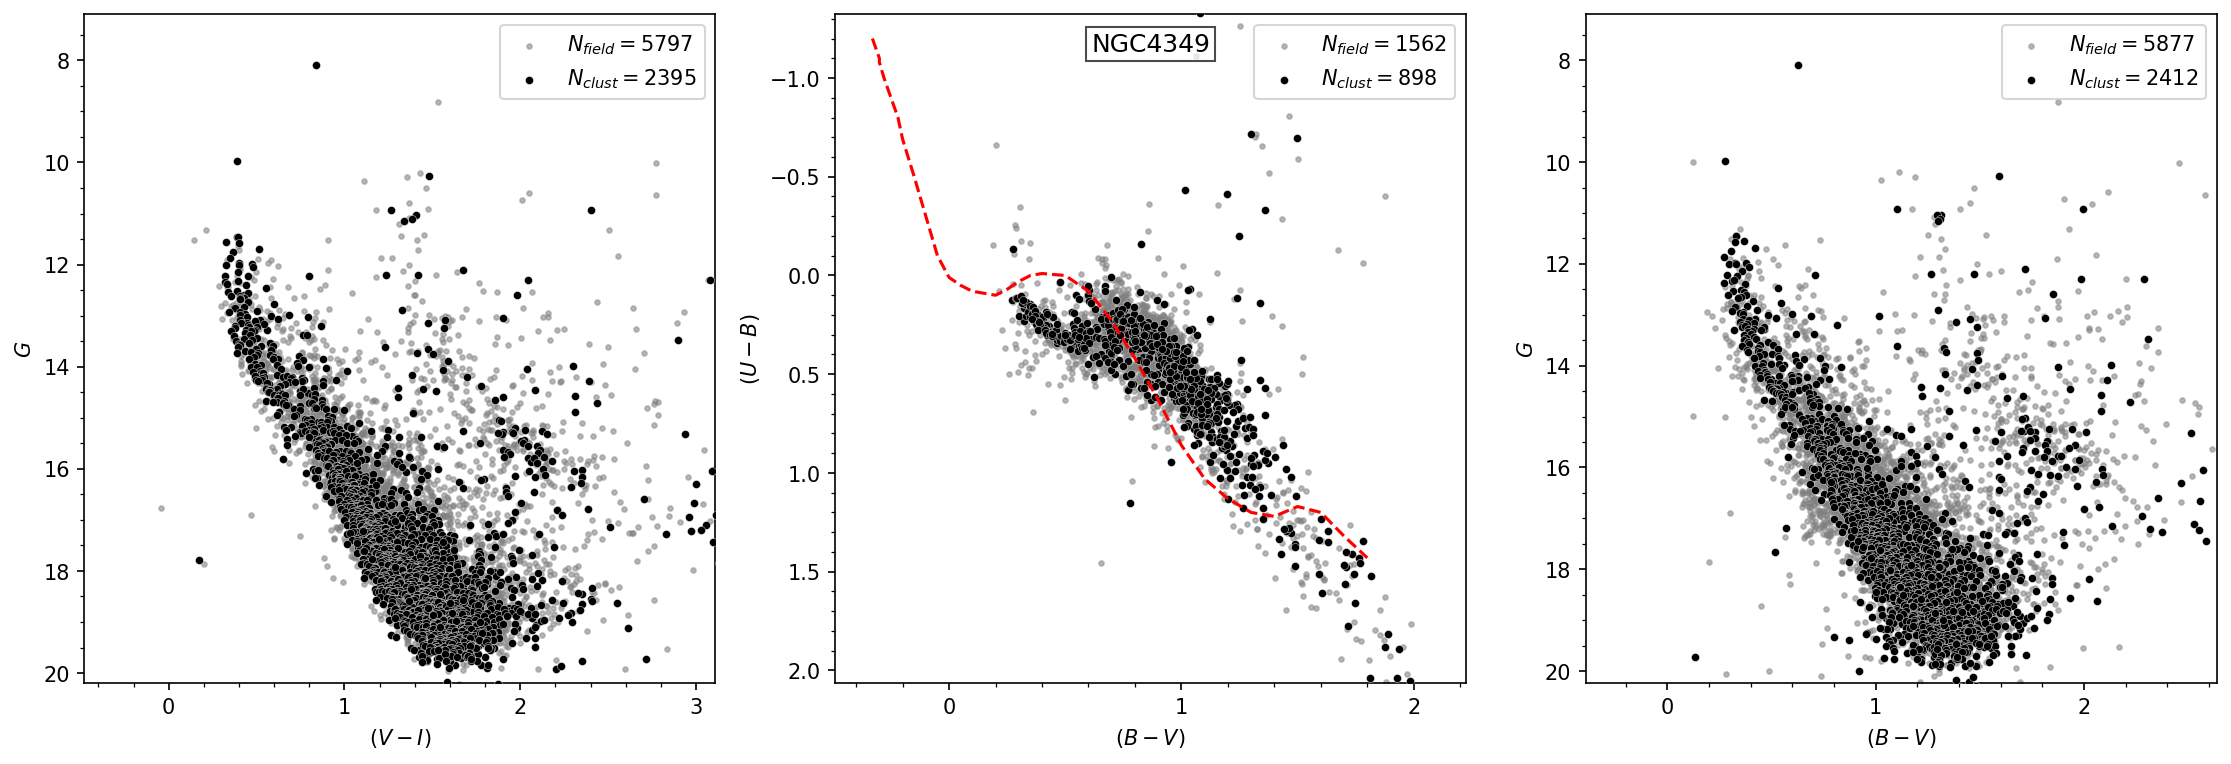
\includegraphics[width=\hsize]{../figs/obs_NGC4349.png}
    \caption{Idem Fig. \ref{fig:photom_vdBH85} for NGC 4349.}
    \label{fig63}
\end{figure*}
\begin{figure*}[ht]
    \centering
    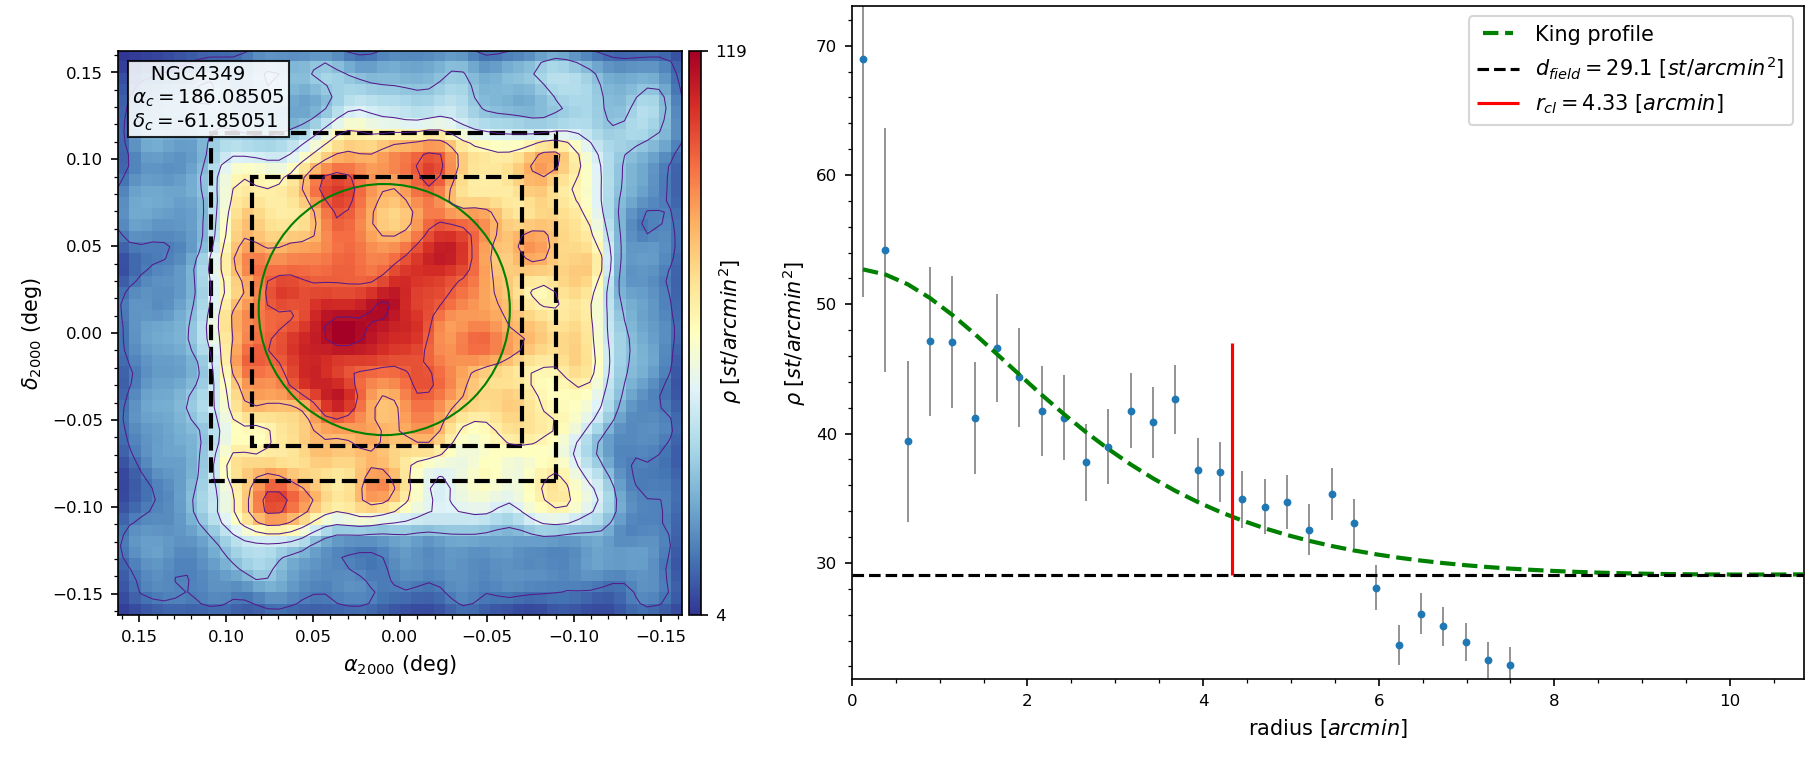
\includegraphics[width=\hsize]{../figs/dmap_ngc4349.png}
    \caption{Idem Fig. \ref{fig:struct_vdBH85} for NGC 4349.}
    \label{fig64}
\end{figure*}
\begin{figure*}[ht]
    \centering
    \includegraphics[width=\hsize]{../figs/cmds_ngc4349.png}
    \caption{Idem Fig. \ref{fig:fundpars_vdBH85} for NGC 4349.}
    \label{fig65}
\end{figure*}
\begin{figure*}[ht]
    \centering
    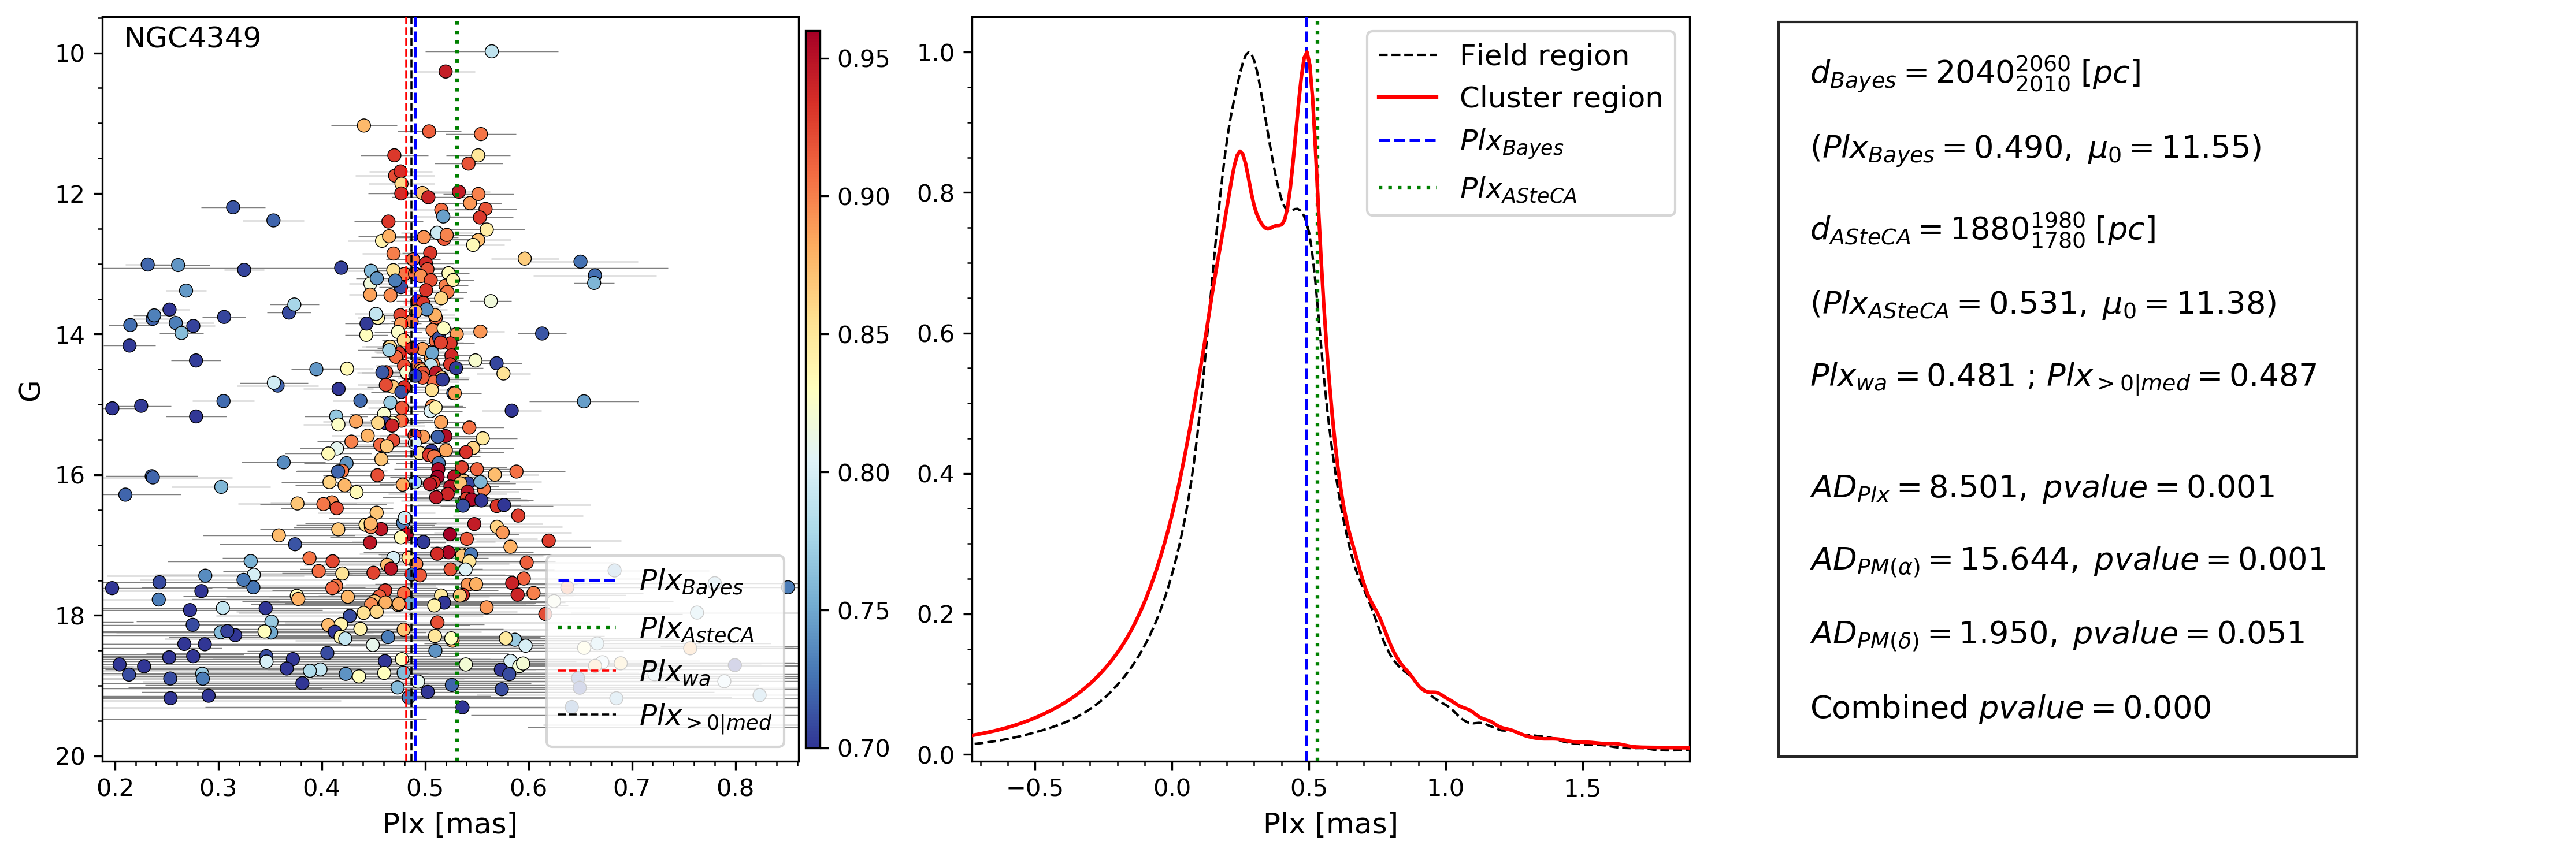
\includegraphics[width=\hsize]{../figs/plx_NGC4349.png}
    \caption{Idem Fig. \ref{fig:plx_bys_vdBH85} for NGC 4349.}
    \label{fig:plx_bys_NGC4349}
\end{figure*}


This is an object in the Crux constellation, placed slightly south of its
geometric center. At first glance, the $V$ image in Fig. \ref{fig:Vim} shows a
distinguishable star accumulation. The overall photometric CCD and CMDs in
Fig.~\ref{fig63} show a prominent stellar sequence emerging at $G\approx15$ mag
from the usual stellar structure produced by Galactic disk stars.
The CCD highlights the reddened but compact sequence of \textbf{blue stars placed
immediately below} the first knee of the intrinsic line. In addition, other
bluer stars appear for $(U-B)$ values lower than 0.0.\\ 

\texttt{The ASteCA} analysis revealed an extended overdensity of up to 70 stars per
square arcminute. The density map of the observed frame shows two regions with
very distinct mean stellar background densities. This is just an artifact
generated by combining observations made with two different telescopes, as
detailed in Sect.~\ref{sec:photo_obs}, and is the reason why
the RDP shows such a strange shape, as seen in Fig.~\ref{fig64}. We
settled for a radius of $\sim4$ arcmin, which seems to contain most of the
overdensity, and limited the analysis to the inner frame.
%
The \texttt{ASteCA} estimation of memberships shows that inside the adopted
cluster radius, the probable members of the cluster can easily be separated
from the field region stars. This is shown in the respective CCD and CMDs in
Fig.~\ref{fig65}. The highest probabilities in the three
diagrams show a somewhat narrow cluster sequence.
In these cases (i.e., when a cluster sequence can be clearly defined
down to the low-mass region), probable members can be identified by  selecting a
minimum probability value. We used $P>70\%,$ which produces a reasonably clean
sequence with an appropriate number of estimated members.

Comparison with synthetic clusters yielded that NGC 4349 is a cluster with the
following properties:

\begin{itemize}
\item [a)] A color excess of $E(B-V)=0.41$ is found for the best-fitting
synthetic cluster. Because the maximum color excess provided by
S\&F2011 in this location is 2.83, we conclude that most of the
absorption is produced behind the position of NGC 4349.
\item [b)] The absorption-free distance modulus of NGC 4349 is
$11.38\pm0.11$ mag, placing it at a distance of $d=1.88\pm0.05$ kpc from
the Sun.
\end{itemize}

NGC 4349 is the only cluster in our sample with previous photographic photometry
in the $UBV$ system performed by \cite{Lohmann_1961}. Because the
differences between photographic and CCD photometry are typically large, we did not compare the data set of Lohmann with ours. According to \cite{Lohmann_1961}, NGC
4349 is located at a distance of $d=1.7$ kpc, almost 200 pc below our estimate.
However, coincidences in terms of reddening, size, and background stellar density
were found because Lohmann stated a cluster reddening of $E(B-V)=0.38$
and similar cluster size. On the other hand, the Kharchenko
Atlas\footnote{\url{https://webda.physics.muni.cz/cocd.html}}
\citep{Kharchenko_2005} gives a reddening value of $E(B-V)=0.38,$ which is
similar to ours with a distance reported of $d=2.1$ kpc, slightly
above our estimate.

The distance found for this cluster using Gaia parallax data with no applied
offset (processed with the Bayesian method described in
Sect.~\ref{ssec:gaia_data}) is $2.04\pm0.03$ kpc, just 160 pc
larger than the photometric distance found by \texttt{ASteCA}.
In Fig.~\ref{fig:plx_bys_NGC4349}  this distance was obtained
by respecting the membership selection, thus ensuring that both analyses 
(the photometric analysis and this one) were performed over the exact same set
of stars.

Parallax and proper motion distributions were tested using the Anderson-Darling
statistics. With the exception of the comparison in the case of $PM(\delta)$
(where both samples, cluster and field, seem to come from the same distribution
at a critical value just above 5\%), the remaining two tests report quite
different samples. Together with the photometric results, this confirms the true
nature of NGC 4349.\\

High probability values for stars inside the overdensity and a clearly traced
cluster sequence confirm the true nature of this object because the overdensity
and the density profile are followed by a very well-defined and extended
photometric counterpart.
Because all these facts are self-consistent, we are confident that NGC 4349 is
an open cluster that is $0.29\pm0.09\times10^9$ years old.
The Kharchenko Atlas gives quite a similar value for the cluster age, reporting
$\log(t)=8.32$ equivalent to $0.21\times10^9$ yr.




% ---------------------------------------------------------------------
\subsection{Ruprecht 87}

\begin{figure*}[ht]
    \centering
    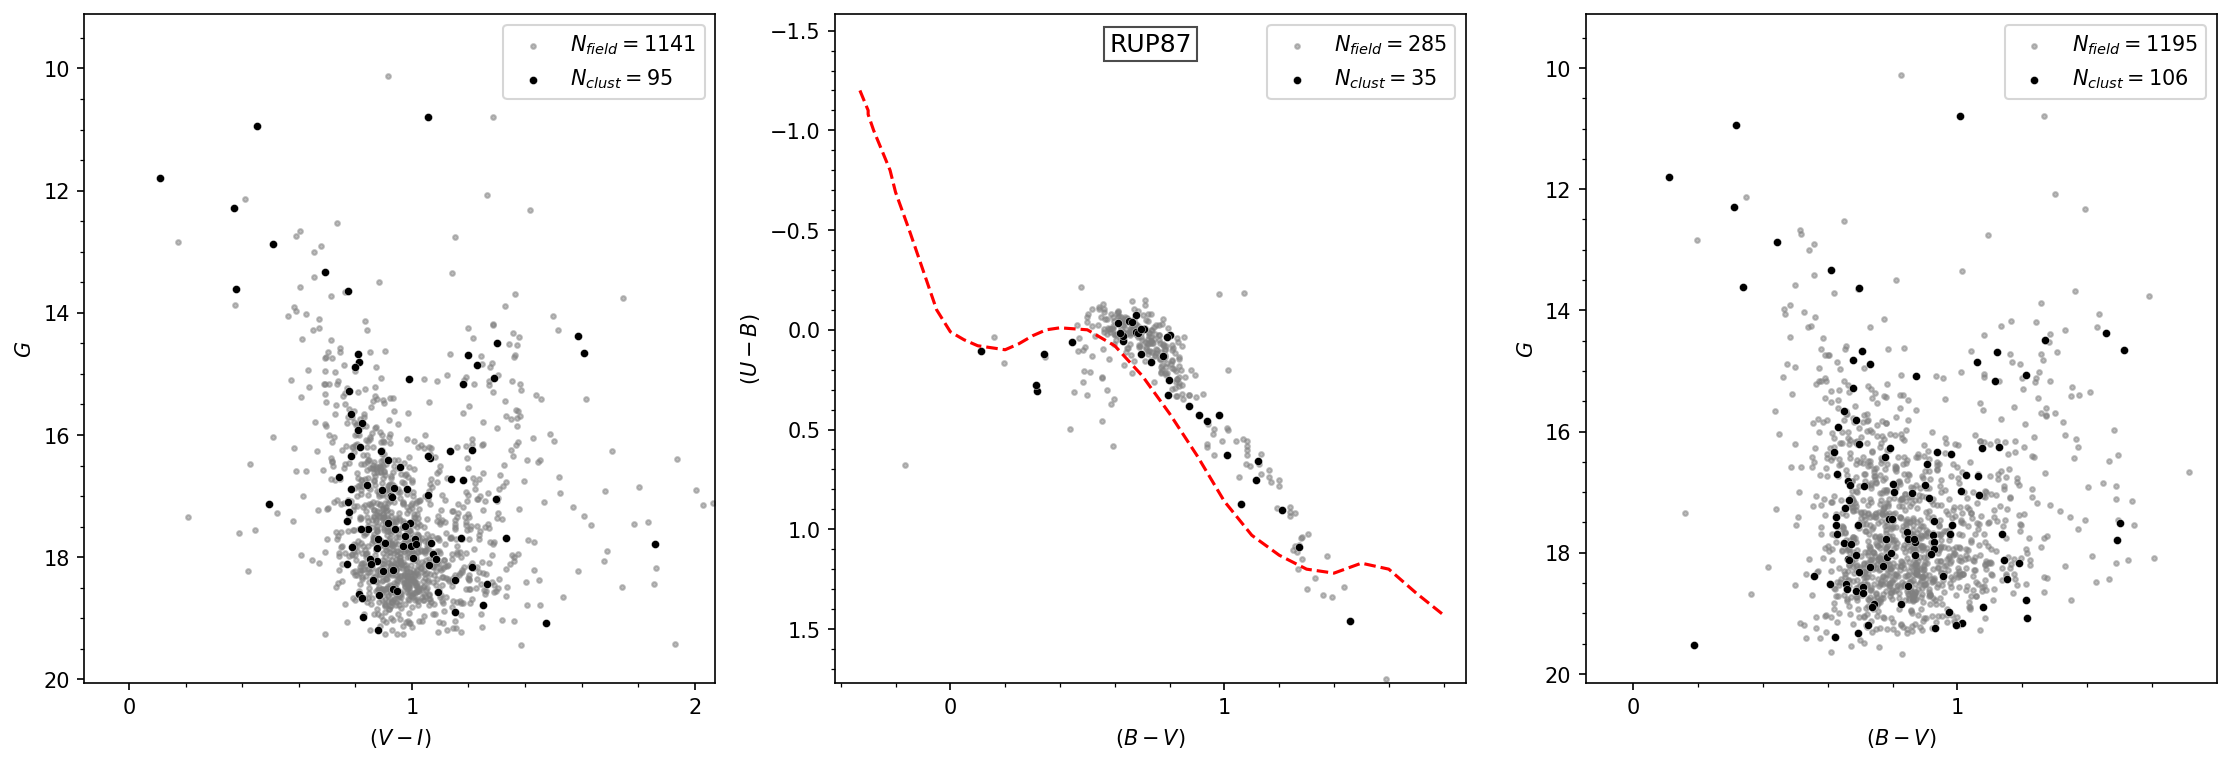
\includegraphics[width=\hsize]{../figs/obs_RUP87.png}
    \caption{Idem Fig. \ref{fig:photom_vdBH85} for RUP 87.}
    \label{fig:photom_RUP87}
\end{figure*}
\begin{figure*}[ht]
    \centering
    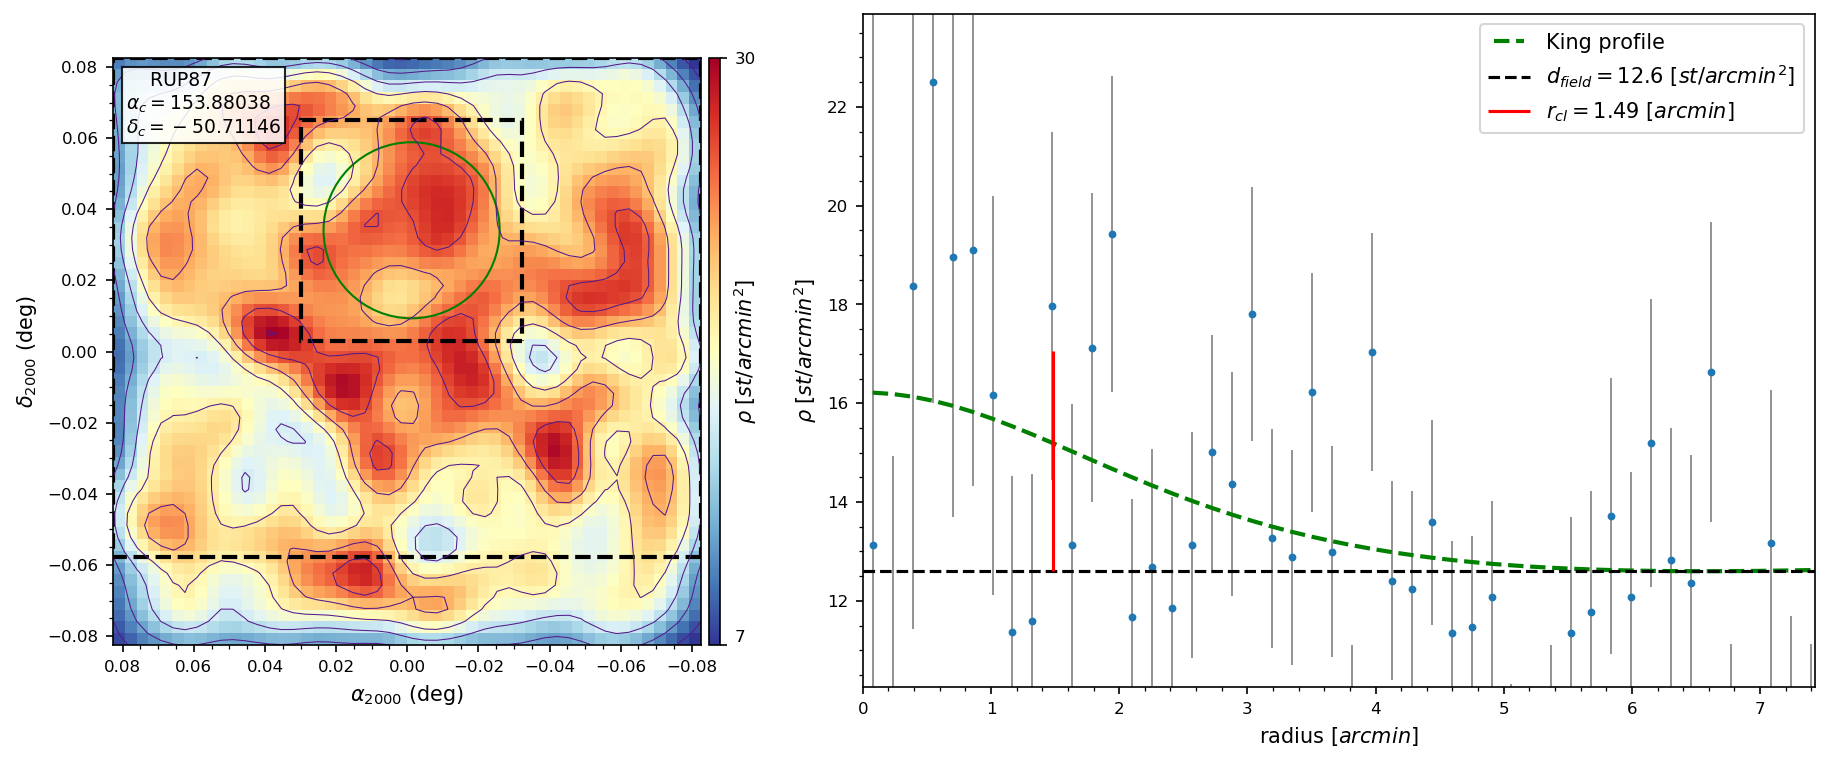
\includegraphics[width=\hsize]{../figs/dmap_rup87.png}
    \caption{Idem Fig. \ref{fig:struct_vdBH85} for RUP 87.}
    \label{fig:struct_RUP87}
\end{figure*}
\begin{figure*}[ht]
    \centering
    \includegraphics[width=\hsize]{../figs/cmds_rup87.png}
    \caption{Idem Fig. \ref{fig:fundpars_vdBH85} for RUP 87.}
    \label{fig:fundpars_RUP87}
\end{figure*}
\begin{figure*}[ht]
    \centering
    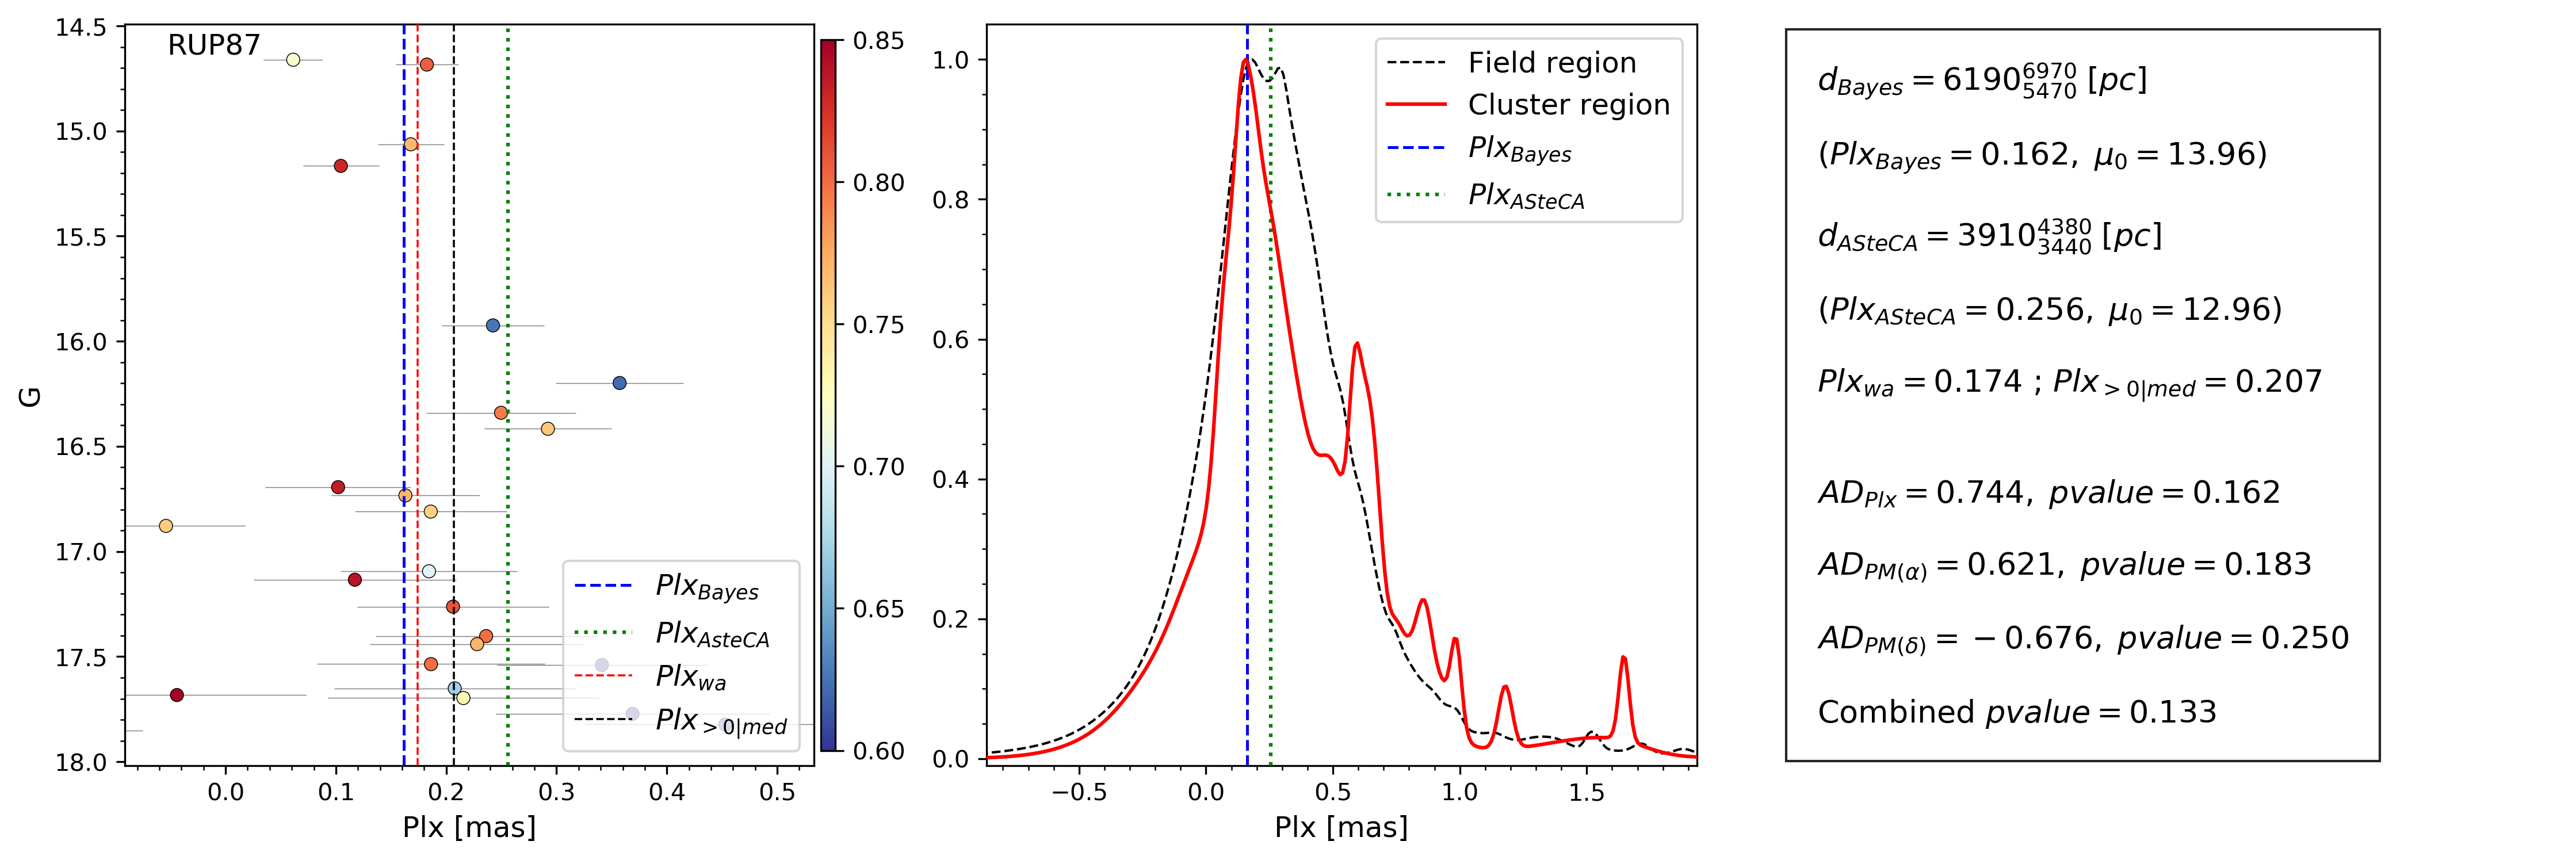
\includegraphics[width=\hsize]{../figs/plx_RUP87.png}
    \caption{Idem Fig. \ref{fig:plx_bys_vdBH85} for RUP 87.}
    \label{fig:plx_bys_RUP87}
\end{figure*}

RUP 87 is located on the east side of the Vela constellation. According to Fig.
\ref{fig:Vim}, there is no relevant feature, but a rather
poorly populated stellar field with a few bright stars
that appear to be grouped  toward the northern portion of the frame.
The photometric diagrams in Fig.~\ref{fig:photom_RUP87} show no appreciable
stellar structure defining the presence of an open cluster.
The few stars with $(U-B)$ measures plotted in the respective CCD
resemble that of a typical Galactic field dominated by a handful of late $F$-
and $G$-type stars followed by a pronounced tail of red stars of presumably
evolved types. Stars in the region $0<(U-B)<0.5$ and $0<(B-V)<0.6$ may be
reddened early $A$- or/and late $B$-type stars.\\

Accordingly, after many trials, \texttt{ASteCA} was not able to \textbf{detect}
an overdensity, as Fig.~\ref{fig:struct_RUP87} clearly shows.
This means that the potential locus occupied by the cluster RUP 87 is not
unambiguously separated from the field background stars.
Lacking a clear overdensity, we define the cluster region as that encircled by
the green line, that is, the sector containing the apparently grouped bright
stars. The RDP emerging from this analysis is quite noisy.

Comparing the density of the defined cluster region with that of the
remaining stellar field, we find that the approximate number of probable
members is 20 stars.
%
When studying (purported) clusters with such a low estimated number of
members, it is important to be extremely careful with the selection of stars
that are considered to be members. If we were to simply select a small group
of stars within a similar parallax range and analyzed their photometric
diagram with \texttt{ASteCA}, we would probably obtain a somewhat reasonable
fit because the code always finds the most likely solution,
regardless of how dispersed the photometric diagram might be. If we a
priori hand-pick a few stars with a common distance (parallax values), they
are fit by a synthetic cluster with a very similar distance modulus as
that defined by the selected parallax values, and some best-fit values
for the remaining parameters.
%
Similarly, the naive selection of stars with probabilities higher than 0.5 is
not appropriate most of the times (unless a clear sequence can
be defined, as in the case of NGC 4349) because this selection is biased
toward brighter stars.
This is because low-mass stars not only have larger associated uncertainties,
they are also located in denser regions of the CMDs. This makes them much more
likely to be assigned lower membership probabilities. A simple cut at 0.5
would generally result in a cluster sequence composed mostly of bright stars,
without respecting the actual photometric density of the purported cluster 
(given by differences in photometric density of the the cluster region versus field region).
%
The stars that are selected within the cluster region should therefore be not only those
with high membership probabilities or share a similar physical attribute 
(i.e., parallax). They should also be properly distributed in the photometric
diagrams and as close as possible in number to the estimated number of members.
As stated above, this is of particular importance for clusters with few members because the process of determining their best-fit parameters is driven by a handful of
stars. This makes the analysis much more delicate.

In the case of RUP 87, we selected stars that had both high membership
values and were similar in number to the estimated number of members for the
cluster region. The 24 stars that remain in the adopted region along with the
best fit are shown in Fig.~\ref{fig:fundpars_RUP87}. The code fits a
somewhat old ($3.1\times10^9$ yr) synthetic cluster at a distance of
$\sim3900$ pc.\\

Figure~\ref{fig:plx_bys_RUP87} shows that the distance estimated through
Gaia parallaxes for the same set of stars is $\sim6200$ pc, which is more
than 2000 pc away from the photometric estimate. This difference is too large to
be consistent with a real cluster, even when possible offsets are taken into account.
We determined whether this discrepancy might be solved as we did for vdBH 85 (see
Sect.~\ref{sec:gaia_distances}), we ran the same analysis with
Bailer-Jones distances. The resulting weighted average for the
distance is $4680_{3090}^{6260}$ pc. This distance is almost 800 pc larger
than the photometric estimate, and 1500 pc smaller than the Gaia parallax
estimate. Large differences like this are consistent with the fact that we did not
analyze an actual cluster.

The Anderson-Darling test values for $Plx$ and proper motions do not confirm
clear differences between the cluster region and the stellar background in
terms of kinematics and distance. The poverty of the photometric diagrams and
the analysis of photometric distances versus parallax distances
are all against the true existence of a cluster in the region RUP 87.
In our interpretation, this is not a real entity, but the fluctuation of the star
field.





%================================================================
\section{Analysis of Gaia parallax distances}
\label{sec:gaia_distances}

We complete our analysis by studying the distances yielded
by \texttt{ASteCA} and those that can be obtained using parallaxes alone.
Specifically, we cross-matched $Plx$ data with our photometry, cluster by
cluster, and processed them within a Bayesian framework (as explained in Sect
\ref{ssec:gaia_data}). The intention is to visualize the change in estimated
distances when no correction is applied to the parallaxes and when current
values taken from the literature are used.\\

In Fig. \ref{fig:prlxbias} we show the \texttt{ASteCA} versus Bayesian 
(parallax) distances with no offset applied (left), and the Bayesian
parallax for each cluster (as the inverse of the distance) versus its
difference with the \texttt{ASteCA} estimate (middle).
%
It is evident from this figure that \texttt{ASteCA} distances are
systematically smaller than those coming from the computation of parallax
alone. The mean of the \texttt{ASteCA} minus parallax differences in
distance is $\sim-411$ pc.
The middle plot with the mean difference suggests that a correction of
+0.028 mas needs to be applied to the Gaia DR2 parallax values.
%
The cluster vdBH85 is omitted from Fig.~\ref{fig:prlxbias} (left and
middle plots) because the Bayesian framework applied on its parallax data
yielded results that were clearly incorrect. This is shown in Fig. 
\ref{fig:plx_bys_vdBH85}, where the estimated parallax distance exceeds 8 kpc compared with the photometric distance obtained by \texttt{ASteCA} of $\sim$4.6 kpc.
Out of the ten clusters in our list of confirmed plus dubious clusters, vdBH85
is the oldest. This means that its main sequence is quite short and
composed mostly of low-mass stars.
More than 60\% of its 146 estimated members have $G>18$ mag, and almost
75\% have Gaia DR2 parallax values with uncertainties larger than 0.1 mas 
(with a mean parallax uncertainty of $\sim$0.16 mas). Because of this, the
Bayesian method fails to estimate a reasonable distance for this cluster,
and we omit it from this analysis.\\

\begin{figure*}[ht]
    \centering
    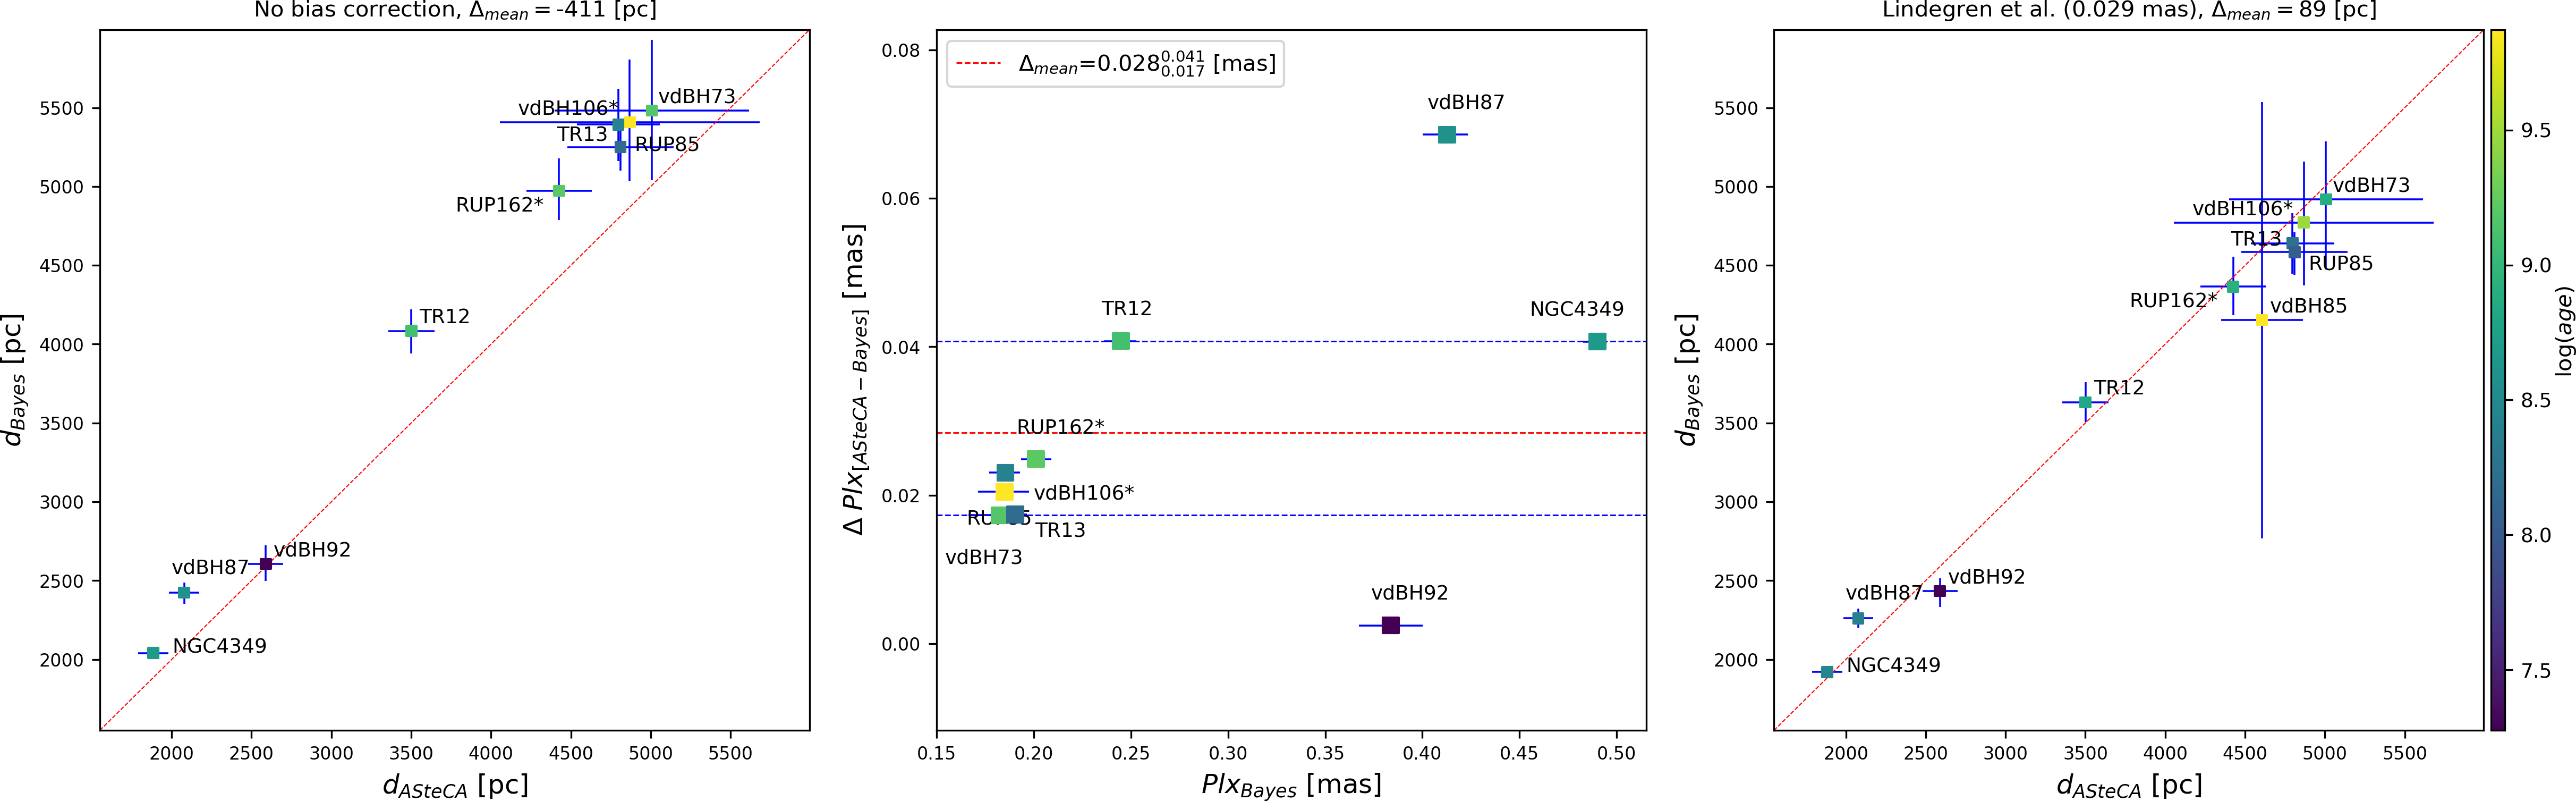
\includegraphics[width=\hsize]{../figs/dist_comparision.png}
\caption{Left: \texttt{ASteCA} (photometric) vs. Bayesian (parallax)
distances for the clusters listed in Table~\ref{tab:final_tab} that are
confirmed to be real clusters. No bias correction was applied to the parallax
data. The color bar at the right indicates $\log(age)$ values.
Center: Offset (\texttt{ASteCA} - Bayes) for distances expressed as
parallax in miliarcseconds.
Right: Same as left plot, with bias corrections from Lindegren et al.
(+0.029 mas).
The cluster vdBH85 is included here; its distance value is estimated from the
list of individual distances reported by \cite{BailerJones_2018}.
}
    \label{fig:prlxbias}
\end{figure*}

A number of recent articles have found an offset in the
Gaia parallax data that covers a range of approximately +0.05 mas. We selected
three of these articles that fully cover this range to compare them with our
results, which were obtained with no bias corrections: \cite{Lindegren_2018},
\cite{Schonrich2019}, and \cite{Xu_2019}.
%
Lindegren et al. processed the parallax of hundreds of
thousands of quasars and derived a median difference with Gaia data of +0.029 mas. Sch\"onrich et al. analyzed the radial velocity subset of Gaia
DR2 with their own Bayesian inference tool and estimated a required +0.054 mas
offset in the parallax data from Gaia DR2. Finally, Xu et al. used $\sim$100
stars with VLBI astrometry and found an offset of
+0.075 mas with Gaia DR2 parallaxes. 
%
When we add the offsets given in Lindegren et al., 
Sch\"onrich et al., and Xu et al. (+0.029, +0.054, +0.075 mas,
respectively) to the parallax data, the agreement between \texttt{ASteCA} and the parallax distances
improves at first and then rapidly worsens. The mean differences between photometric
distances and parallax distances are $\sim0.09$ kpc, $\sim0.39$ kpc, and
$\sim0.62$ kpc, using the Lindegren et al., Sch\"onrich et al., and Xu
et al. corrections, respectively.

We are unable to apply the Bayesian method described in
Sect.~\ref{ssec:gaia_data} (as explained above) to vdBH85,
therefore we considered the individual distance values obtained in
\cite{BailerJones_2018}.
The authors used Bayesian inference to estimate distances (in
parsec) to more than one billion stars using the Gaia DR2 parallax values by
applying the correction reported by Lindegren et al..\footnote{This is not to be
confused with the Bayesian inference method described in
Sect.~\ref{ssec:gaia_data}. These are two very different processes.}
We cross-matched our list of members for vdBH85 and approximated the distance to
the cluster as their average distance, weighted by the assigned uncertainties.
Although this is a rather low-quality estimate because of the large
uncertainties in the individual distances, as seen by the large error bars
in Fig. \ref{fig:prlxbias} (right plot), it is still close to the
photometric distance estimate.
When we omit vdBH85 entirely, the Lindegren et al. mean difference improves to
$\sim0.05$ kpc.

Our analysis thus indicates a required bias correction to Gaia parallaxes of
+0.028 mas, which is very close to the value proposed by Lindegren et al.\\

In Sect \ref{ssec:photom_reduc} we described that our $(B-V)$ color has a small
offset of $\sim0.0153$ mag when compared to the (transformed) Gaia photometry.
\texttt{ASteCA} employs the extinction law by \citet[][CCC law]{Cardelli_1989}
with the \citet{Odonnell_1994} correction for the near-UV, to transform $E
(B-V)$ values into absorptions for any filter.
In our case, we used the Gaia $G$ filter, whose absorption $A_G$ is related to $E
(B-V)$ as $A_G = c_0 \, A_V  = c_0 \, 3.1 \, E(B-V)$, where $c_0\approx0.829$
according to the CCC law. The absorption $A_{G}^{\prime}$, that is,
corrected for the offset in $(B-V)$, can accordingly be written as $A_{G}^
{\prime}=0.039+A_G$.
For the range of distance moduli in this work ($\sim$11 - 14 mag), the effect
of this correction on the distance in parsec extends from $\sim$30 to 100 pc.
When we applied this $(B-V)$ offset to our photometric distances and repeated the
analysis, the +0.028 mas bias in Gaia parallaxes that we found
initially was reduced to +0.023 mas. This is a lower value, but still very
close to the bias reported by Lindegren et al.

An analysis of a more extended sample of clusters is certainly needed for conclusive results and to establish the detailed relation between
distances from photometry and DR2 parallaxes. The results of the exercise
presented in this section are included in the last four columns of Table 
\ref{tab:final_tab}.




%================================================================
\section{Discussion of results and concluding remarks}
\label{sec:results_concl}

We have analyzed the fields of 16 cataloged open clusters located in a
Galaxy sector covering approximately $270^\circ$ to $300^\circ$  in
Galactic longitude, and mostly close to the formal Galactic plane at
$b=0^\circ$.
The cluster parameter estimates presented in this article are based on
precise $UBVI$ photometry analyzed in a automatic way by our code 
\texttt{ASteCA}. The code searches for a meaningful stellar overdensity
and assigns membership probabilities by comparison with the surrounding stellar
field.
The next step establishes the physical properties of the best synthetic cluster
that fits the distribution of cluster members in the CMDs and the CCD.
Through this process, reddening, distance, age, mass, and metallicity are
given.
The most relevant inconvenience we have found with this cluster
sample is that some of the clusters are extremely faint, which
becomes evident in a visual inspection of their overall CCDs and CMDs.
This becomes more difficult because the $(U-B)$ index has mostly been available
only for the bright and blue stars. This considerably reduced the data analysis
space. Despite this, we were able to control the reddening solutions
and obtained reliable distance estimates for the objects that were found to be 
true clusters by our code. In this way, we can safely reject RUP 87, vdBH91,
RUP 88, Lynga 15, Loden 565, and NGC 4230, which most probably are random
stellar fluctuations. The results for true and probable open clusters are shown
in Table~\ref{tab:final_tab} in a self-explaining format.

\begin{table*}[ht]
\small
\centering
\caption{\textbf{Fundamental parameters and parallax distances obtained for
the confirmed and probable clusters}. The asterisk indicates probable clusters.
The $d_{noofset}$ values are those obtained using the Bayesian method without
bias correction  on the Gaia DR2 parallax data. The remaining distances were
obtained by applying the indicated offsets to the parallax values.}
\begin{tabular}{lccccccccc}
\hline \hline 
 \emph{Cluster} & z & \emph{Age} & $E(B-V)$ & \emph{Mass} &
 $d_{ASteCA}$ & $d_{noofset}$ & $d_{Lindegren}$ & $d_{Sch\ddot{o}nrich}$ &
 $d_{Xu}$ \\
& & $(10^9 yr)$ & $mag$ & $(10^3\,M_{\odot})$ & $(kpc)$ & $(kpc)$ & $(kpc)$ &
$(kpc)$ & $(kpc)$\\
 \hline
 vdBH 73 & 0.019$\pm0.004$ & 0.78$\pm0.09$ & 1.06$\pm0.04$ & 2.6$\pm0.9$ &
  $5.01\pm0.61$ & $5.48\pm0.44$ & $4.92\pm0.41$ & $4.46\pm0.31$ & $4.05\pm0.33$\\
 %
 RUP 85 & 0.021$\pm0.003$ & 0.18$\pm0.03$ & 1.06$\pm0.03$ & 2.6$\pm0.5$ &
 $4.80\pm0.26$ & $5.39\pm0.23$ & $4.64\pm0.19$ & $4.16\pm0.15$ & $3.83\pm0.14$\\
 %
 vdBH 85 & 0.014$\pm0.002$ & 7.50$\pm0.80$ & 0.30$\pm0.03$ & 2.2$\pm0.5$ &
  $4.61\pm0.26$ & -- & $4.15\pm1.38$ & -- & --\\
 %
 vdBH 87 & 0.025$\pm0.002$ & 0.25$\pm0.08$ & 0.55$\pm0.04$ & 1.4$\pm0.2$ &
 $2.08\pm0.09$ & $2.42\pm0.07$ & $2.26\pm0.06$ & $2.13\pm0.05$ & $2.05\pm0.05$\\
%
 TR 12 & 0.009$\pm0.002$ & 0.70$\pm0.10$ & 0.31$\pm0.03$ & 0.7$\pm0.1$ &
 %3.50$\pm0.20$ & 4.10$\pm0.10$ & 3.60$\pm$0.10 & 3.30$\pm$0.10 & 3.11$\pm$0.09\\
 $3.50\pm0.15$ & $4.08\pm0.14$ & $3.63\pm0.13$ & $3.31\pm0.10$ & $3.11\pm0.09$\\
 %
 vdBH 92 & 0.009$\pm0.004$ & 0.02$\pm0.01$ & 0.65$\pm0.03$ & 0.4$\pm0.1$ &
 % 2.60$\pm0.10$ & 2.60$\pm0.10$ & 2.43$\pm$0.09 & 2.28$\pm$0.07 & 2.17$\pm$0.07\\
 $2.59\pm0.11$ & $2.61\pm0.11$ & $2.43\pm0.09$ & $2.28\pm0.07$ & $2.17\pm0.07$\\
 %
 TR 13 & 0.007$\pm0.004$ & 0.11$\pm0.02$ & 0.56$\pm0.02$ & 0.7$\pm0.2$ &
 % 4.80$\pm0.30$ & 5.30$\pm$0.20 & 4.60$\pm$0.10 & 4.10$\pm$0.10 & 3.75$\pm$0.09\\
 $4.81\pm0.33$ & $5.25\pm0.16$ & $4.58\pm0.14$ & $4.10\pm0.11$ & $3.75\pm0.09$\\
 %
 vdBH 106* & 0.012$\pm0.003$ & 3.00$\pm0.80$ & 0.30$\pm0.04$ & 0.5$\pm0.2$ &
 % 4.90$\pm$0.80 & 5.40$\pm$0.40 & 4.80$\pm$0.40 & 4.30$\pm$0.30 & 4.10$\pm$0.30\\
 $4.87\pm0.81$ & $5.41\pm0.39$ & $4.77\pm0.39$ & $4.31\pm0.33$ & $4.06\pm0.30$\\
 %
 RUP 162* & 0.009$\pm0.002$ & 0.80$\pm0.20$ & 0.54$\pm0.03$ & 1.2$\pm0.2$ &
 % 4.40$\pm$0.20 & 5.00$\pm$0.20 & 4.40$\pm$0.20 & 3.90$\pm$0.20 & 3.70$\pm$0.10\\
 $4.43\pm0.20$ & $4.97\pm0.20$ & $4.37\pm0.18$ & $3.94\pm0.15$ & $3.66\pm0.13$\\
 %
 NGC 4349 & 0.011$\pm0.004$ & 0.29$\pm0.09$ & 0.41$\pm0.05$ & 2.0$\pm0.1$ &
 $1.88\pm0.05$ & $2.04\pm0.03$ & $1.92\pm0.02$ & $1.83\pm0.02$ & $1.76\pm0.01$\\
\hline
\end{tabular}
\label{tab:final_tab}
\end{table*}

When we average the metallicity for each cluster, shown in the second
column of Table \ref{tab:final_tab}, the metal content is $z=0.0136\pm0.006$.
The result agrees well with the assumption that the typical  open cluster in the Milky Way has solar metallicity \citep[$z=0.0152$,][]{Bressan_2012}.\\

Of the remaining ten objects, two are probable clusters with distances in the
4-5 kpc range. The cluster ages range from a few million years
to almost 8 billion years in the case of vdBH 85. The vdBH 106 cluster
is one of the oldest, but it is just a probable open cluster, therefore its age needs
be taken with caution. Two other objects, TR 13 and vdBH 92, are young, with
ages close to and younger than 100 million years, respectively, and the remaining are all
younger than 1 billion years.

A final remark concerns the spatial distribution of the
eight real and two probable clusters listed in Table 
\ref{tab:final_tab}. These objects  are plotted in Fig~\ref{fig68} in the X-Y
(upper) and X-Z (lower) planes of the Milky Way, following the usual sign
convention. The Sun is placed at $(0, 0)$. Superposed is the outline of the
Carina Arm, taken from \cite{valle_2005}. All these objects are plotted with
open circles except, for the two youngest, which are shown with red squares. TR
13, one of the youngest (0.1 Gyr) and farthest (4.8 kpc) objects, is located at
the external side of the Carina arm but appears well below the Galaxy plane at
about -0.2 kpc. This means that it follows the warp of this arm, which has been
mentioned among others by \cite{Cersosimo_2009}.
The other young cluster, vdBH 92 (0.02 Gyr), is relatively far from the nucleus
of the Carina Nebula in an intermediate zone between that region and the Sun,
but is still seen close to the northwest side of the Carina Nebula at a
distance that lies within the estimated maximum and minimum distance for
Carina.
vdBH 106 (3 Gyr) and vdBH 85 (7.5 Gyr) are the oldest objects in our
search and are in turn placed well above the formal Galactic equator (0.3-0.4
kpc). TR 12 (0.7 Gyr) is another quite old object that is placed below the plane (-0.2
kpc) together with RUP 162 (1 Gyr). The remaining clusters are of middle age
and lie relatively closely to the Galaxy plane.

We conclude for the photometric versus parallax distances that by
adding $\sim+0.028$ mas to the computed cluster parallaxes from Gaia DR2,
the level of agreement with the photometric distances improves considerably.
When the small offset found for the $(B-V)$ color is taken into account, this
value drops to +0.023 mas, which is only 0.006 mas lower than the correction applied by
Lindegren et al., +0.029 mas.
This supports the evidence that indicated this offset over higher
values proposed in the literature. Our cluster sample is not large enough
to permit drawing stronger conclusions on this matter, particularly
regarding the possible dependence of the correction on distance.


\begin{figure}[ht]
    \centering
    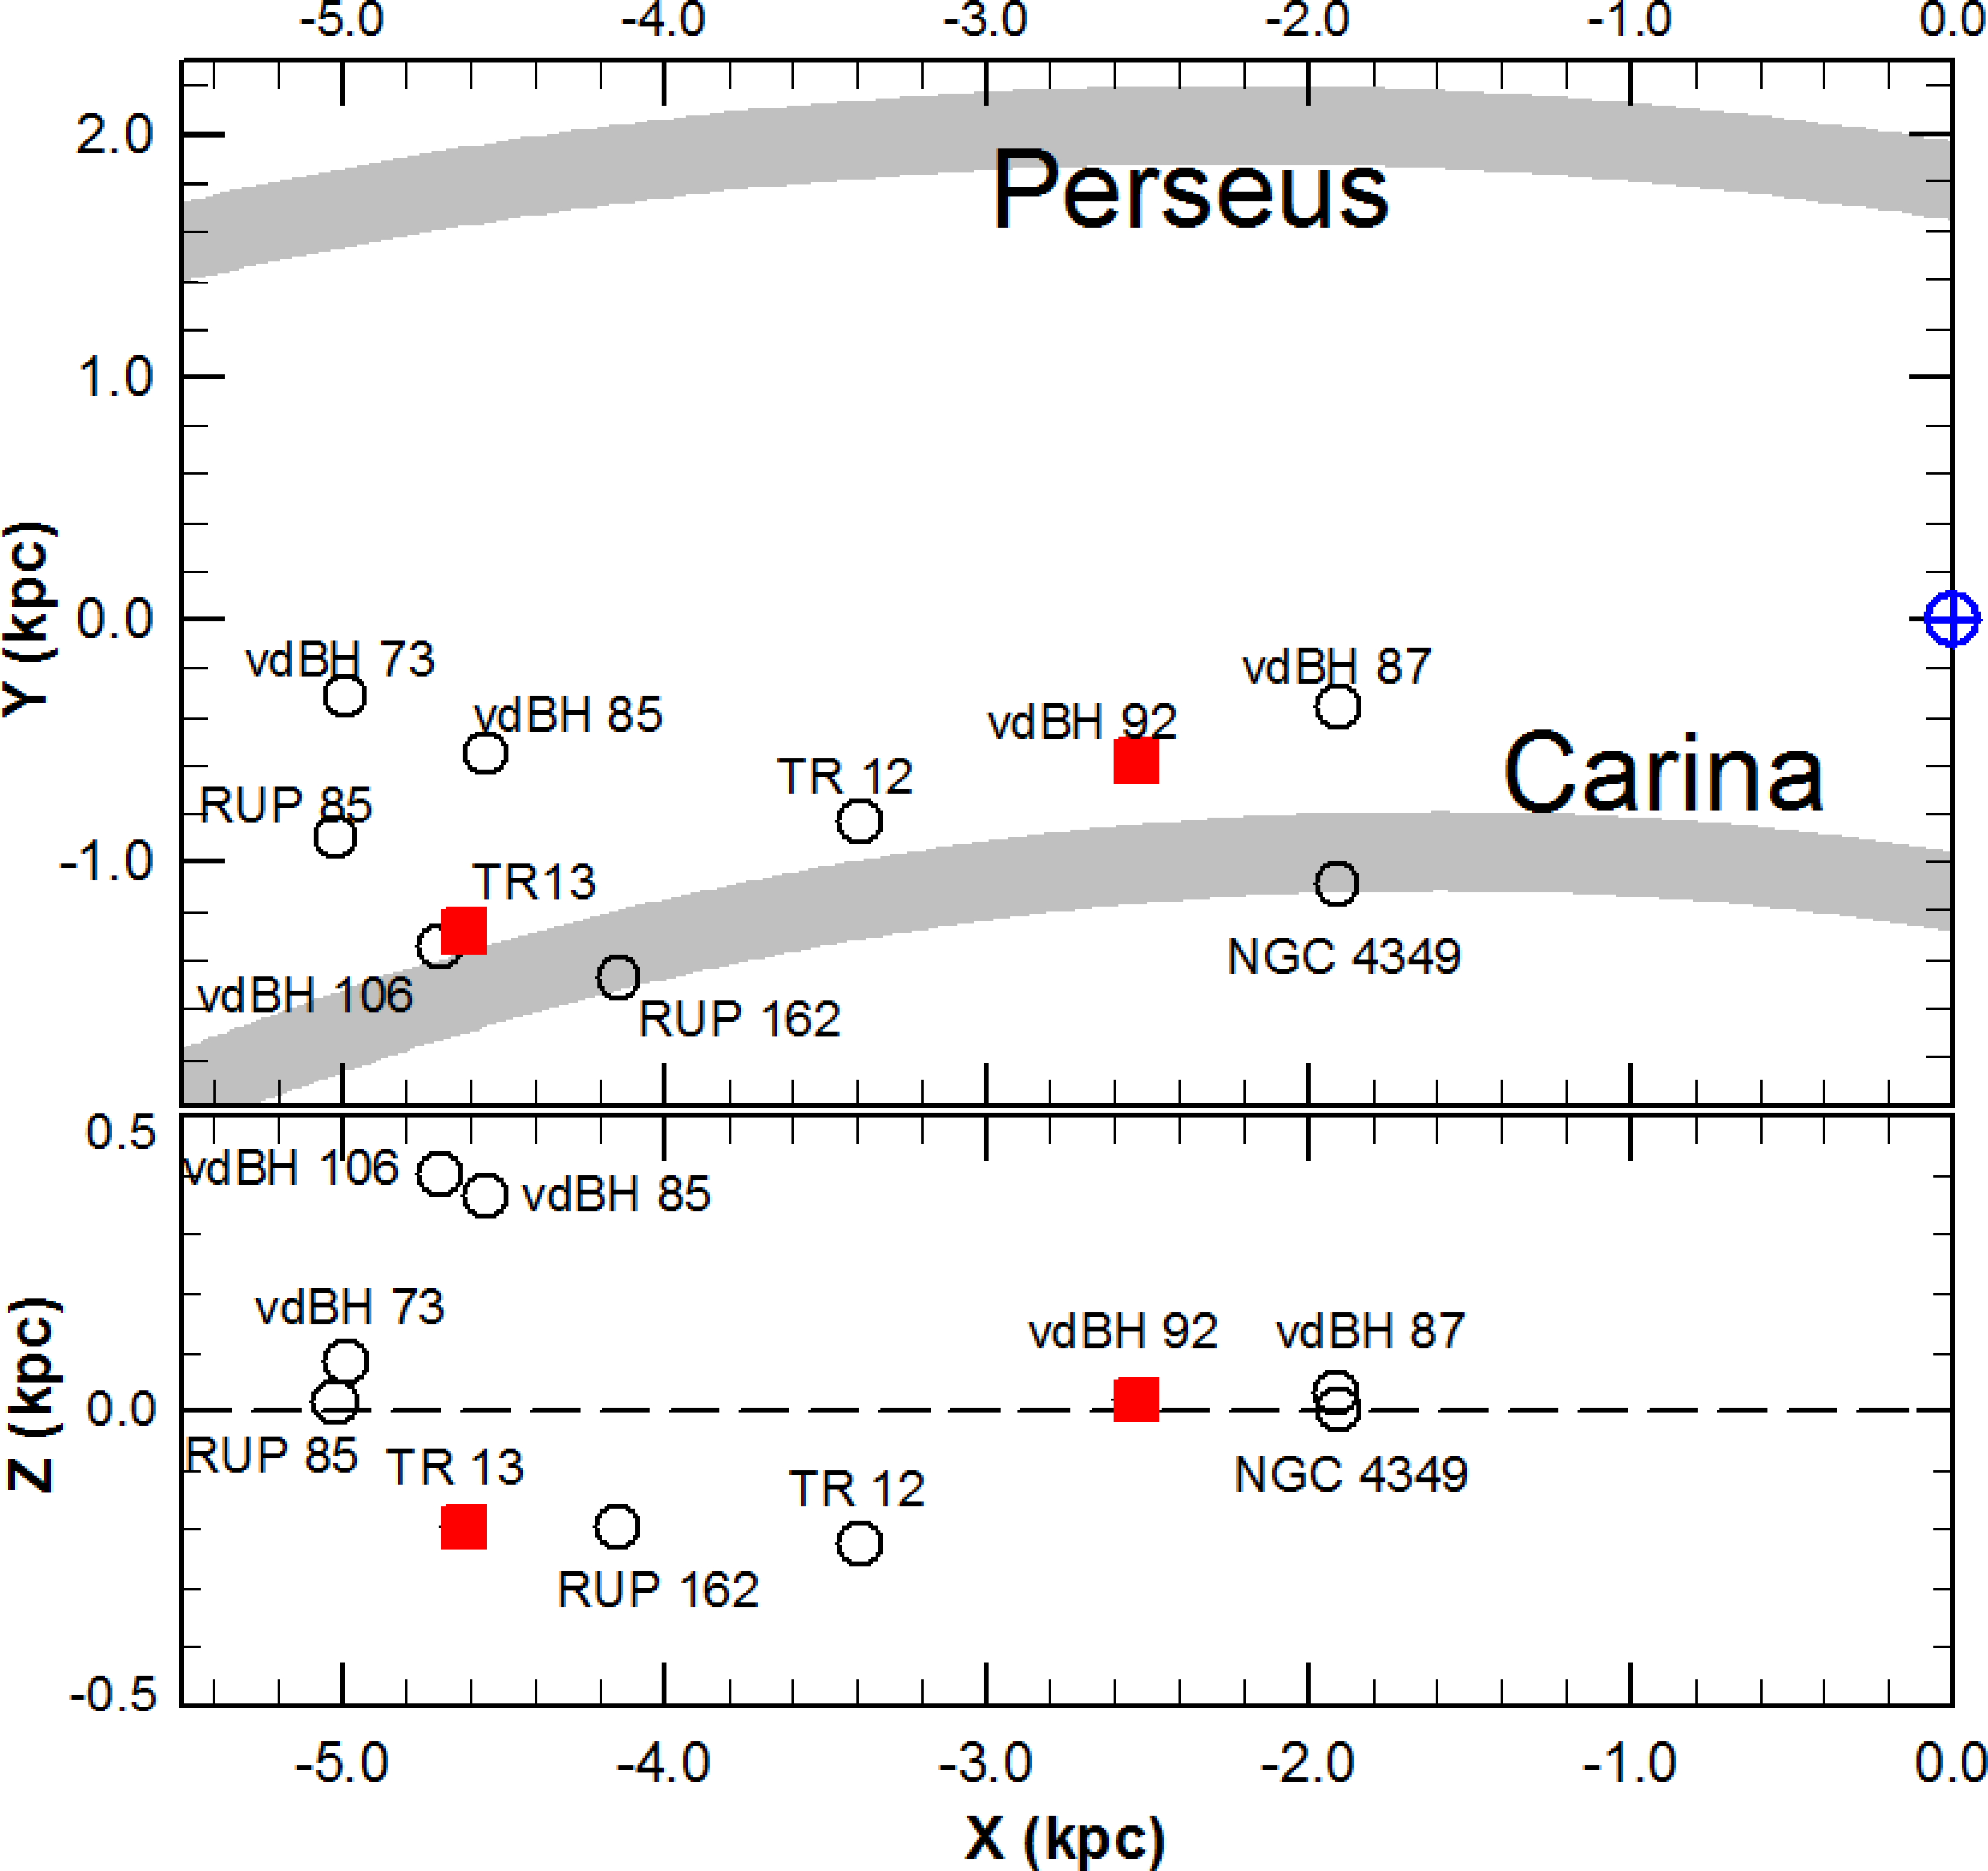
\includegraphics[width=\hsize]{../figs/xy_xz.png}
\caption{X-Y (upper panel) and X-Z (lower plane) projection of the true and
probable clusters in our sample (open circles). The red squares
enclose the youngest clusters in our list (see Table~\ref{tab:final_tab}).
The thick gray lines in the upper panel show the trace of the Perseus and
Carina arms according to \cite{valle_2005}.
The position of the Sun is shown by a blue crossed circle.
The dashed line in the lower panel depicts the Galactic equator.}
\label{fig68}
\end{figure}


\begin{acknowledgements}

G.P., E.E.G., M.S.P. and R.A.V. acknowledge the financial support from CONICET 
(PIP317) and the UNLP.
AM acknowledges the support from the Portuguese Strategic Programme
UID/FIS/00099/2019 for CENTRA.
The authors are very much indebted with the anonymous referee for the helpful
comments and suggestions that contributed to greatly improving the manuscript.
%
This research was made possible through the use of the AAVSO Photometric
All-Sky Survey (APASS), funded by the Robert Martin Ayers Sciences Fund and NSF
AST-1412587.
%
This research has made use of the WEBDA database, operated at the Department of
Theoretical Physics and Astrophysics of the Masaryk University.
%
This research has made use of the VizieR catalog access tool, operated at CDS,
Strasbourg, France~\citep{Ochsenbein_2000}.
%
This research has made use of ``Aladin sky atlas'' developed at
CDS, Strasbourg Observatory, France~\citep{Bonnarel2000,Boch2014}.
%
This research has made use of NASA's Astrophysics Data System.
%
This research made use of the Python language v3.7.3~\citep{vanRossum_1995}
and the following packages:
NumPy\footnote{\url{http://www.numpy.org/}}~\citep{vanDerWalt_2011};
SciPy\footnote{\url{http://www.scipy.org/}}~\citep{Jones_2001};
Astropy\footnote{\url{http://www.astropy.org/}}, a community-developed core
Python package for Astronomy \citep{Astropy_2013};
matplotlib\footnote{\url{http://matplotlib.org/}}~\citep{hunter_2007};
emcee\footnote{\url{http://emcee.readthedocs.io}}~\citep{emcee};
corner.py\footnote{\url{https://corner.readthedocs.io}}~\citep{corner}.
\end{acknowledgements}

\bibliographystyle{aa}
\bibliography{biblio}


















































\appendix

The 13 clusters in this appendix are ordered according to their
longitude, as shown in Table \ref{tab:clust_list}. The remaining 3
analyzed clusters were presented in Sect. \ref{sec:cluster_discuss}.


%================================================================
\section{van den Bergh-Hagen 73}

The cluster vdBH 73 is placed in almost the center of the Vela
constellation well at the northeast border of the Carina constellation. The
visual chart of the region in Fig. \ref{fig:Vim} shows a small and compact
grouping of stars at the very center of the frame, surrounded by a dense stellar
field.
The inspection of the CCD and CMDs for all the stars observed
in the targeted region in Fig. \ref{fig:photom_vdBH73} gives no clear
indications about a cluster there, likely because of the field stellar contamination.
A few stars in the CMDs of Fig.~\ref{fig:photom_vdBH73} are above $G=15$
mag, and at higher magnitudes, the CMDs strongly widen.
The reddening in the CCD in the right panel in Fig. \ref{fig:photom_vdBH73} is quite
strong and displaces the bulk of stars entirely toward the red side. A
few blue stars with negative $(U-B)$ values appear to be strongly affected by
variable reddening.\\

The left panel in Fig.~\ref{fig:struct_vdBH73} shows a pronounced stellar
overdensity of 2.2 arcmin radius, coincident with the location expected for
vdBH 73. This overdensity appears to be immersed in a region of large field
stellar contamination. As shown in the RDP to the right, the density peak is about
four times above the mean for the field.\\

The CMDs in Fig.~\ref{fig:fundpars_vdBH73}, left and right panels, show a cluster main sequence subtending 1.5 magnitudes and a faint giant
branch with stars up to $G=15$ mag.
The $(B-V)$ versus $(V-I)$ CCD is shown in the middle panel instead of the
$(B-V)$ versus $(U-B)$ diagram because the latter did not contain enough stars to
be of use in the extinction estimation process.
Although the CMDs after the removal of interlopers look somewhat noisy, stars with membership probabilities above $\sim0.7$ clearly
trace the sequence of an evolved cluster.
The best-fit of a synthetic cluster yields the following results:

\begin{itemize}
\item [a)] The cluster is immersed in a region of moderate absorption
because the mean of the reddening is $E(B-V)=1.06$, which is compatible
with those provided by S\&F2011, who found a maximum $E(B-V)$ of about 1.2 mag
toward vdBH 73.
\item [b)] The absorption-free distance modulus is
$13.50\pm0.26$ mag, placing this object at $5.01\pm0.61$ kpc from the Sun.
\end{itemize}

From the photometric point of view, the existence of a well-outlined cluster main
sequence and the high probability memberships of the stars confirm
the real entity of vdBH 73.
The usage of parallax data from Gaia shows a good agreement in distance,
reaching up $5.48\pm0.44$ kpc in the sense that Gaia parallaxes place the
cluster farther than photometry does. This difference improves when an offset is
applied to the parallax data, as shown in Sect. \ref{sec:results_concl}.
The Anderson-Darling test applied to parallax and proper motion data
demonstrates that the null hypothesis can indeed be rejected with a
combined $p$-value of 0.0. This means that a real cluster is present in this
region.\\

We conclude from our analysis that van den Bergh-Hagen 73 is an intermediate-age cluster that is about $0.78\pm0.09\times10^9$ years old.


\begin{figure*}[ht]
    \centering
    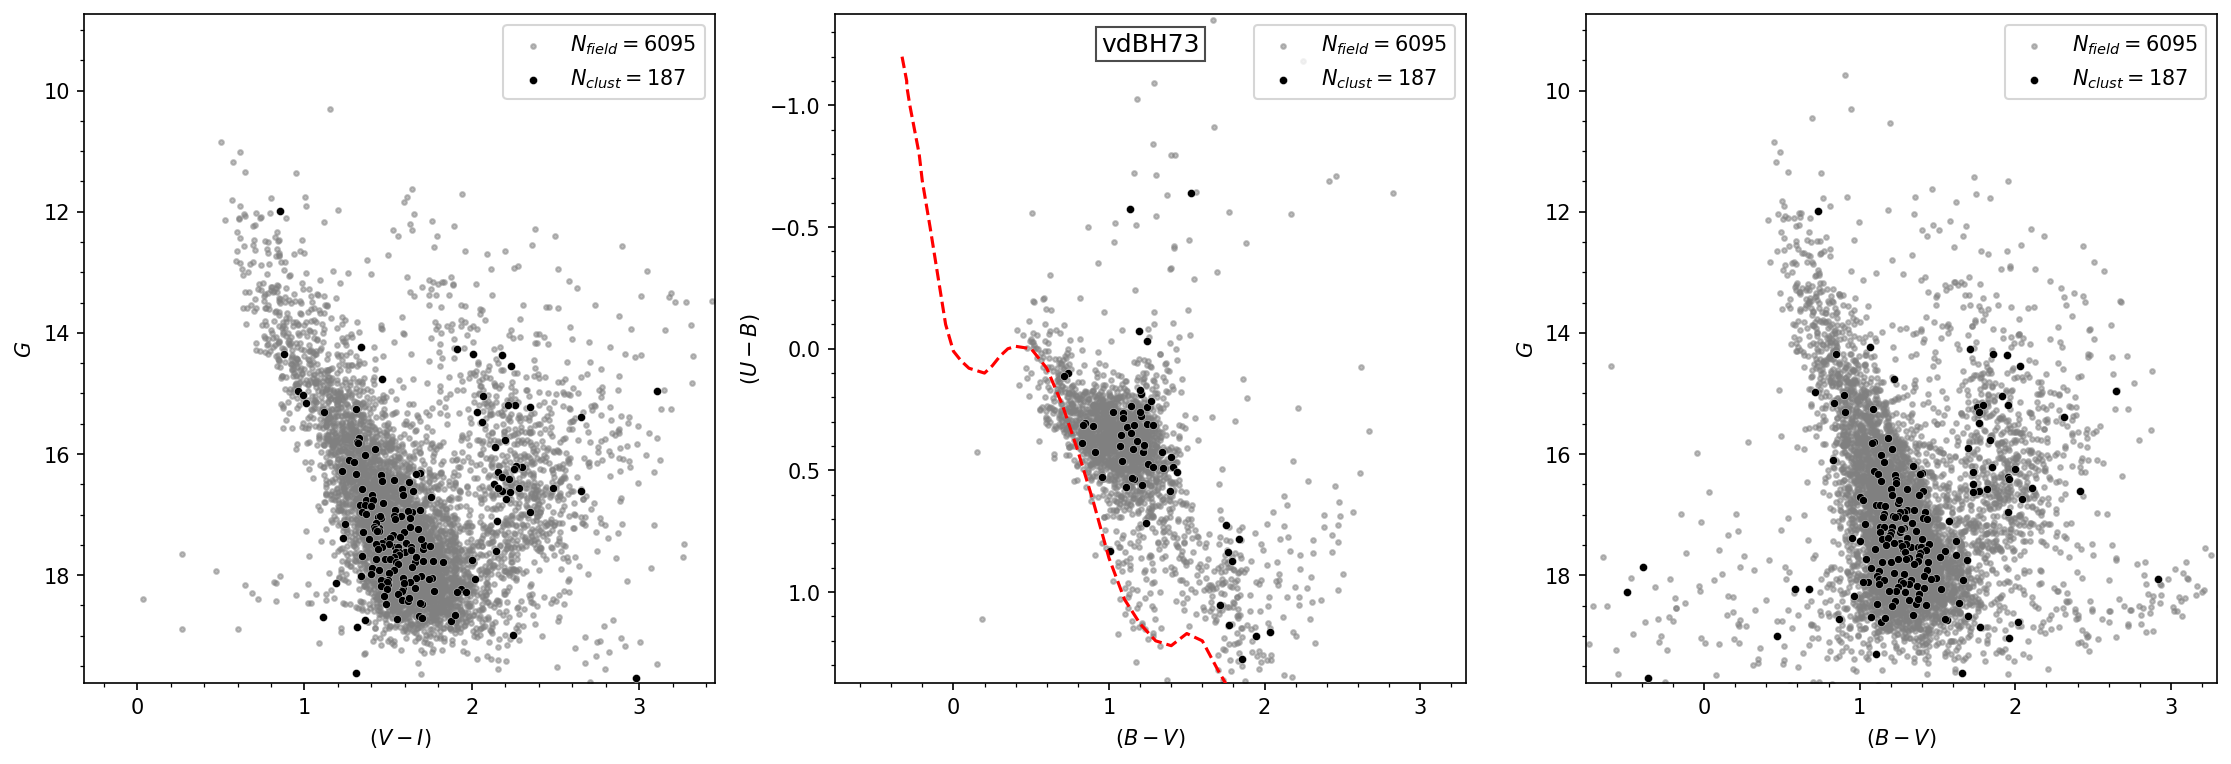
\includegraphics[width=\hsize]{../figs/obs_vdBH73.png}
\caption{Idem Fig. \ref{fig:photom_vdBH85} for vdBH 73.}
    \label{fig:photom_vdBH73}
\end{figure*}

\begin{figure*}[ht]
    \centering
    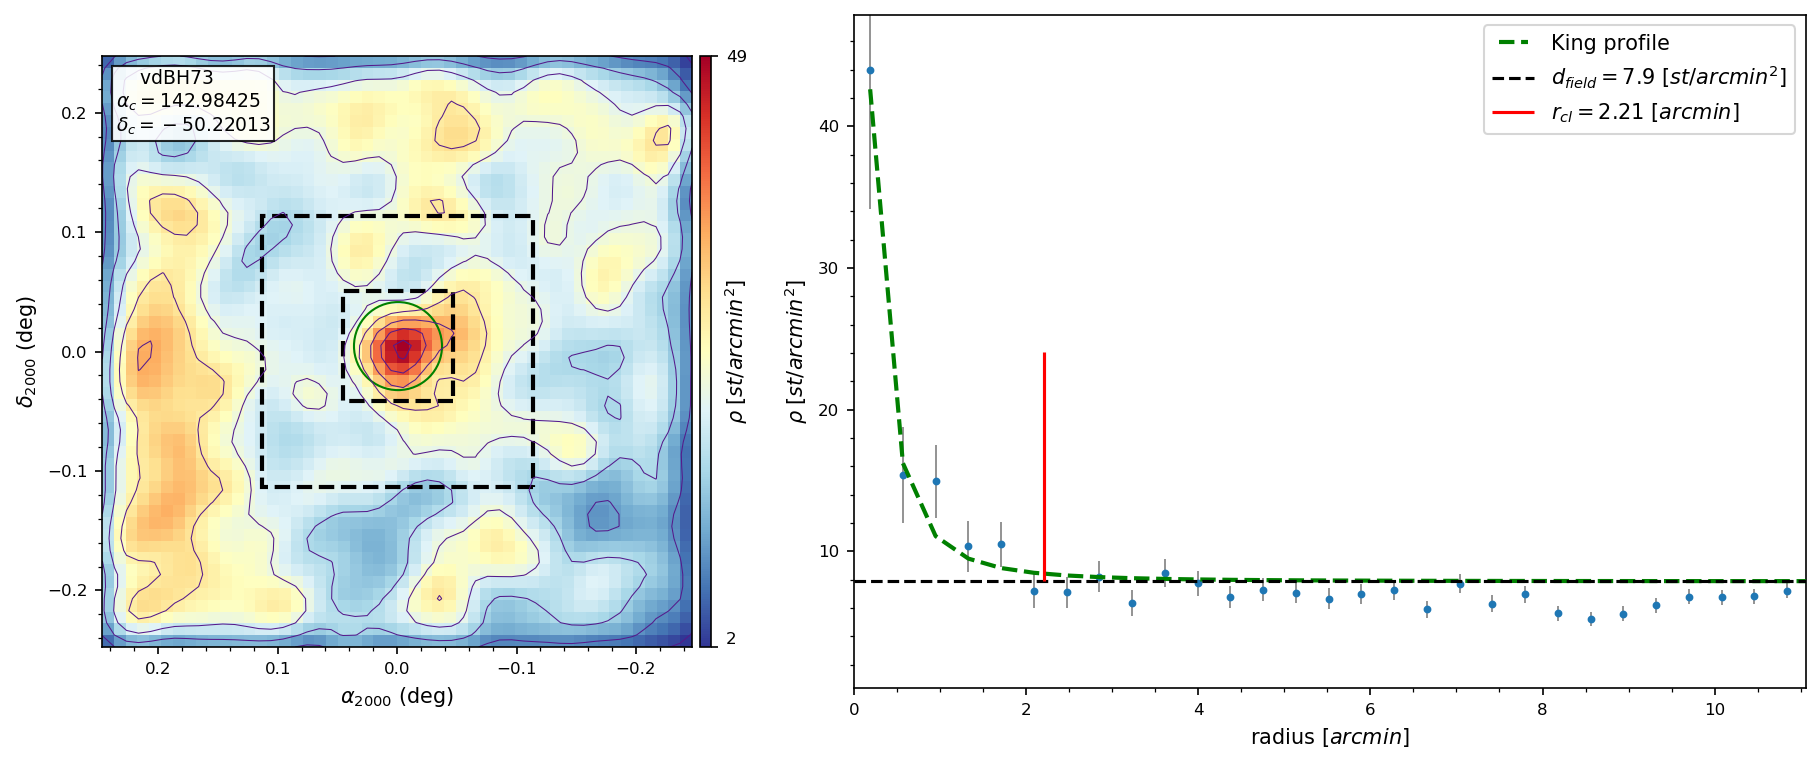
\includegraphics[width=\hsize]{../figs/dmap_vdbh73.png}
\caption{Idem Fig. \ref{fig:struct_vdBH85} for vdBH 73.}
    \label{fig:struct_vdBH73}
\end{figure*}

\begin{figure*}[ht]
    \centering
    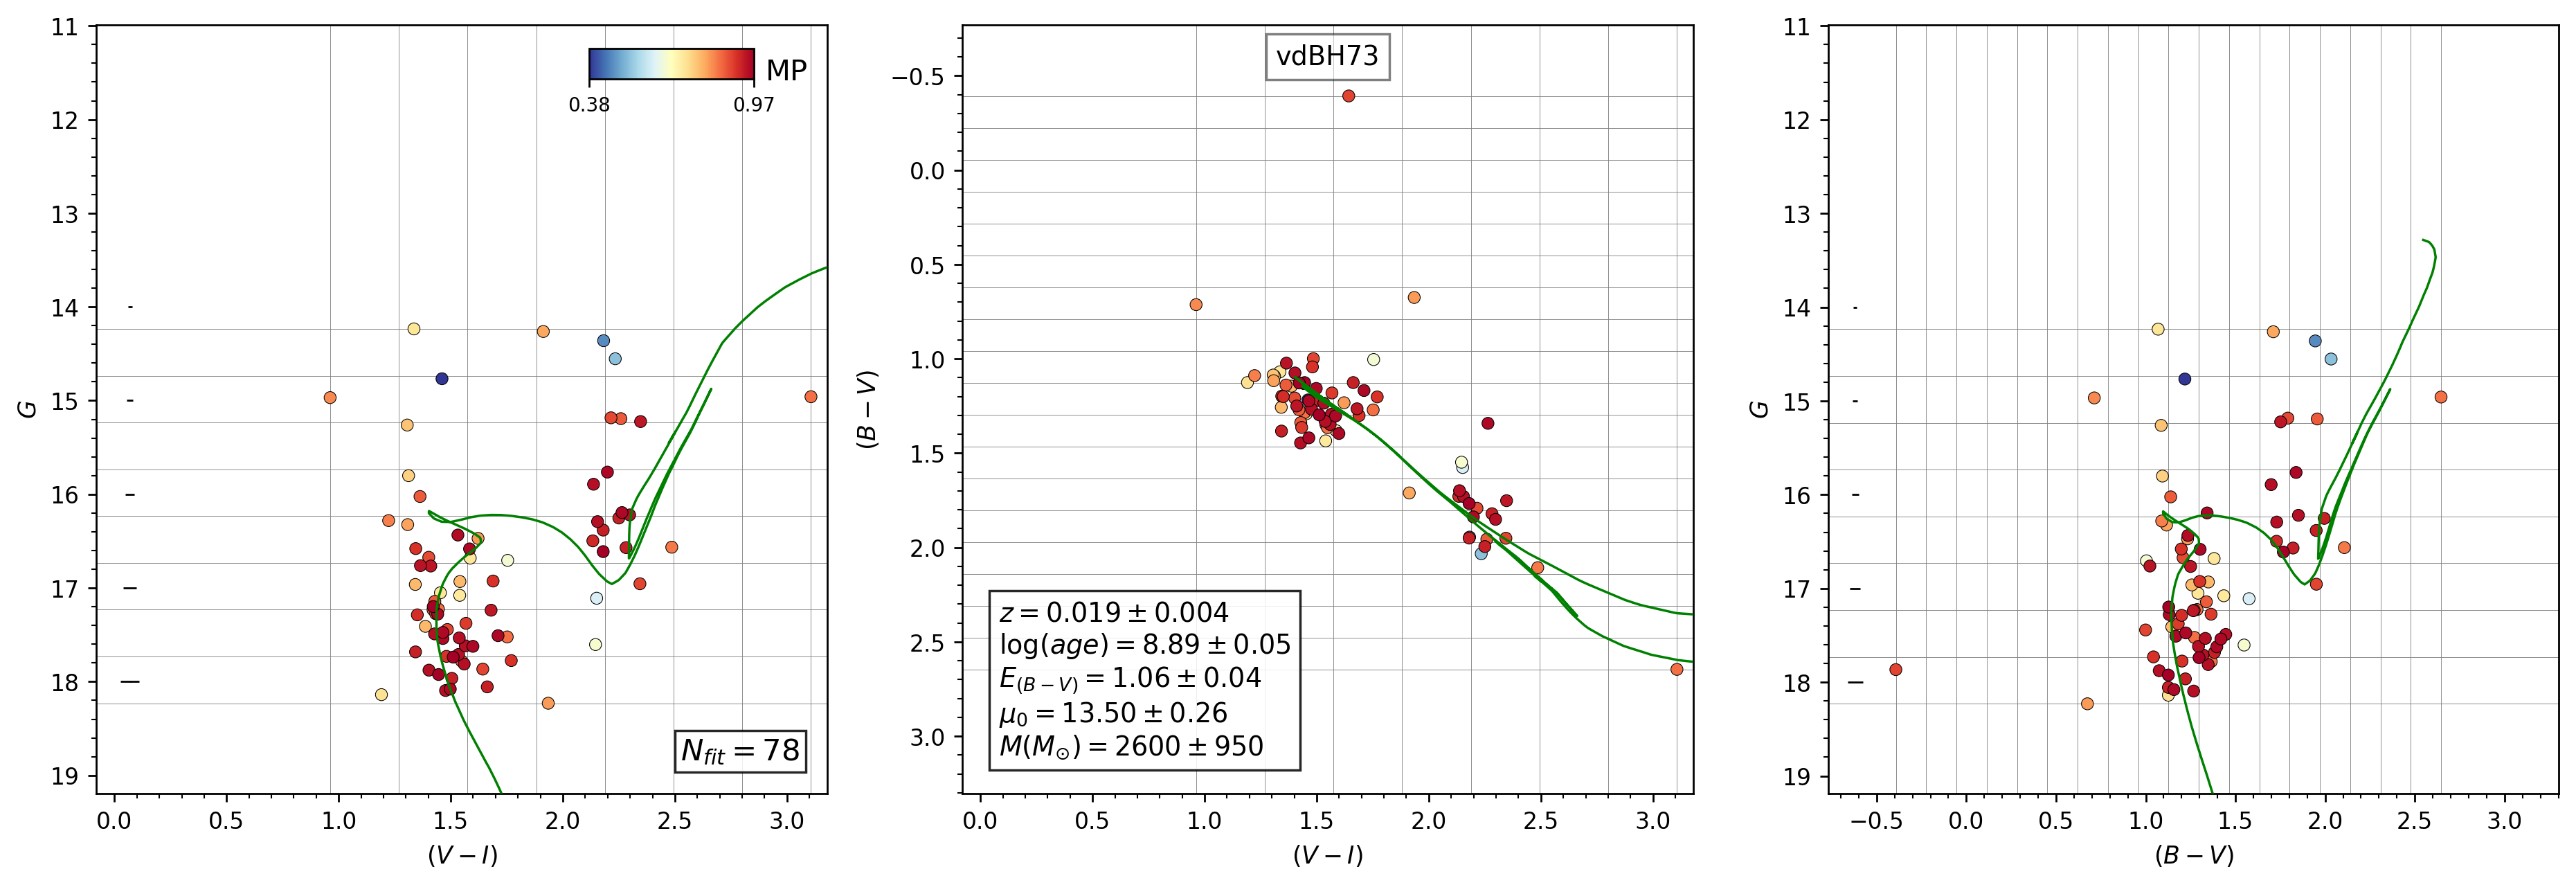
\includegraphics[width=\hsize]{../figs/cmds_vdBH73.png}
\caption{Idem Fig. \ref{fig:fundpars_vdBH85} for vdBH 73 with the $(B-V)$ vs
$(V-I)$ diagram instead of the $(B-V)$ vs $(U-B)$ diagram.}
    \label{fig:fundpars_vdBH73}
\end{figure*}

\begin{figure*}[ht]
    \centering
    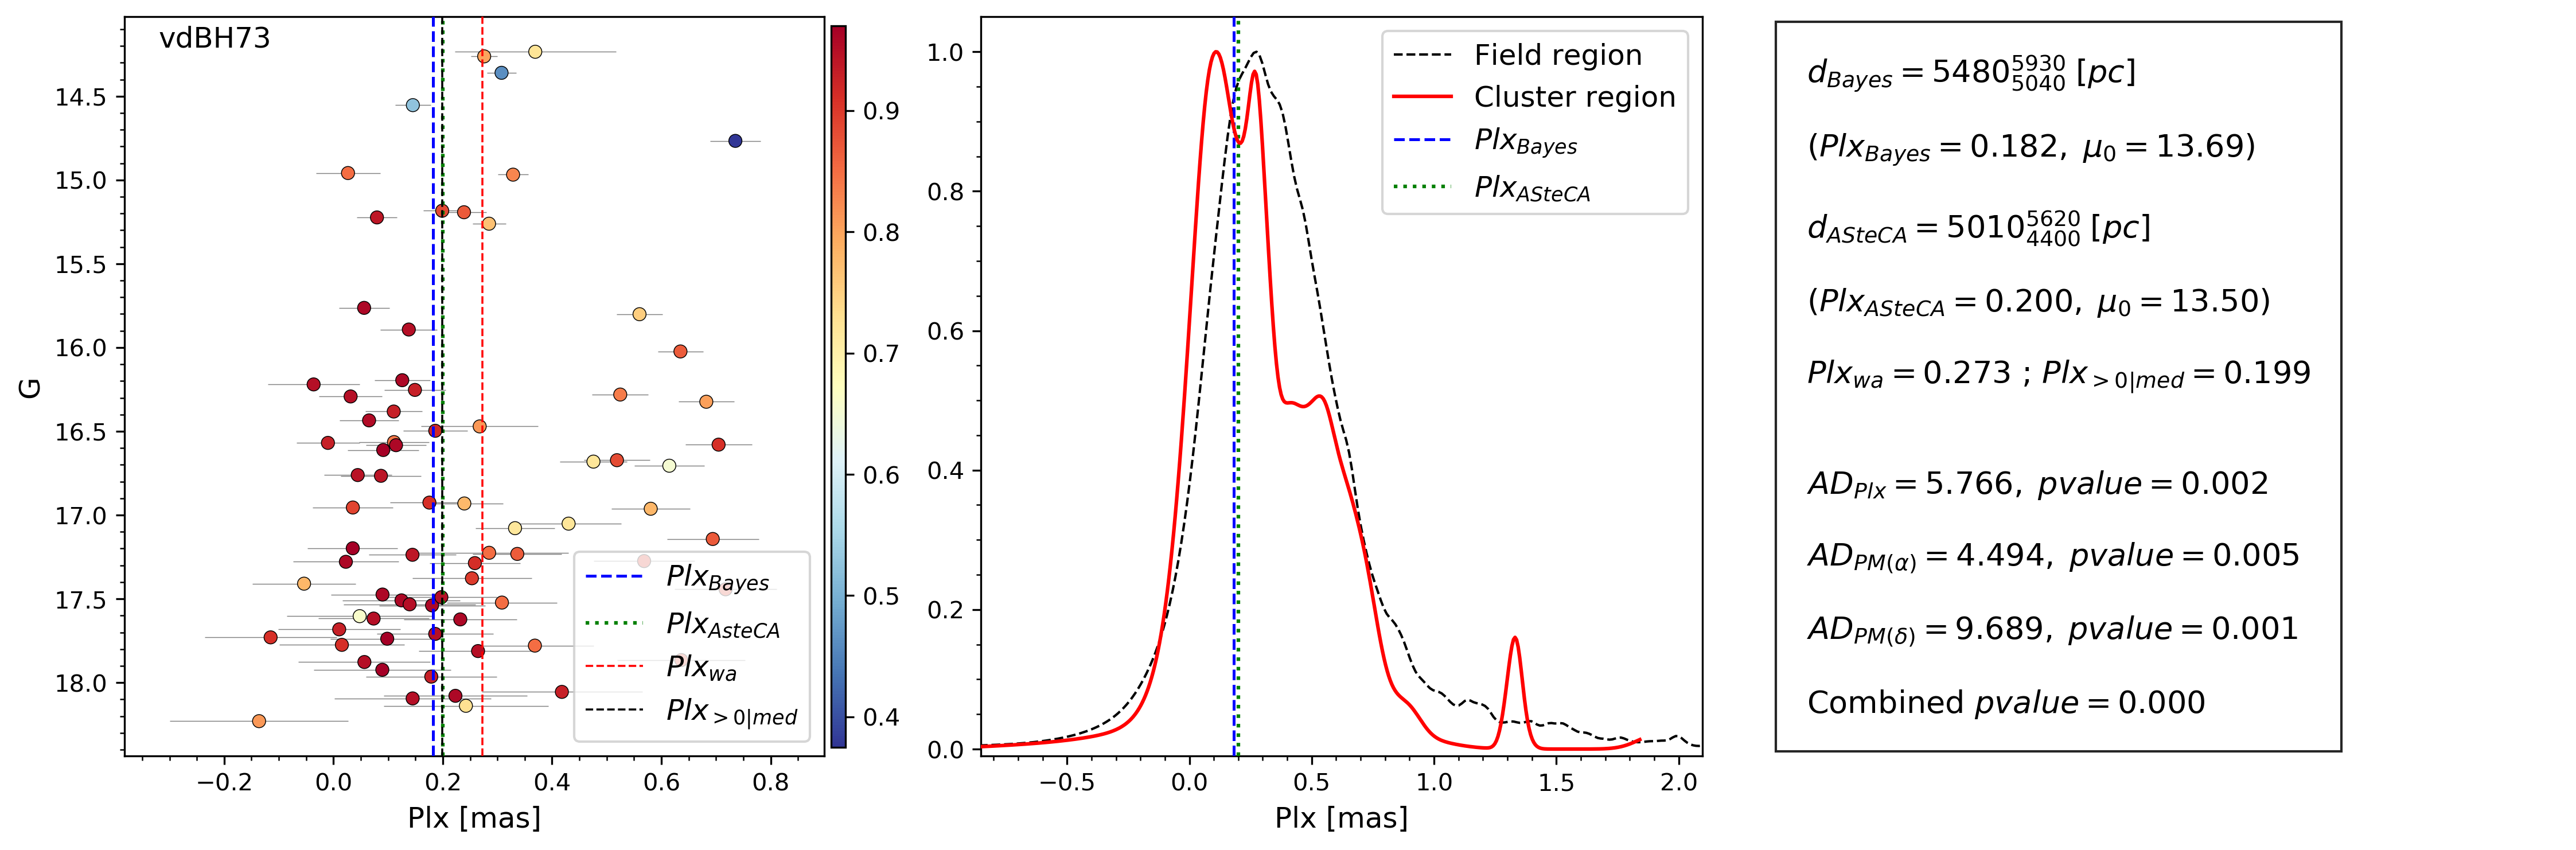
\includegraphics[width=\hsize]{../figs/plx_vdBH73.png}
\caption{Idem Fig. \ref{fig:plx_bys_vdBH85} for vdBH 73.}
\label{fig:plx_bys_vdBH73}
\end{figure*}




%================================================================
\section{Ruprecht 85}

Ruprecht 85 belongs to the south side of the Vela constellation close to the
border of the Carina region. This cluster appears in Fig. \ref{fig:Vim} as a
slight increment in the stellar field toward the north part in the respective
frame.
The overall stellar photometric diagrams as shown in Fig. \ref{fig7} do not show any cluster sequence, but a vertical strip of stars emerging from
a poorly populated stellar field above $G=14$ mag defined by disk stars.\\

The structural analysis performed by \texttt{ASteCA} yields a clean overdensity
at the location of this object that appears to subtend an almost circular area
with a radius between 2-3 arcmin; see the left panel of Fig.~\ref{fig8}.
As shown in the right panel of Fig.~\ref{fig8}, the RDP is well developed
and with a stellar density five times above the background level. The
photometric diagrams, CCD and CMDs of stars with membership probabilities above
0.48 and up to 1.0 shown in Fig. \ref{fig9} depict a rather noisy main
sequence sweeping 3.5 magnitudes.
Combining structural evidences with evidences coming from the photometric
diagrams we conclude that RUP 85 is a real entity. As for the cluster
parameters of the best synthetic cluster fitting the observations it is found
that:

\begin{itemize}
\item [a)] As is the case with vdBH 73, RUP 85 is also placed
in a region of moderate color excess. The cluster has $E(B-V)=1.06,$
also entirely in line with a maximum $E(B-V)$ of 2 mag according to S\&F2011.
\item [b)] The free absorption distance modulus is $13.40\pm0.12$ mag,
corresponding to a distance $d=4.80\pm0.26$ kpc.
\end{itemize}

The results from the Anderson-Darling test in Fig. \ref{fig10} applied to $Plx$,
$PM(\alpha),$ and $PM(\delta)$ clearly indicate that the cluster region and the
surrounding background population come from quite different stellar populations.
Therefore the null hypothesis can be rejected.\\

We conclude that RUP 85 is a real open cluster that is about $0.18\pm0.03\times10^9$
years old.

\begin{figure*}[ht]
    \centering
    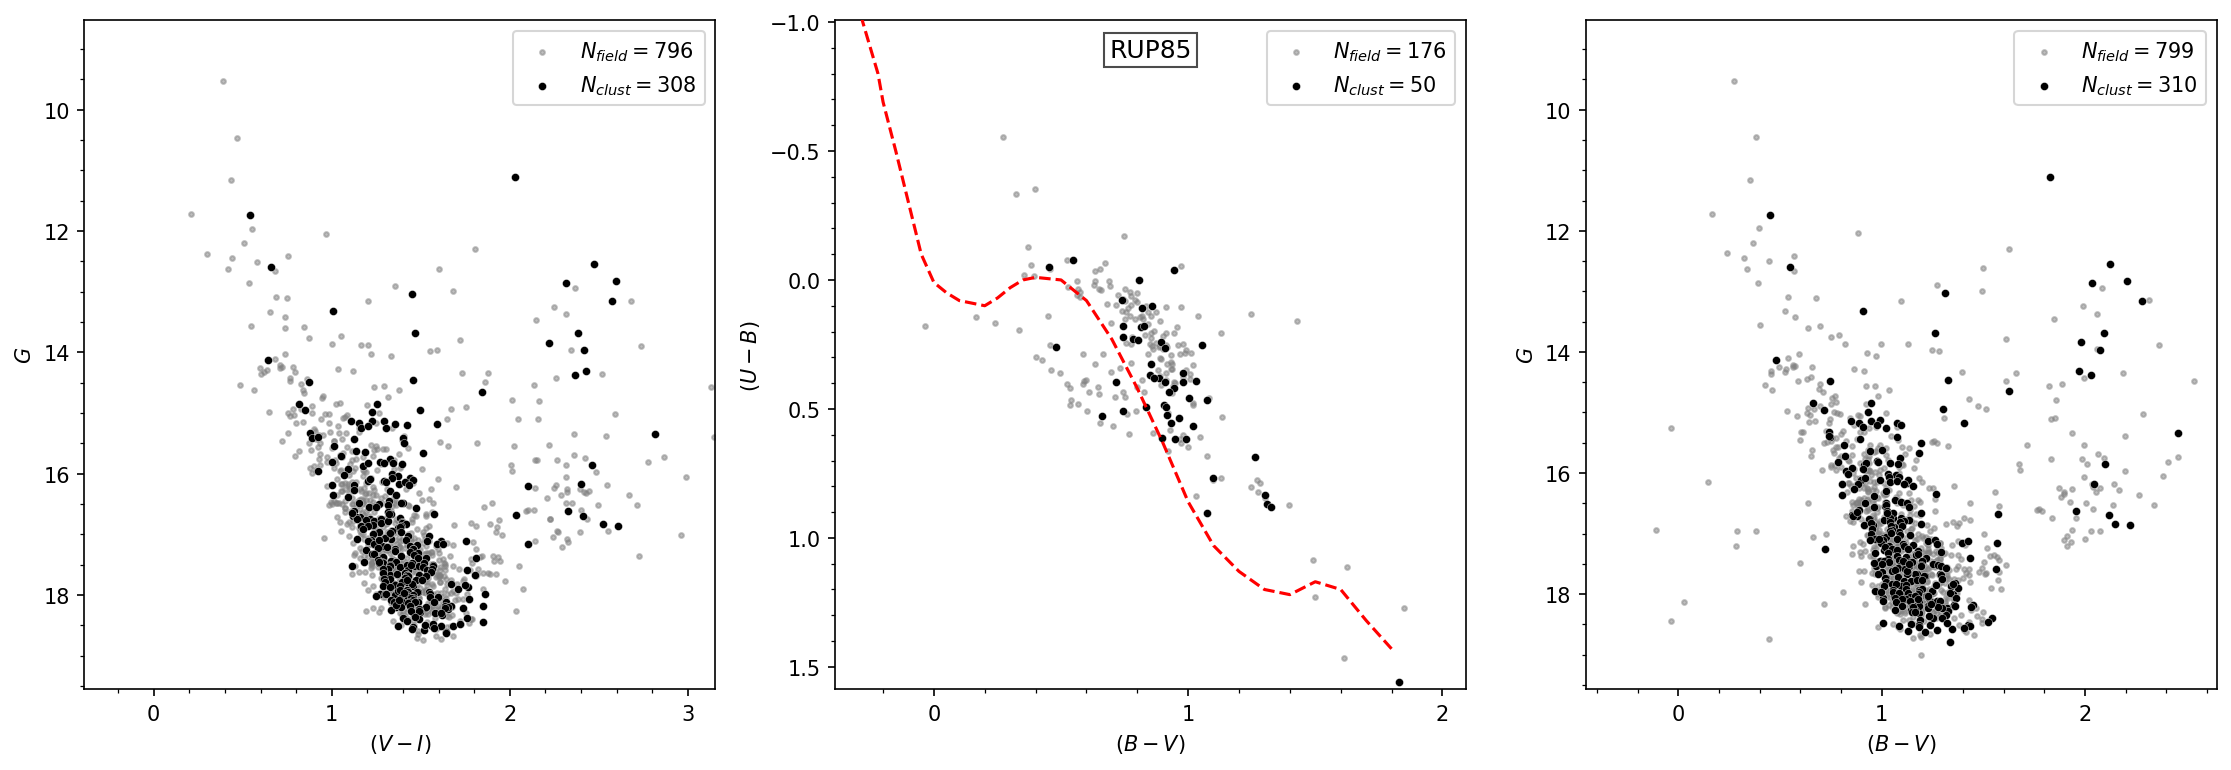
\includegraphics[width=\hsize]{../figs/obs_RUP85.png}
    \caption{Idem Fig. \ref{fig:photom_vdBH85} for RUP 85.}
    \label{fig7}
\end{figure*}

\begin{figure*}[ht]
    \centering
    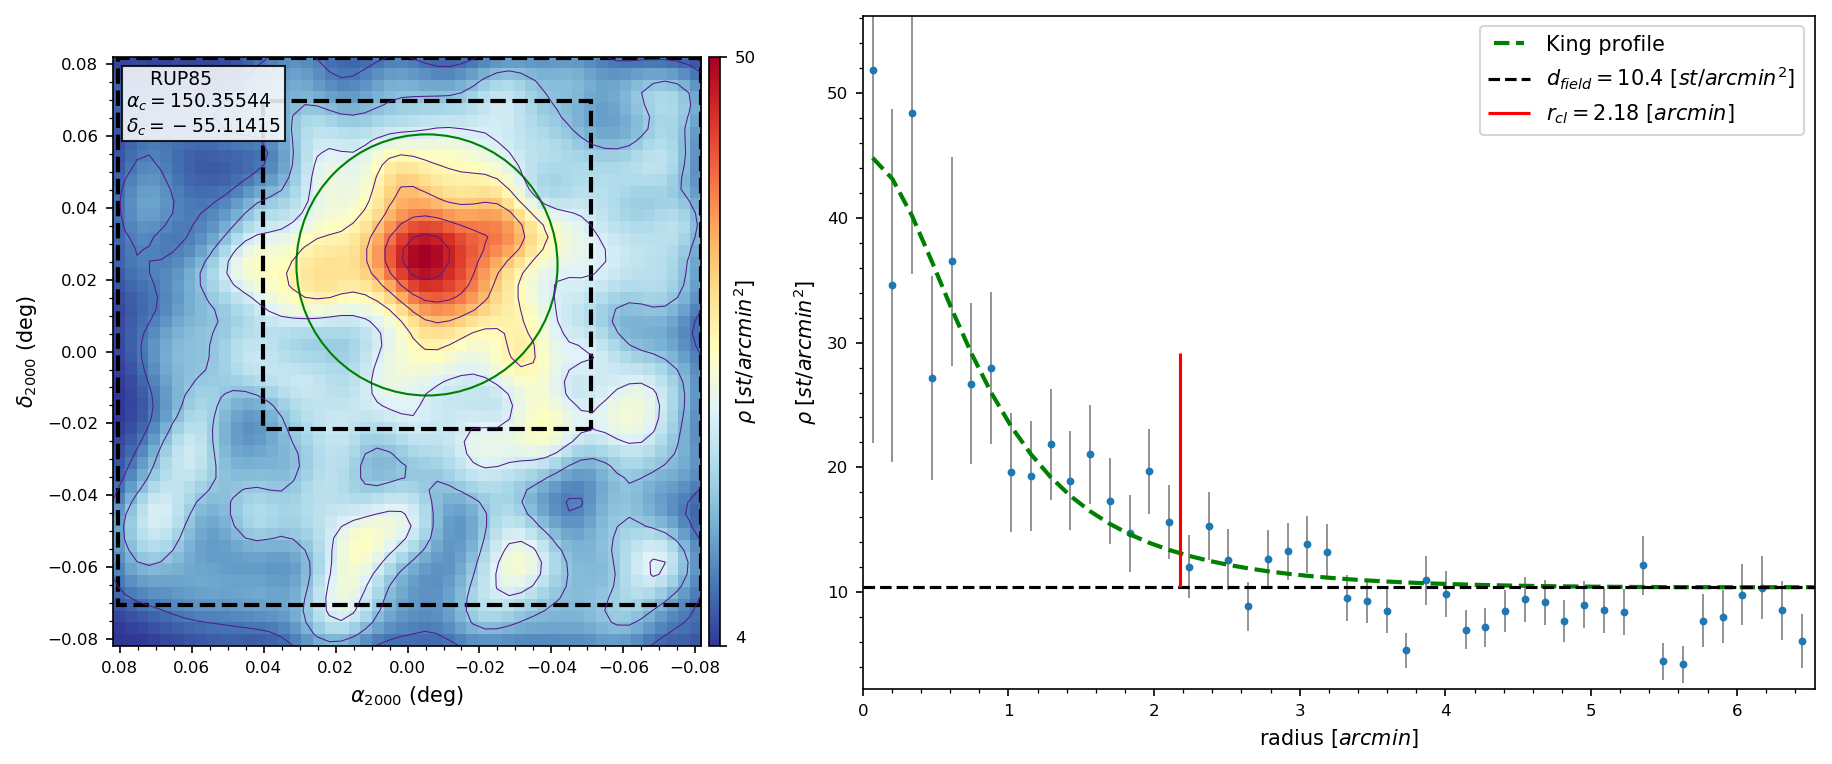
\includegraphics[width=\hsize]{../figs/dmap_rup85.png}
    \caption{Idem Fig. \ref{fig:struct_vdBH85} for RUP 85.}
    \label{fig8}
\end{figure*}

\begin{figure*}[ht]
    \centering
    \includegraphics[width=\hsize]{../figs/cmds_rup85.png}
    \caption{Idem Fig. \ref{fig:fundpars_vdBH85} for RUP 85.}
    \label{fig9}
\end{figure*}

\begin{figure*}[ht]
    \centering
    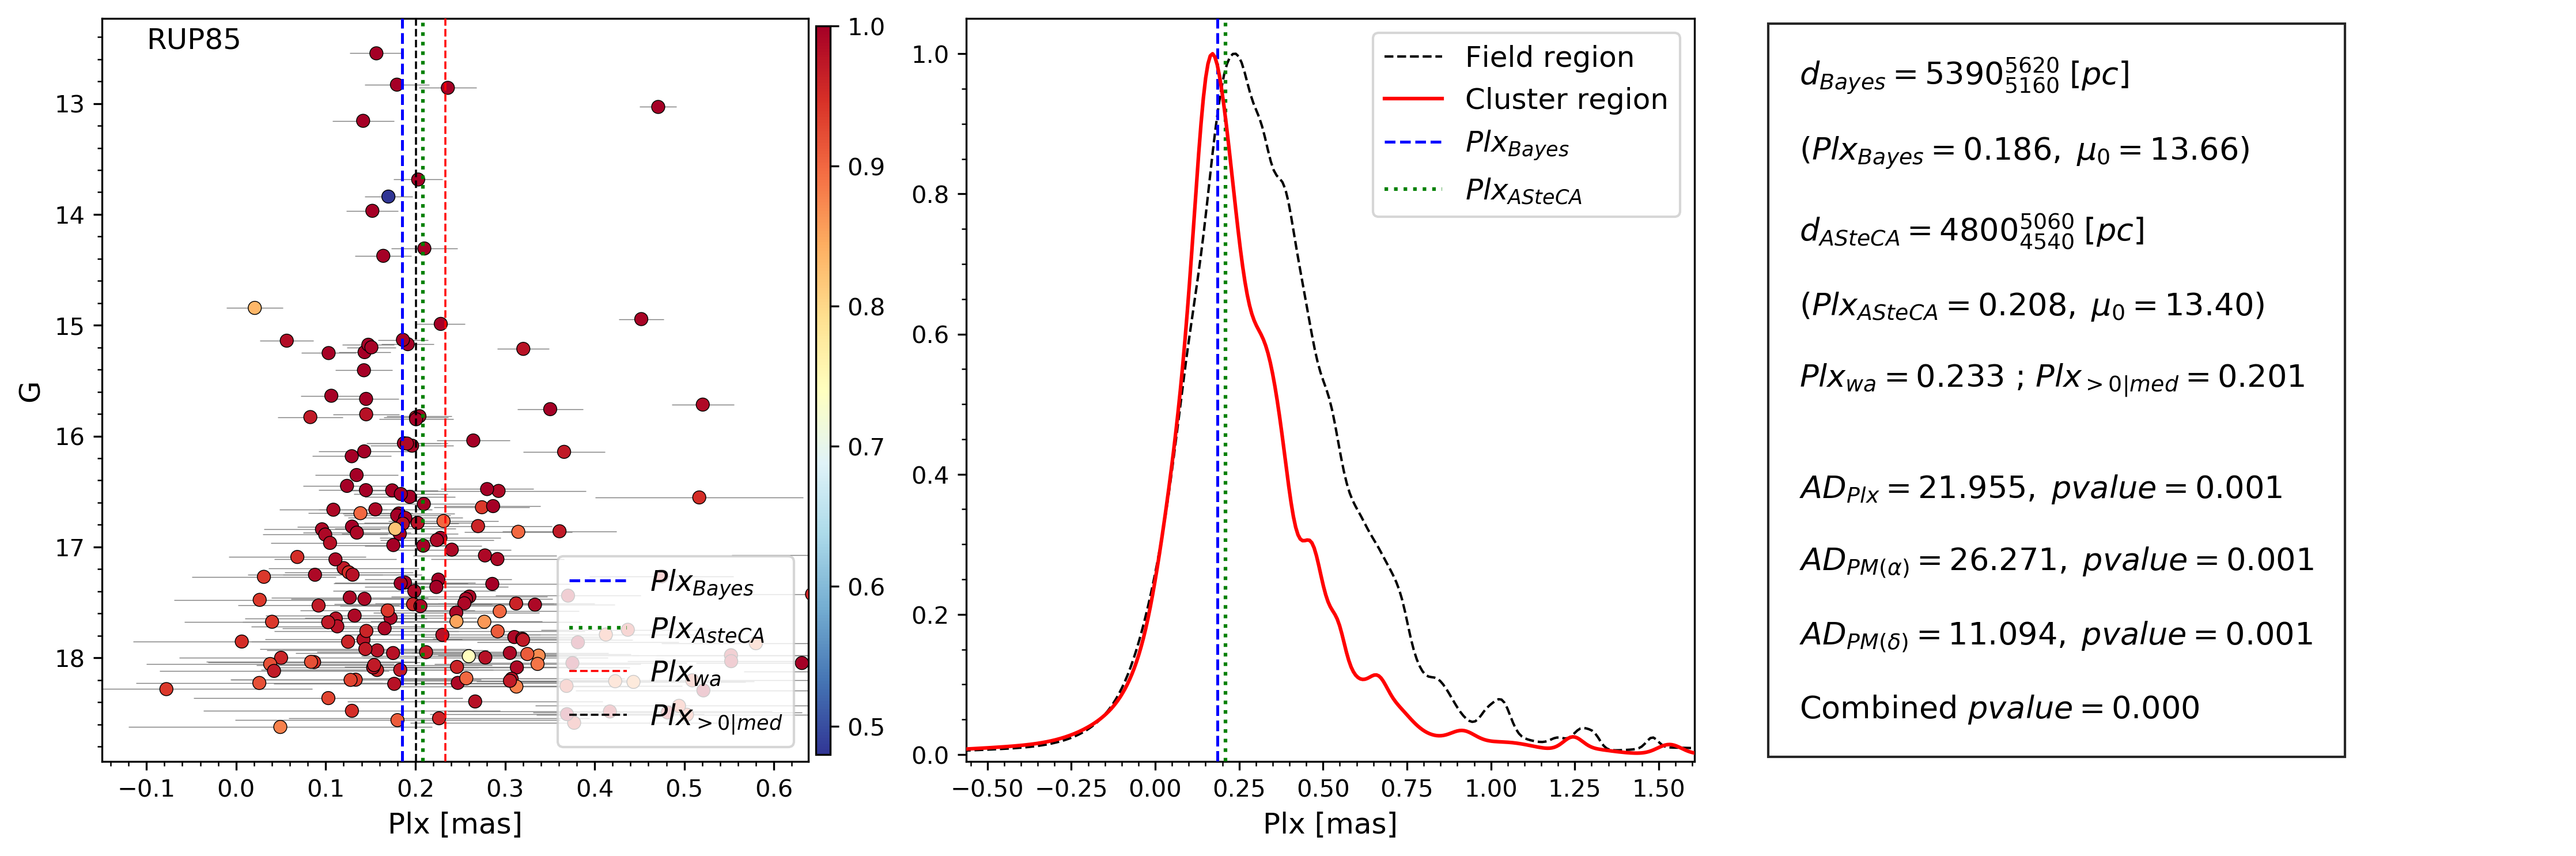
\includegraphics[width=\hsize]{../figs/plx_RUP85.png}
    \caption{Idem Fig. \ref{fig:plx_bys_vdBH85} for RUP 85.}
    \label{fig10}
\end{figure*}





%================================================================
\section{van den Bergh-Hagen 87}

Like RUP 85, vdBH 87 is seen toward the south of the Vela constellation close to
the border with Carina. A weak grouping of stars placed toward the north of
the frame is shown in Fig. \ref{fig:Vim}. In turn, the CMDs in Fig. \ref{fig15}
seem to reflect a typical stellar disk sequence up to approximately $G=15$ mag,
with an amorphous distribution at the bright end. The CCD, on the other
hand, is rather poor.\\

A stellar overdensity reaching $\text{about seven}$ times the field stellar density is
shown in Fig. \ref{fig16}. The spatial structure of this overdensity suggests an
elongation in right ascension and an RDP characterized by a very narrow density
peak followed by a stellar coronal distribution at about 1.5 arcmin from the
center.
The clean CMDs in Fig. \ref{fig17} clearly show the nature of vdBH 87
because inside this overdensity, a clear and narrow cluster main
sequence is evident. Its sequence extends for more than 5 mag in the
CMDs, including stars with very low membership probabilities well detached
from the sequence, in the range from 0.0 to 0.98. The parameters of the
synthetic cluster that best fits the real stellar distributions are listed below.

\begin{itemize}
\item [a)] The color excess is $E(B-V)=0.56,$ indicating thus a moderate
    absorption in the cluster direction. This color excess value in turn is
    below the maximum reddening $E(B-V)=2.9$ computed in the region by 
    S\&F2011.
\item [b)] The corrected distance modulus is $11.59\pm0.09$ mag, implying a
distance of $d=2.08\pm0.09$ kpc. The cluster is not far from the Sun, and
this closeness explains the moderate color excess we found.
\end{itemize}

The results of applying the Anderson-Darling test in Fig. \ref{fig18}
are coincident with what \texttt{ASteCA}  found: cluster and
field regions are quite different not only from the photometric perspective, but
also from a kinematic view.
In conclusion, vdBH 87 is a real open cluster that is $0.25\pm0.08\times10^9$
years old.

\begin{figure*}[ht]
    \centering
    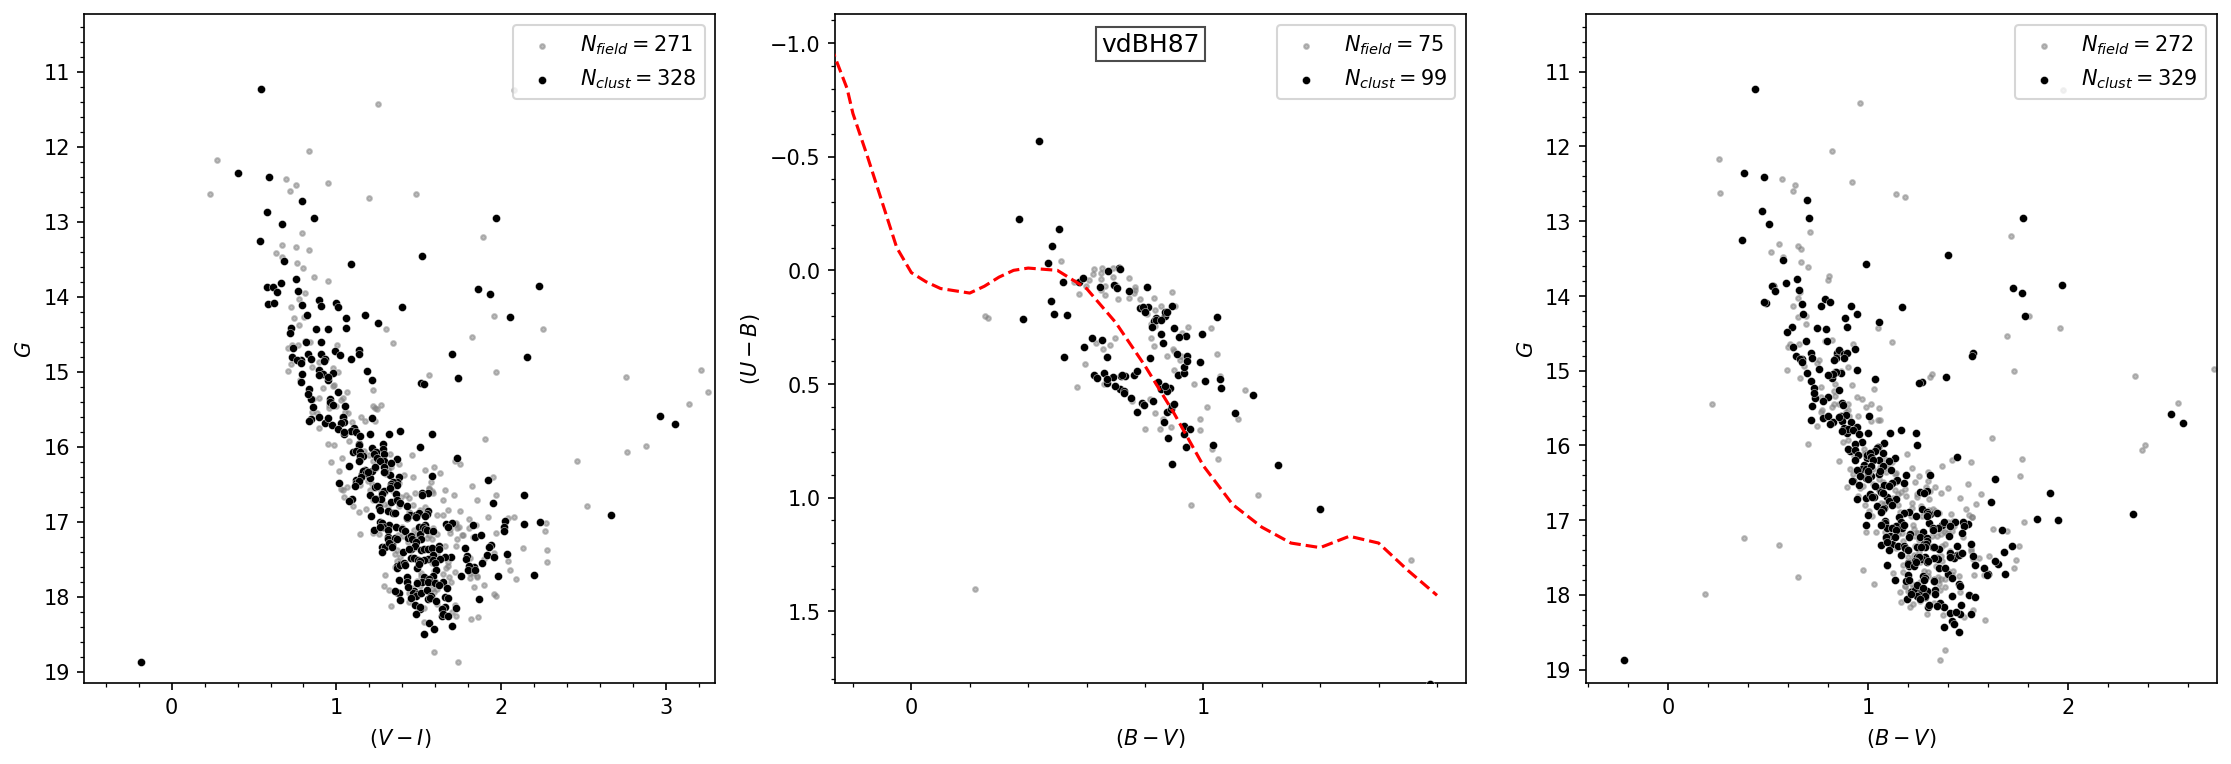
\includegraphics[width=\hsize]{../figs/obs_vdBH87.png}
    \caption{Idem Fig. \ref{fig:photom_vdBH85} for vdBH 87.}
    \label{fig15}
\end{figure*}

\begin{figure*}[ht]
    \centering
    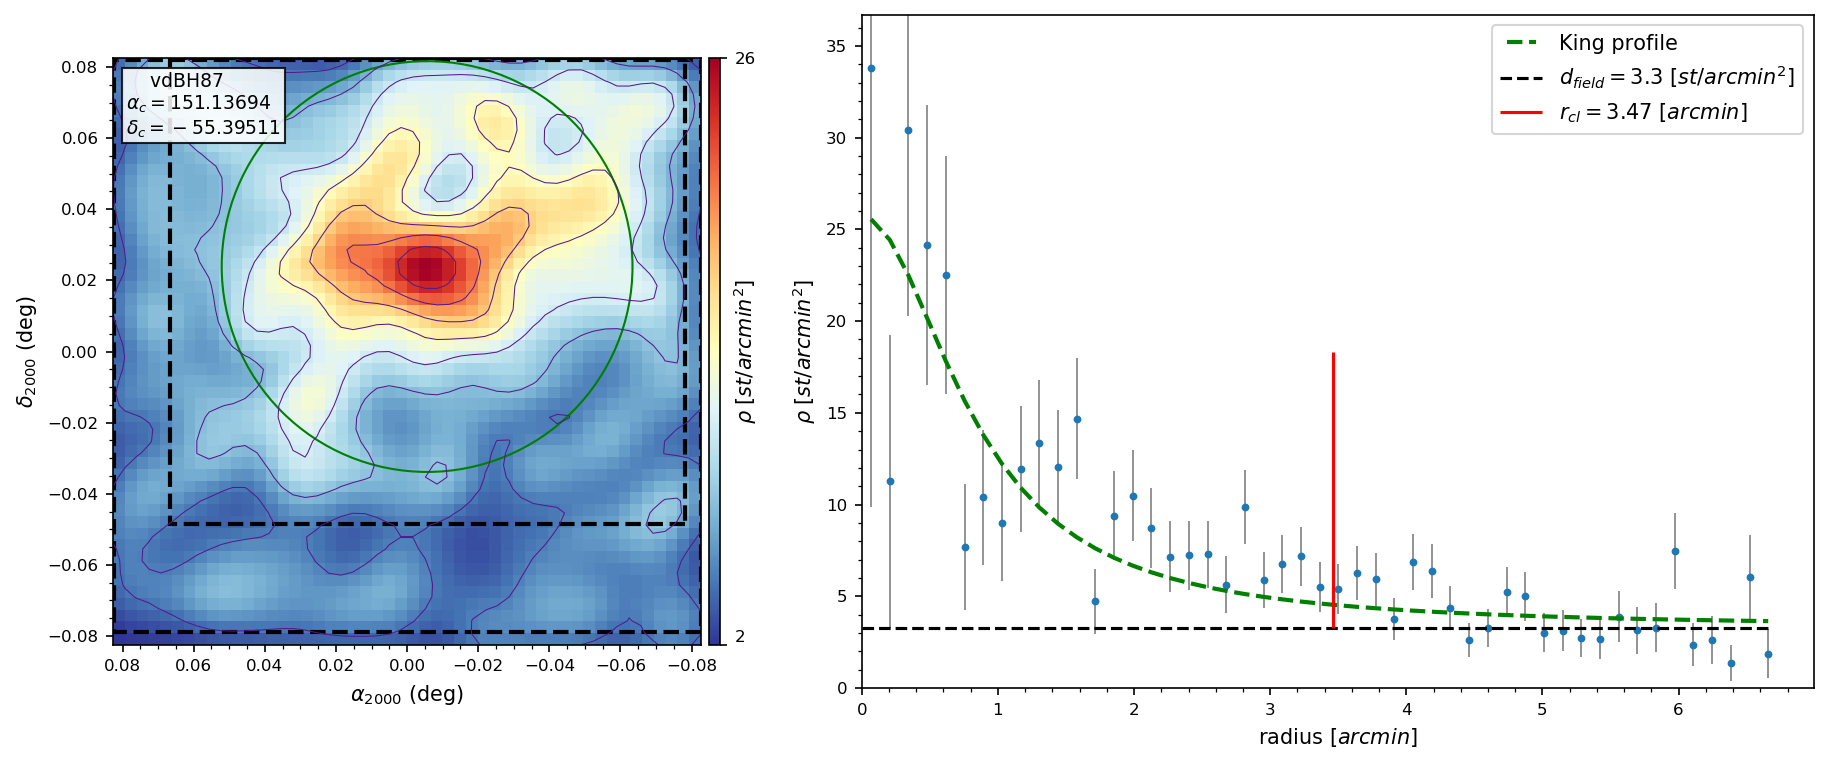
\includegraphics[width=\hsize]{../figs/dmap_vdbh87.png}
    \caption{Idem Fig. \ref{fig:struct_vdBH85} for vdBH 87.}
    \label{fig16}
\end{figure*}

\begin{figure*}[ht]
    \centering
    \includegraphics[width=\hsize]{../figs/cmds_vdbh87.png}
    \caption{Idem Fig. \ref{fig:fundpars_vdBH85} for vdBH 87.}
    \label{fig17}
\end{figure*}
\begin{figure*}[ht]
    \centering
    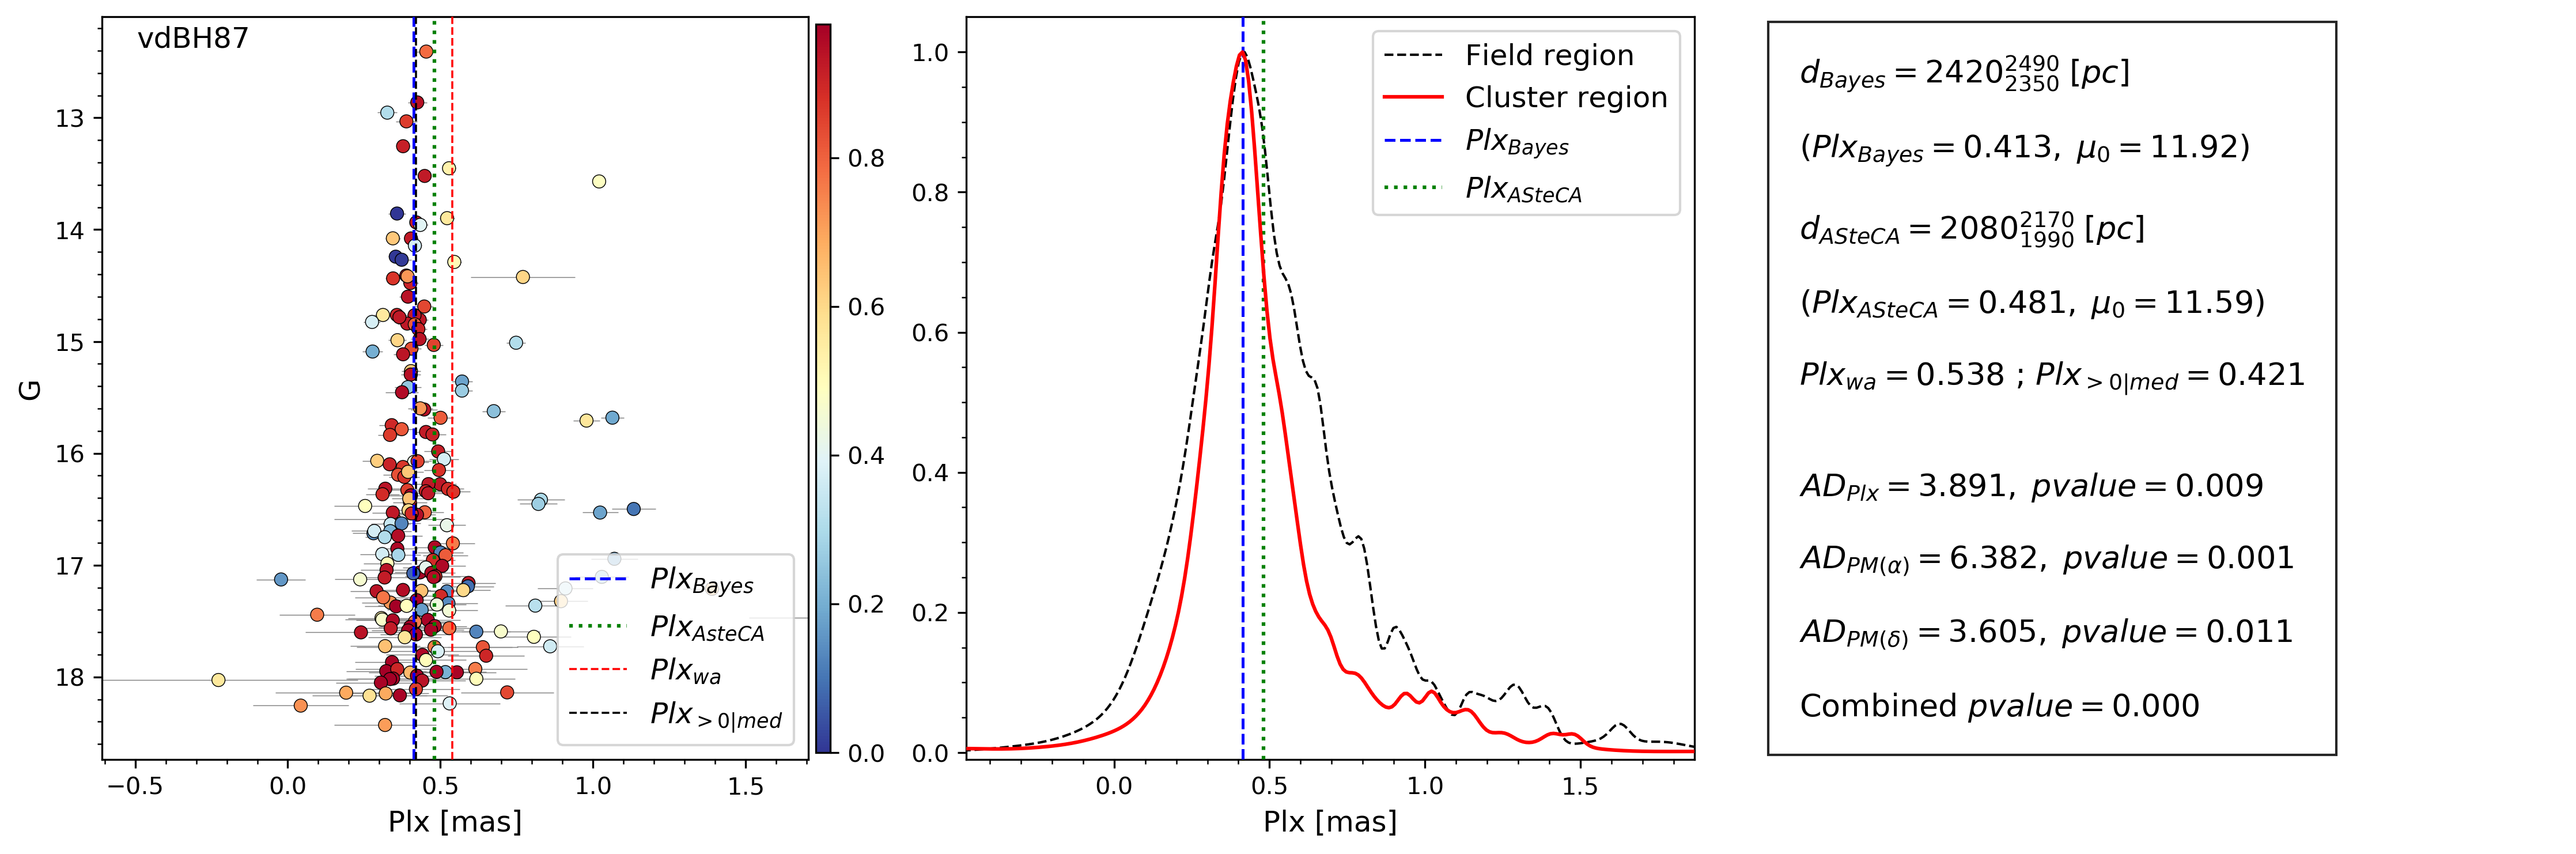
\includegraphics[width=\hsize]{../figs/plx_vdBH87.png}
    \caption{Idem Fig. \ref{fig:plx_bys_vdBH85} for vdBH 87.}
    \label{fig18}
\end{figure*}




%================================================================
\section{van den Bergh-Hagen 92}

Placed south of Vela, near the eastern border with Carina, vdBH
92 is a relevant handful of bright stars as shown in the $V$ image of Fig.
\ref{fig:Vim}. The CMDs and CCD for all stars in the region, as shown in Fig.
\ref{fig35}, depict a narrow stellar sequence with some scatter at their respective
bright ends. Particularly the CCD shows a
group of $F$- and $G$-type stars close to the intrinsic line, and another group of stars below the intrinsic
line that might be $B$- and $A$-type stars displaced by the reddening effect.\\

The \texttt{ASteCA} analysis in Fig. \ref{fig36} revealed a
well-isolated stellar overdensity that rose above the field stellar density of
about six stars per square arcminute. We identify this overdensity with vdBH
92. \textbf{Notwithstanding} the noisy RDP, the limits of the overdensity can
still be well established. As indicated in Fig. \ref{fig37}, only a few stars
have been found inside the cluster limits, mostly with high membership values.
Despite the low number of members, a cluster main sequence extended by seven
magnitudes is visible. The comparison with synthetic clusters made by 
\texttt{ASteCA} yields that

\begin{itemize}
\item [a)] the best-fit of a synthetic cluster to the clean data in Fig. 
    \ref{fig37} indicates a color excess of $E(B-V)=0.65$. Because the
    maximum color excess provided by S\&F2011 is 2.34 for this zone, we
    conclude that most of the absorption is produced behind the position of
    vdBH 92. This object is therefore placed in front of a strong
    absorption region.
\item [b)] the absorption-free distance modulus becomes
$12.07\pm0.09$ mag, which places vdBH 92 at a distance of $d=2.59\pm0.11$ kpc.
\end{itemize}

By applying the Anderson-Darling test, we note that the parallax
distributions for stars inside and outside the cluster boundaries are not
sufficiently different from each other to reach the 5\% critical value, as
indicated in the right panel of Fig. \ref{fig38}. However, proper motions are
quite different in both regions. We combine this last finding with the well-defined overdensity, which in turn shows a reasonable and
extended cluster main sequence, and conclude that the two samples come from
different populations.\\

These results together confirm the true nature of vdBH 92. This
young cluster is $0.02\pm0.01\times10^9$ years old; it is the youngest true cluster
in our sample.

\begin{figure*}[ht]
    \centering
    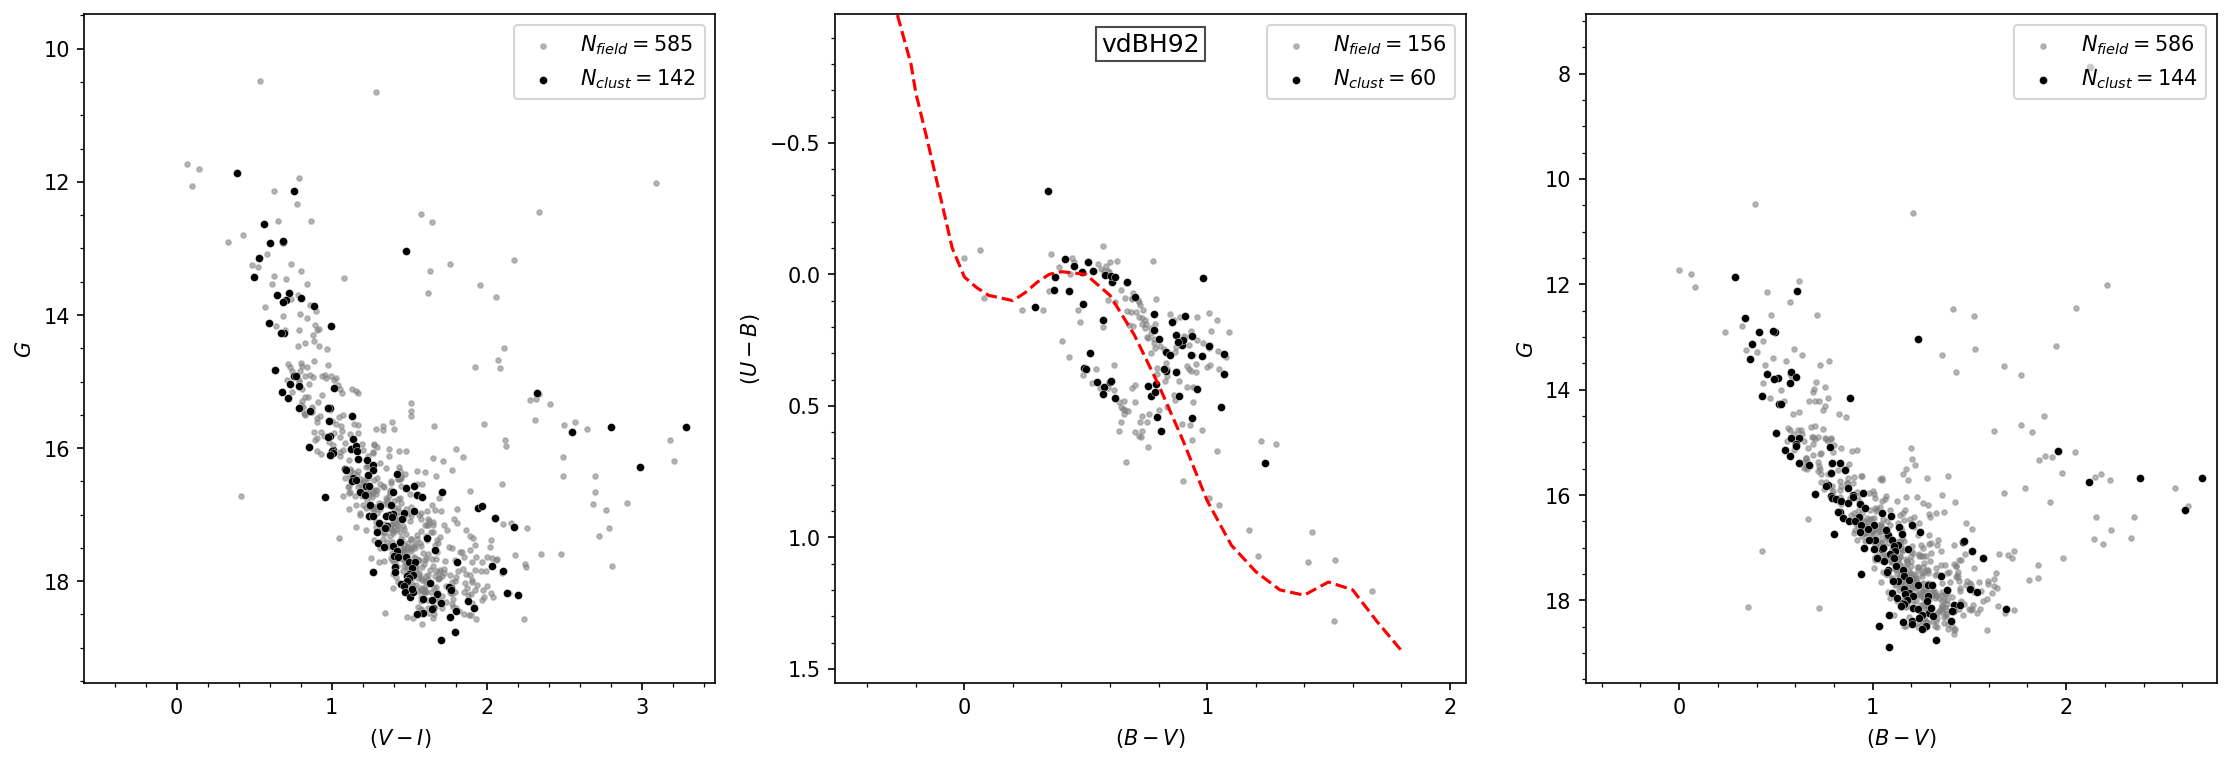
\includegraphics[width=\hsize]{../figs/obs_vdBH92.png}
    \caption{Idem Fig. \ref{fig:photom_vdBH85} for vdBH 92.}
    \label{fig35}
\end{figure*}
\begin{figure*}[ht]
    \centering
    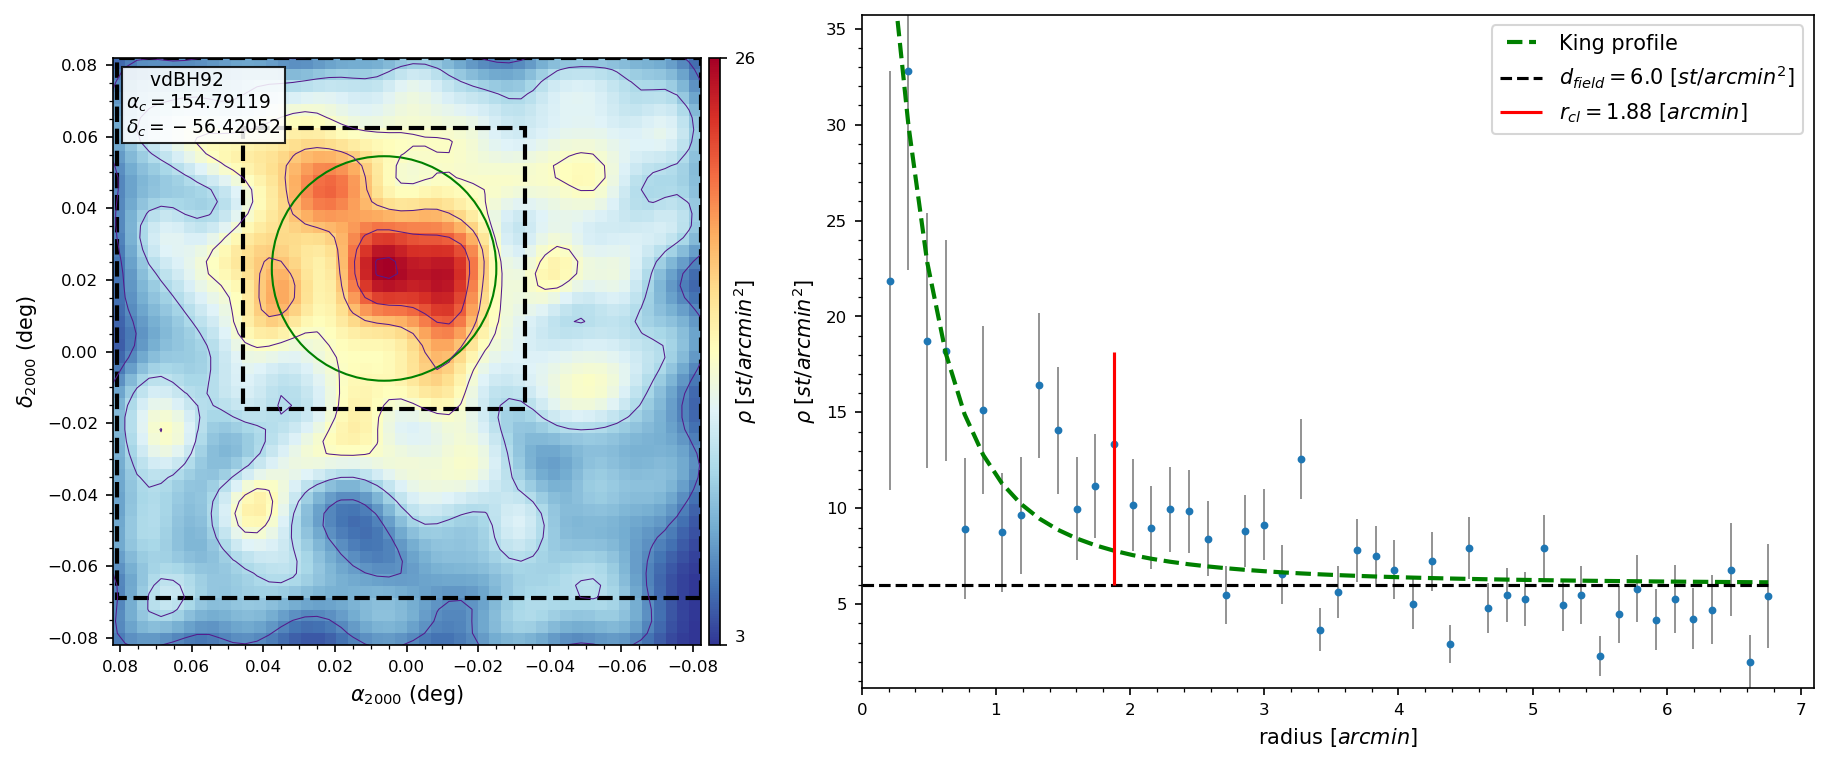
\includegraphics[width=\hsize]{../figs/dmap_vdbh92.png}
    \caption{Idem Fig. \ref{fig:struct_vdBH85} for vdBH 92.}
    \label{fig36}
\end{figure*}
\begin{figure*}[ht]
    \centering
    \includegraphics[width=\hsize]{../figs/cmds_vdbh92.png}
    \caption{Idem Fig. \ref{fig:fundpars_vdBH85} for vdBH 92.}
    \label{fig37}
\end{figure*}
\begin{figure*}[ht]
    \centering
    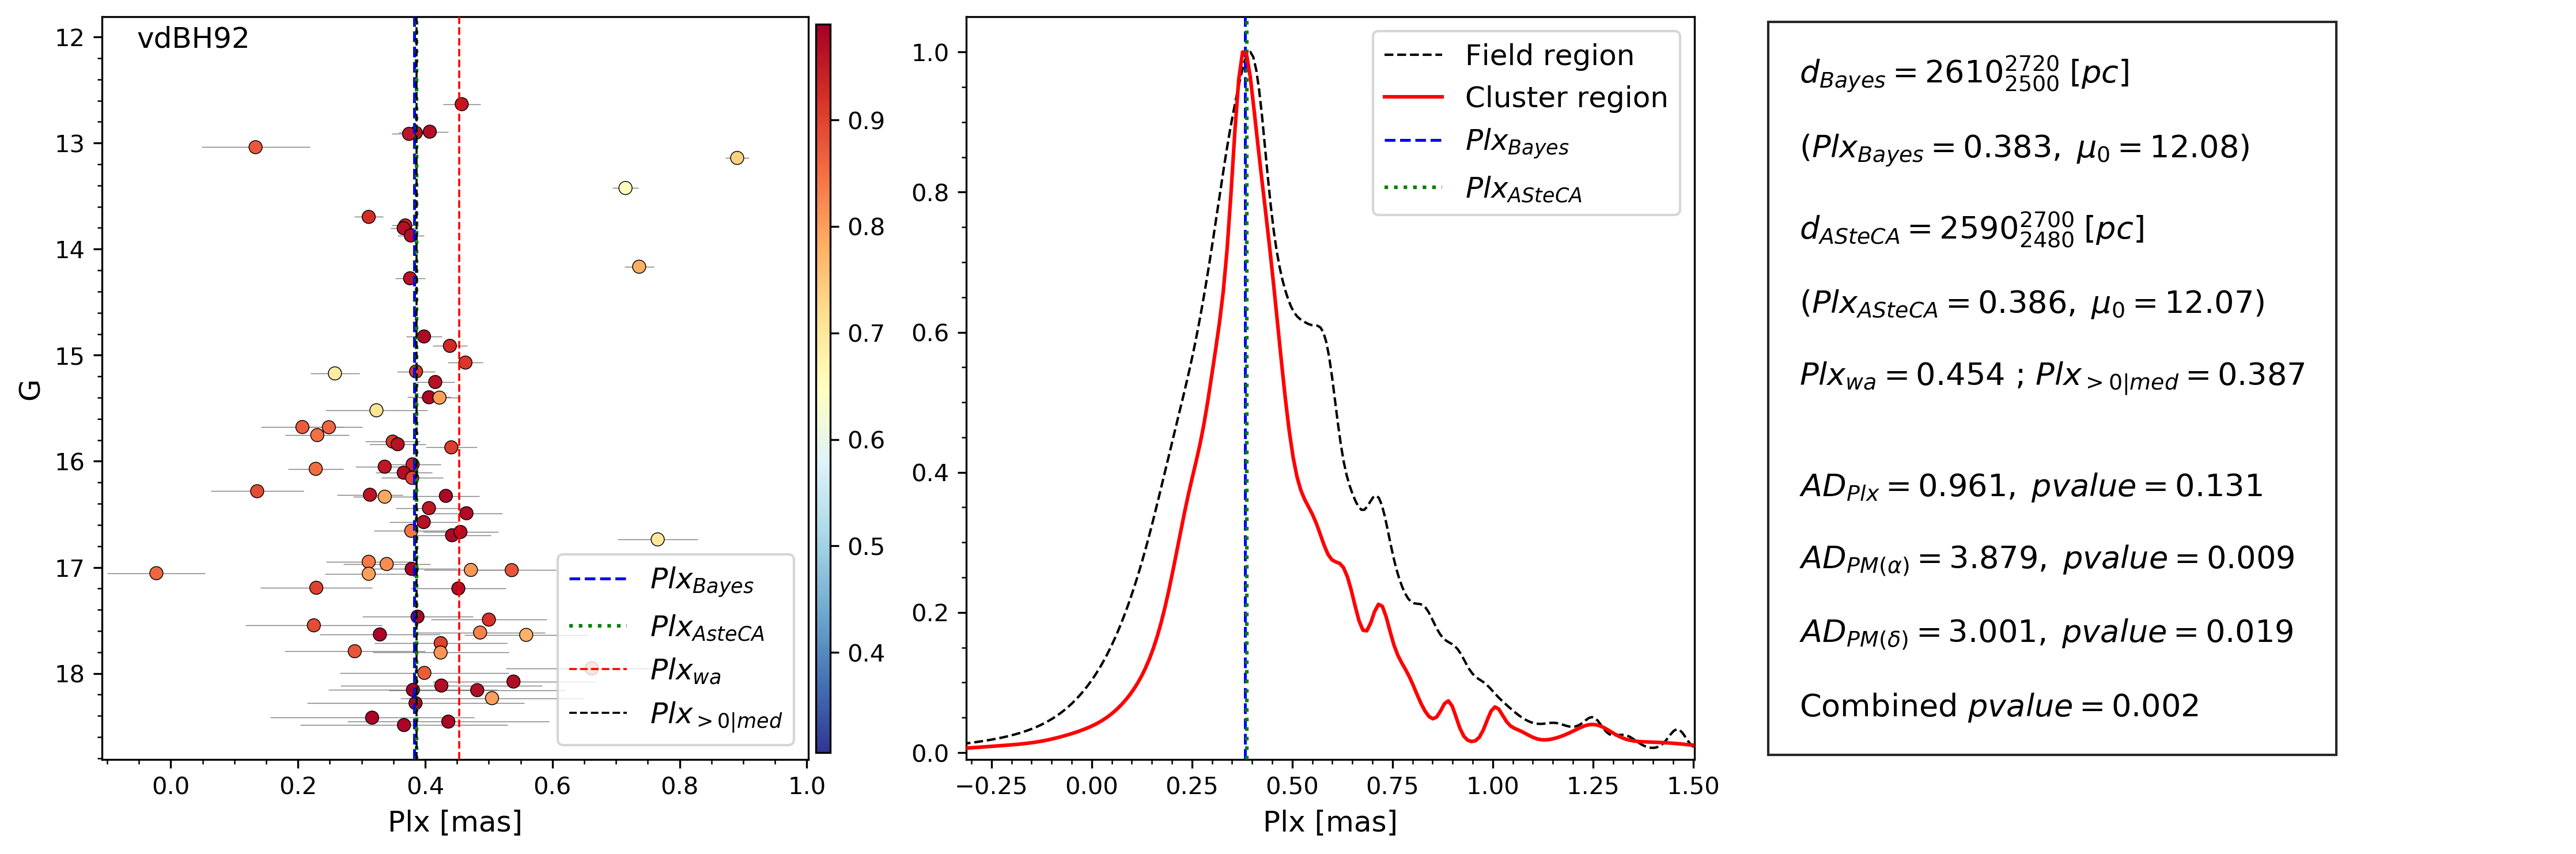
\includegraphics[width=\hsize]{../figs/plx_vdBH92.png}
    \caption{Idem Fig. \ref{fig:plx_bys_vdBH85} for vdBH 92.}
    \label{fig38}
\end{figure*}




%================================================================
\section{Trumpler 12}

This object is placed on the west side of the Carina HII region, where it appears
as a sparse handful of bright stars in Fig. \ref{fig:Vim}. The CMDs in Fig.
\ref{fig19}, including all stars in the region, show the following patterns:
there is a wide grouping of stars below $G=18$ mag, but to the right side of
it, and at this magnitude value, a narrow structure of stars up to $G=14$
mag is also slightly displaced to the blue side. From $G=18$ mag, a typical
vertical galactic disk population rises as well.\\

\texttt{ASteCA} detected a main overdensity in a region of high
stellar contamination, as shown in Fig.~\ref{fig20}.
This overdensity is characterized by a quite noisy RDP, which is partly
explained by the background density: at the peak of the RDP, this \textbf{is}
less than twice as high.
Under this condition, it is difficult to fix an appropriate
radius for the overdensity. We tentatively adopt a radius of $\sim2$ arcmin as a
reasonable compromise.
The membership probabilities in the zone of the overdensity are mostly
above 0.5, as indicated in Fig. \ref{fig21}. Again, as in vdBH 87, the
handful of stars with a low membership probability are very well detached from the main
cluster sequence.
%
A clear cluster main sequence is shown in Fig. \ref{fig21} to span about
4-5 mag. These stars belong to the tiny blue and narrow sequence that is
easily detected in the diagrams of Fig.~\ref{fig19} between $G=12$ and $G=16$
mag. Comparison with synthetic clusters yields the following values:

\begin{itemize}
\item [a)] A color excess of $E(B-V)=0.31$ is found for the best fit.
    Based on the maximum color excess provided by S\&F2011 of 0.50, we find that
    TR12 is placed in a zone of low absorption.
\item [b)] The absorption-free distance modulus is $12.7\pm0.09$ mag,
representing a distance of $3.50\pm0.15$ kpc. At this distance and with
low absorption, it is reasonable to find a high stellar background density,
as shown in Fig.~\ref{fig20}.
\end{itemize}

Based on the Anderson-Darling statistics shown in Fig.~\ref{fig21}, the
proper motions for the cluster and for the field population belong to different
samples. On the other hand, the parallaxes cannot be safely separated into
distinct stellar regions.\\

The clear cluster sequence and the low $p$-value (0.003) obtained with the AD
test lead us to conclude that TR 12 is a real cluster and is about
$0.70\pm0.10\times10^9$ years old.

\begin{figure*}[ht]
    \centering
    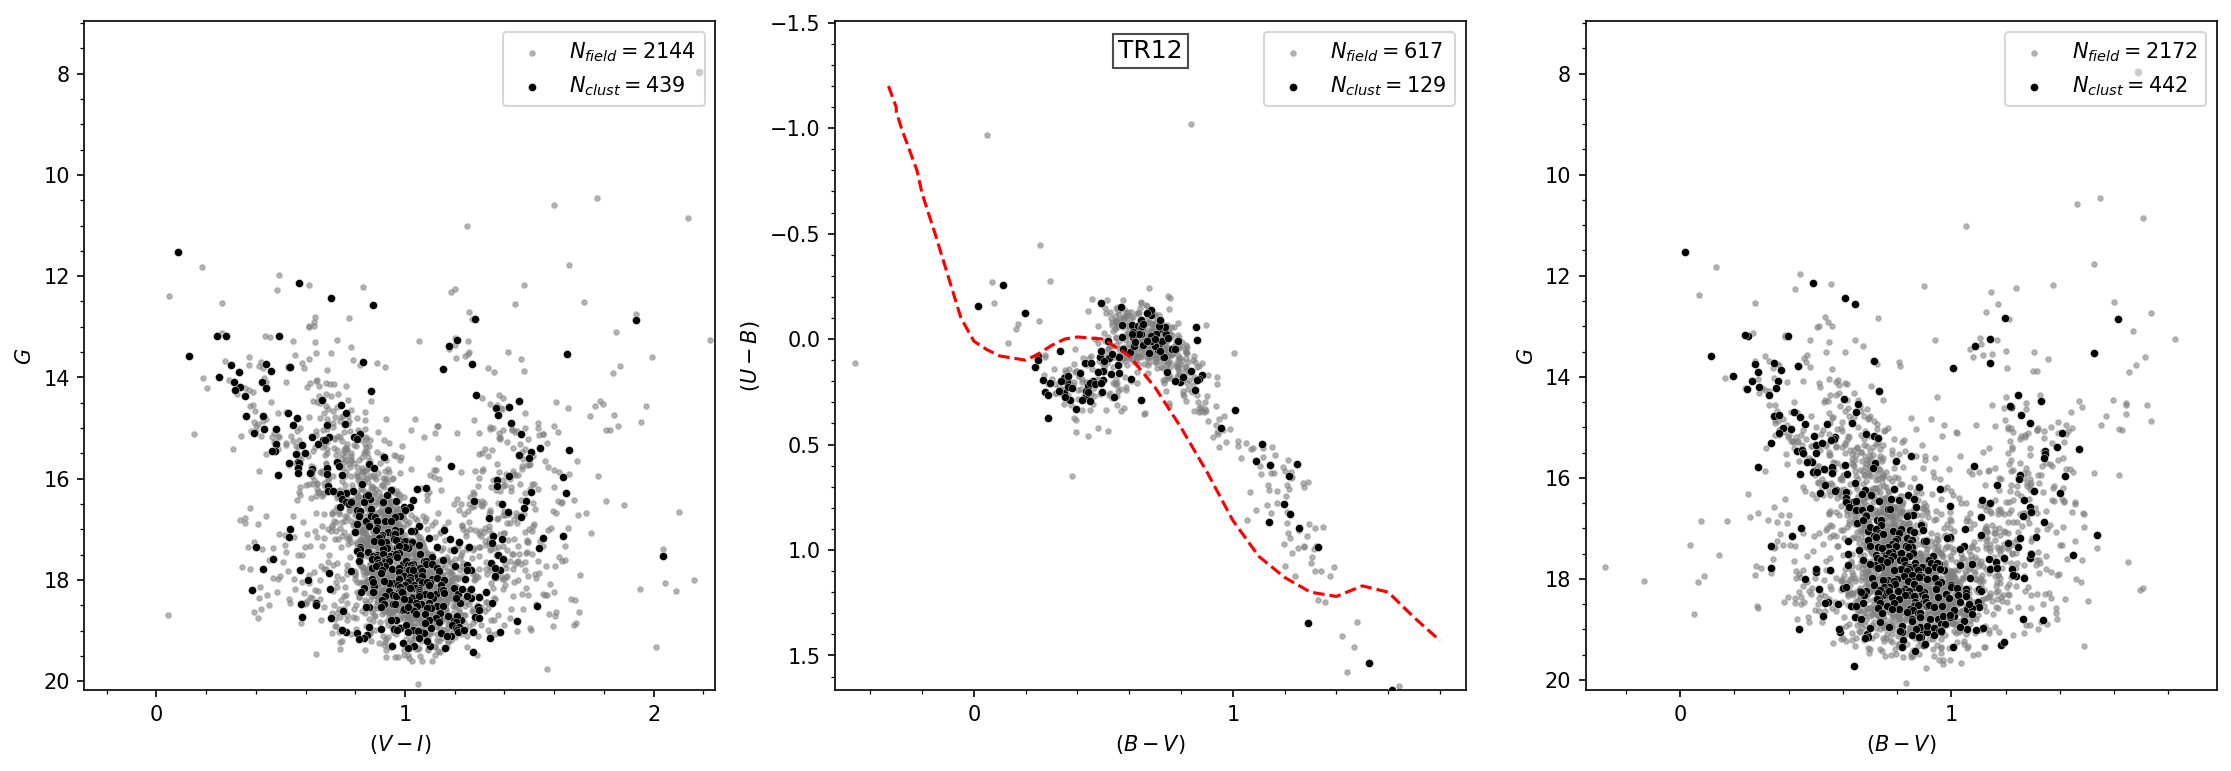
\includegraphics[width=\hsize]{../figs/obs_TR12.png}
    \caption{Idem Fig. \ref{fig:photom_vdBH85} for TR 12.}
    \label{fig19}
\end{figure*}
\begin{figure*}[ht]
    \centering
    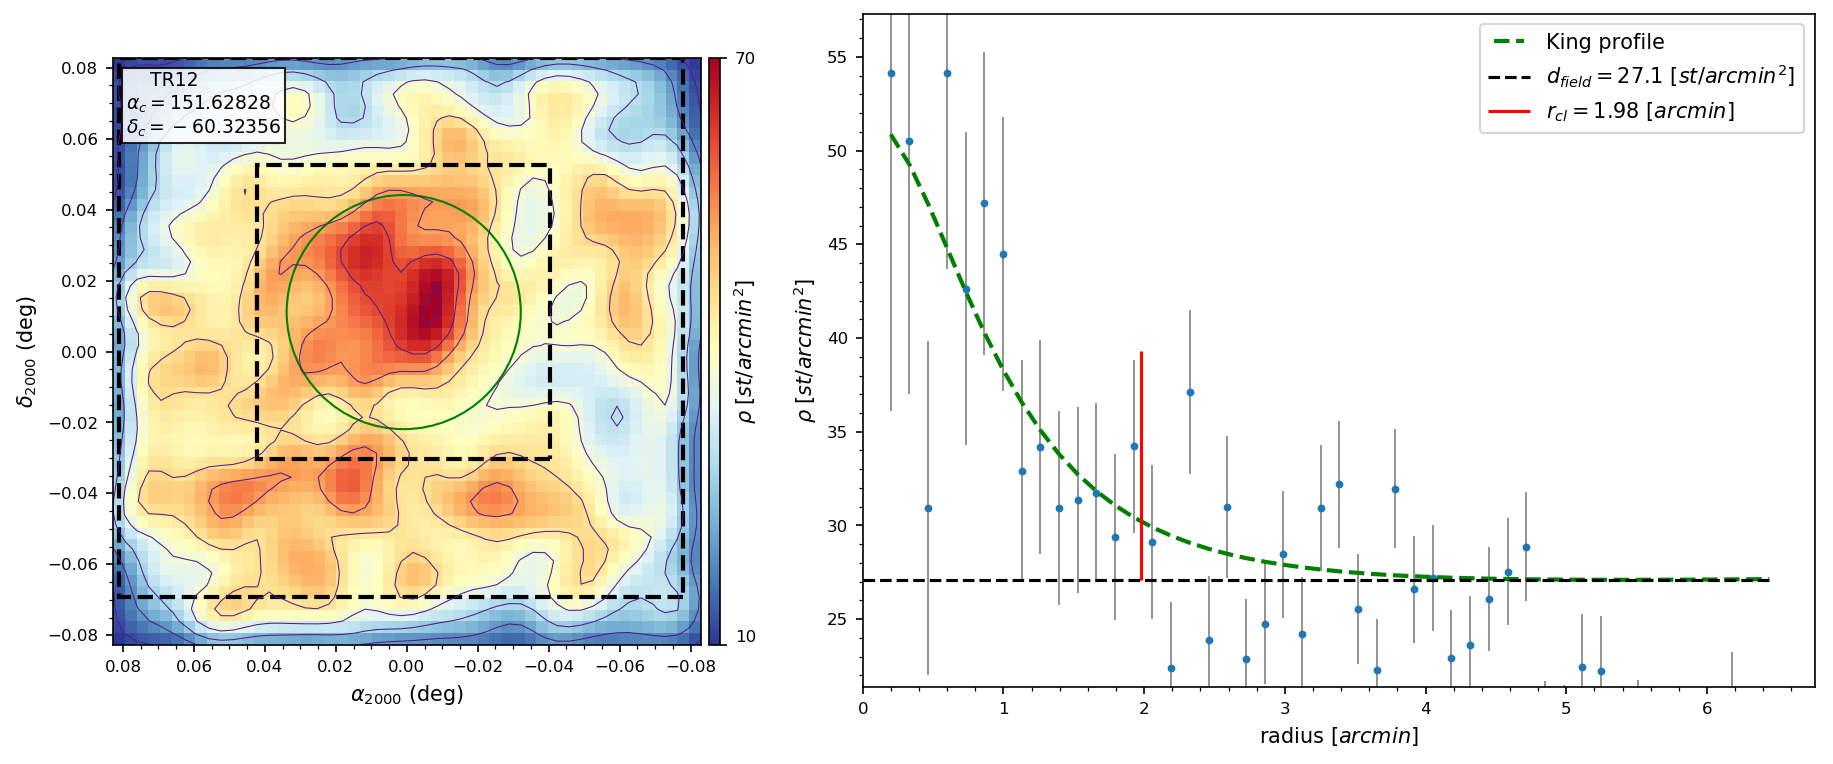
\includegraphics[width=\hsize]{../figs/dmap_trumpler12.png}
    \caption{Idem Fig. \ref{fig:struct_vdBH85} for TR 12.}
    \label{fig20}
\end{figure*}
\begin{figure*}[ht]
    \centering
    \includegraphics[width=\hsize]{../figs/cmds_tr12.png}
    \caption{Idem Fig. \ref{fig:fundpars_vdBH85} for TR 12.}
    \label{fig21}
\end{figure*}
\begin{figure*}[ht]
    \centering
    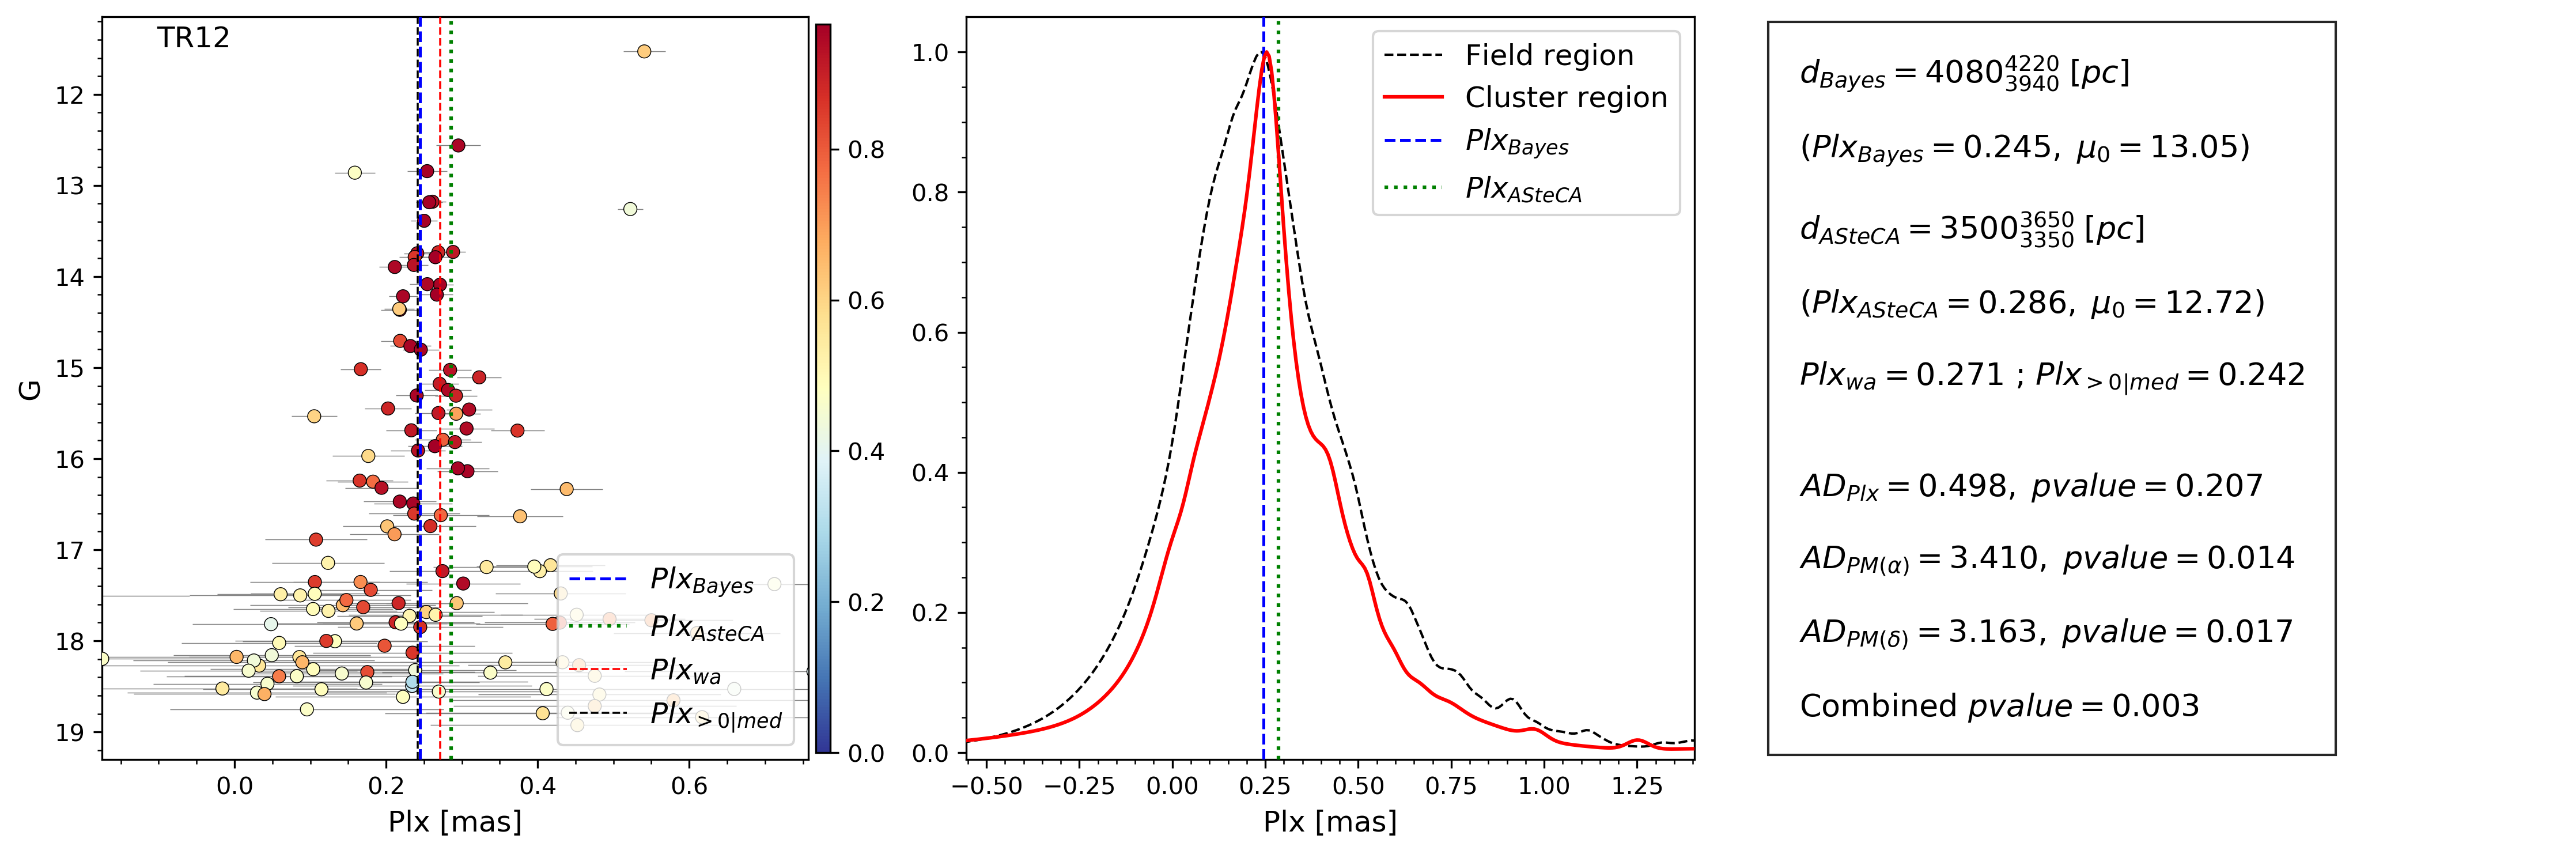
\includegraphics[width=\hsize]{../figs/plx_TR12.png}
    \caption{Idem Fig. \ref{fig:plx_bys_vdBH85} for TR 12.}
    \label{fig22}
\end{figure*}



%================================================================
\section{van den Bergh-Hagen 91}

vdBH 91 is a potential cluster at the west side of Carina HII
region, specifically, near the northern border of this constellation with Vela.
No relevant stellar structure appears in the $V$ image of Fig. \ref{fig:Vim},
but a common pattern of a Galactic field star near the Galactic plane.
The overall CMDs in Fig.~\ref{fig27} show a stellar sequence that at first
sight, resembles the usual diagrams for open clusters. In turn, the CCD
is dominated by a tail of $F$- and $G$-type stars prolonged by red stars. We also note some reddened early-type stars for negative
$(U-B)$ indices.\\

\texttt{ASteCA} found two well-separated stellar overdensity peaks in
Fig.~\ref{fig28}, whose relevance in terms of structure is not
important given the overall low stellar density of the field.
The noisy RDP by itself proves the poverty of the entire field we surveyed in terms
of star numbers.
After some attempts to search for a cluster sequence, we asked \texttt{ASteCA} to
estimate the probabilities for stars inside an adopted radius
of $\sim2.5$ arcmin, shown in Fig.~\ref{fig28} (right).
As shown in Fig.~\ref{fig29}, almost 100 stars inside the circle
associated with vdBH 91 were found in the CMDs.
No clear cluster sequence is traced by stars with high probabilities, which
are scattered across the entire CMD. The absence of a cluster sequence
combined with the poor and noisy overdensity all argue against the reliability of
this cluster.

The Anderson-Darling test in the right panel of Fig. \ref{fig30}, is clear regarding
the true nature of vdBH 91 because the high combined $p$-value
indicates that the null hypothesis (cluster and field areas come from the same
originating distribution) cannot be reasonably rejected. This result disgrees with the results
reported by \cite{Kharchenko_2005}, who found that vdBH 91
is a cluster at 0.75 kpc, approximately $0.16\times10^9$ yr old, and affected by
a mean color excess $E(B-V)=0.08$.\\

We conclude that vdBH 91 is a random fluctuation of the stellar
foreground and background, and not a real entity.

\begin{figure*}[ht]
    \centering
    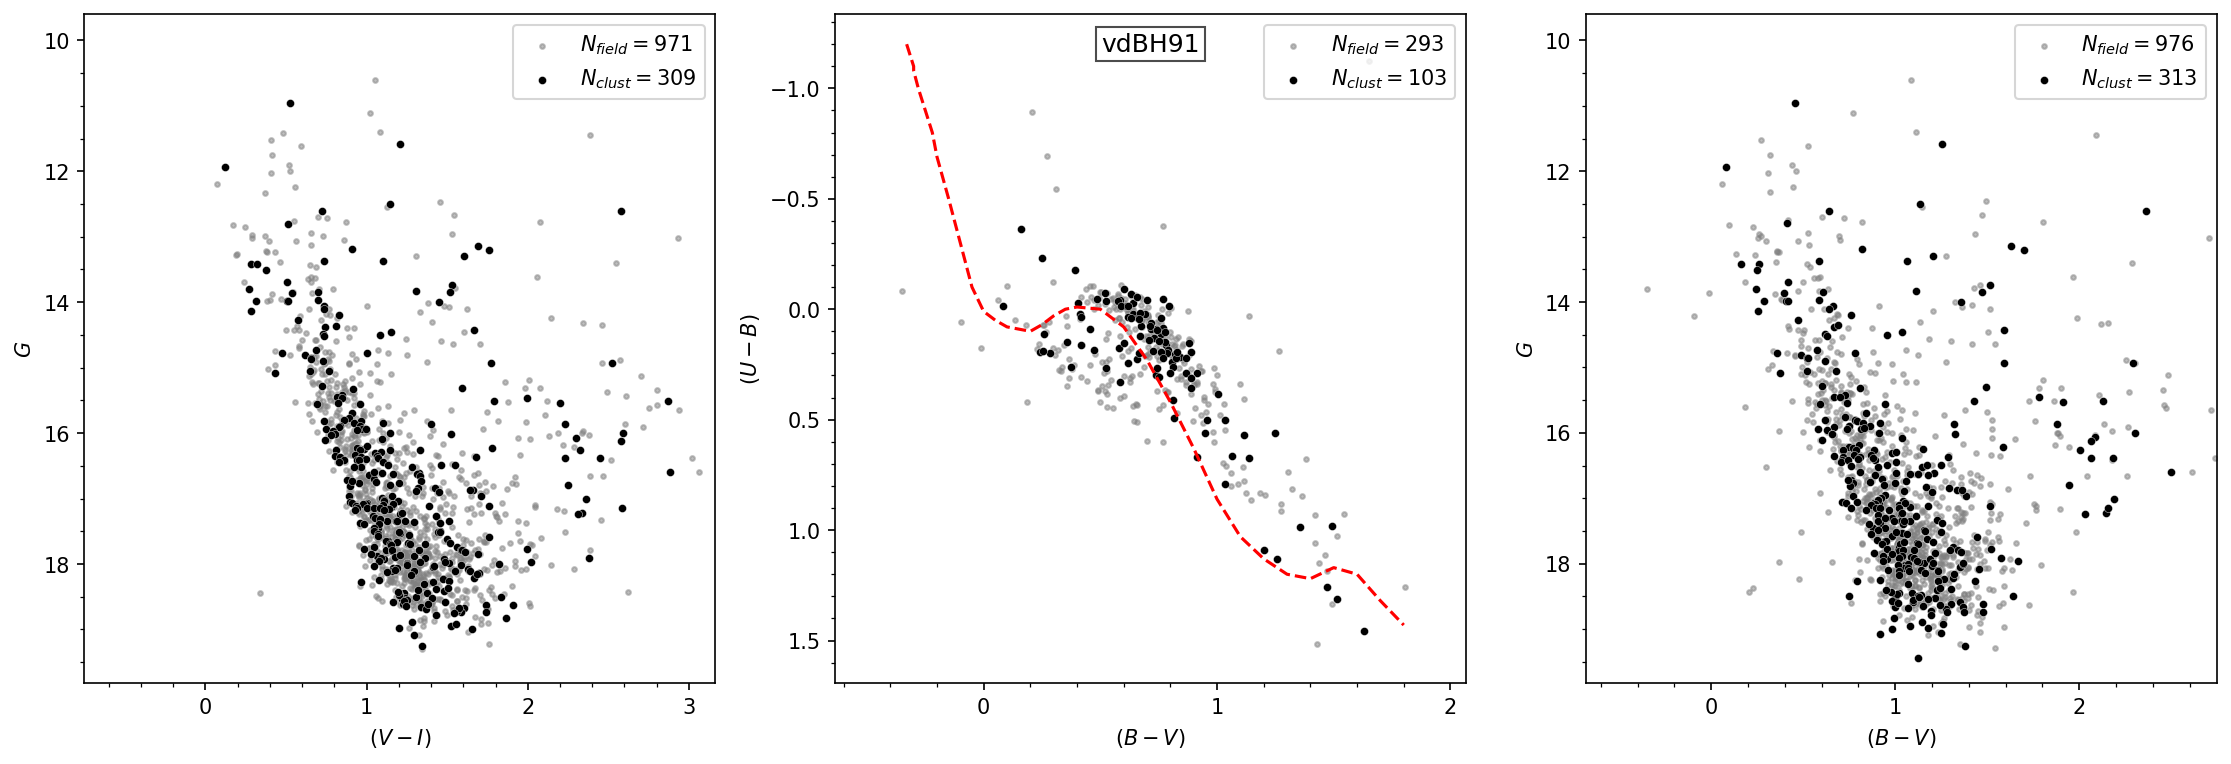
\includegraphics[width=\hsize]{../figs/obs_vdBH91.png}
    \caption{Idem Fig. \ref{fig:photom_vdBH85} for vdBH 91.}
    \label{fig27}
\end{figure*}
\begin{figure*}[ht]
    \centering
    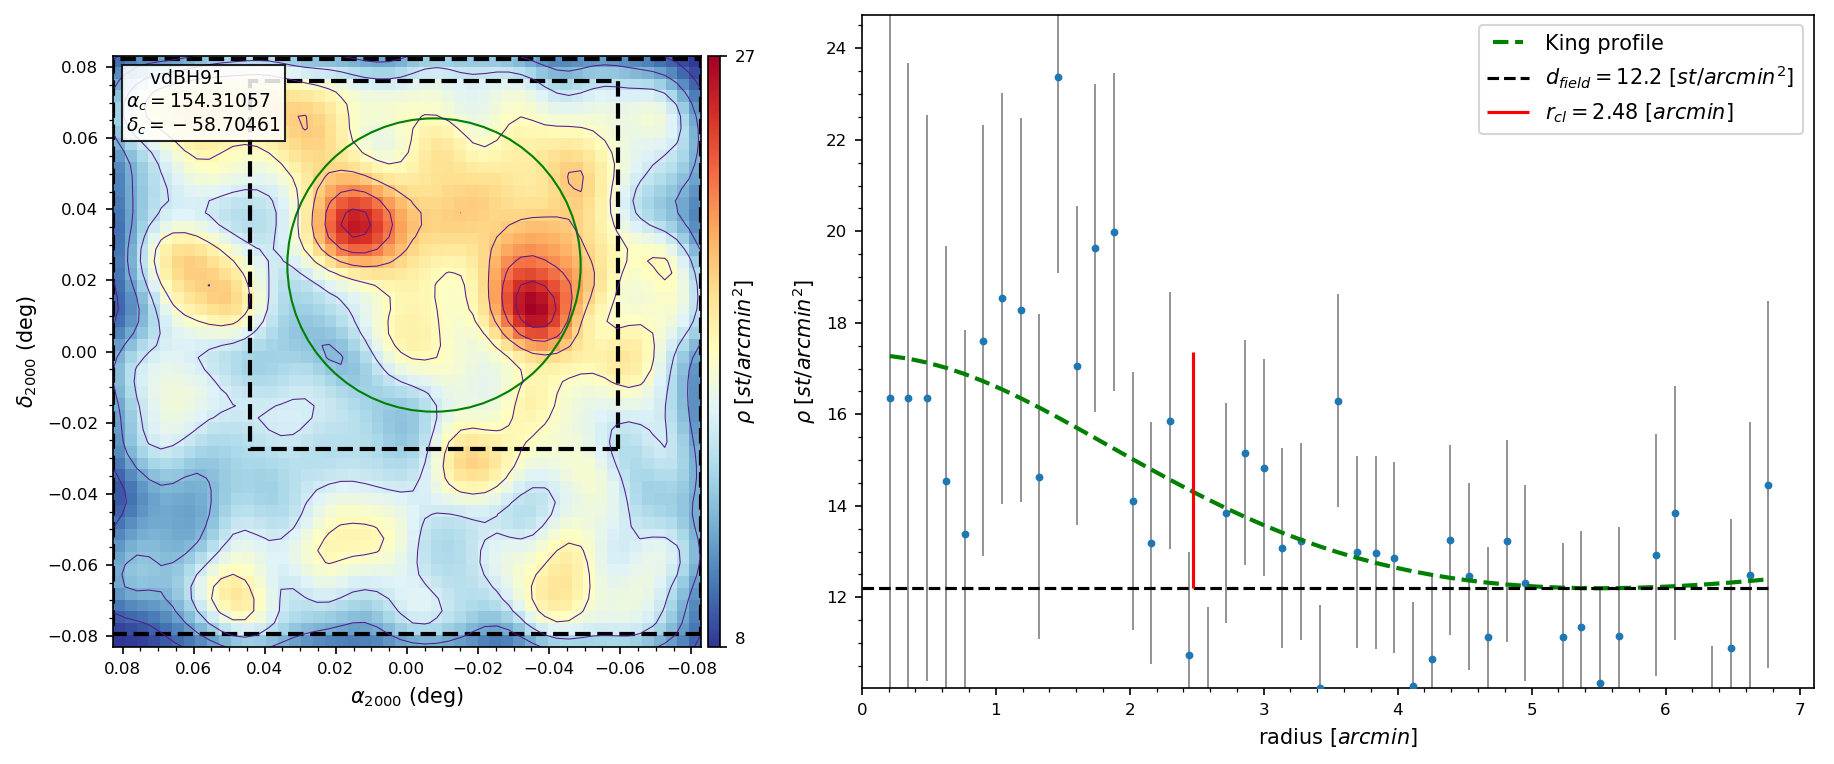
\includegraphics[width=\hsize]{../figs/dmap_vdbh91.png}
    \caption{Idem Fig. \ref{fig:struct_vdBH85} for vdBH 91.}
    \label{fig28}
\end{figure*}
\begin{figure*}[ht]
    \centering
    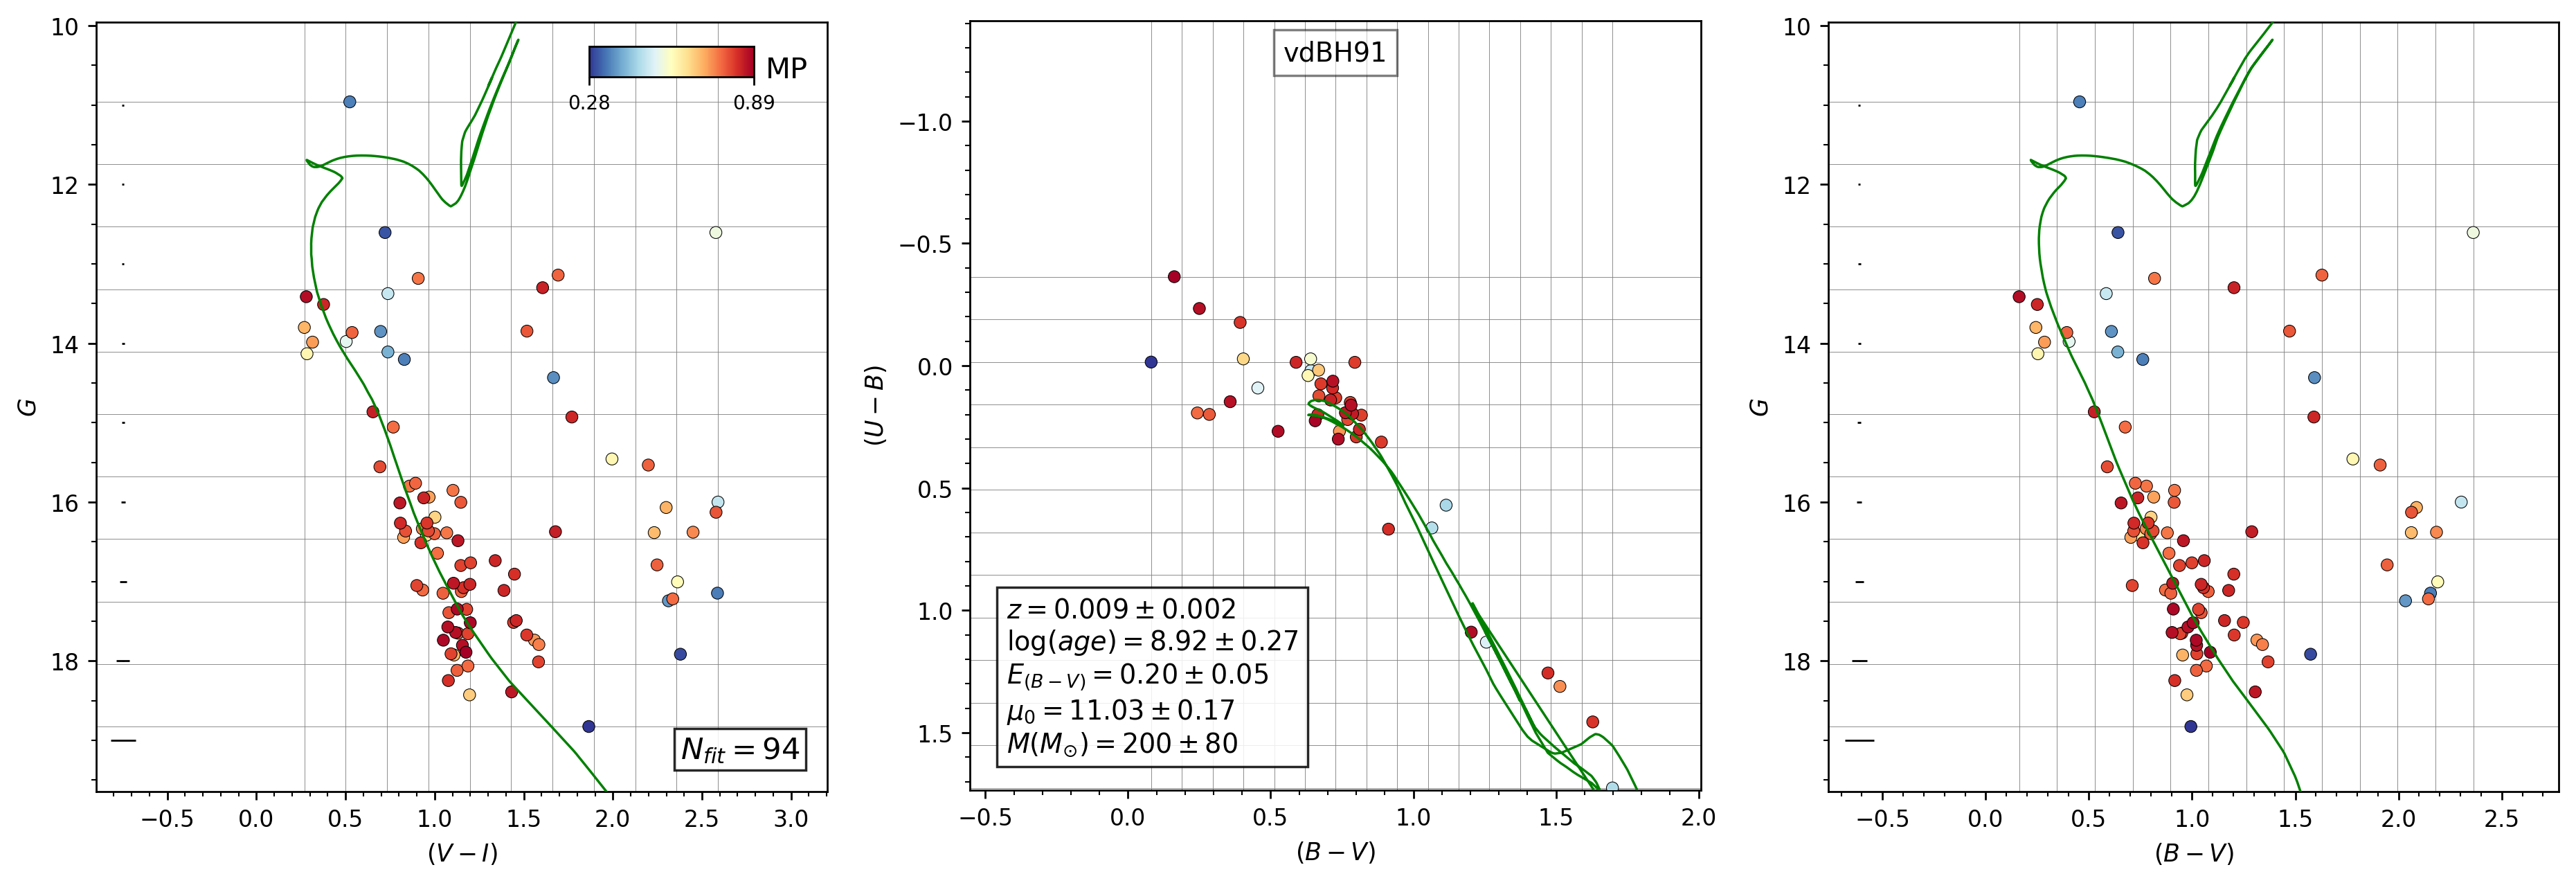
\includegraphics[width=\hsize]{../figs/cmds_vdBH91.png}
    \caption{Idem Fig. \ref{fig:fundpars_vdBH85} for vdBH 91.}
    \label{fig29}
\end{figure*}
\begin{figure*}[ht]
    \centering
    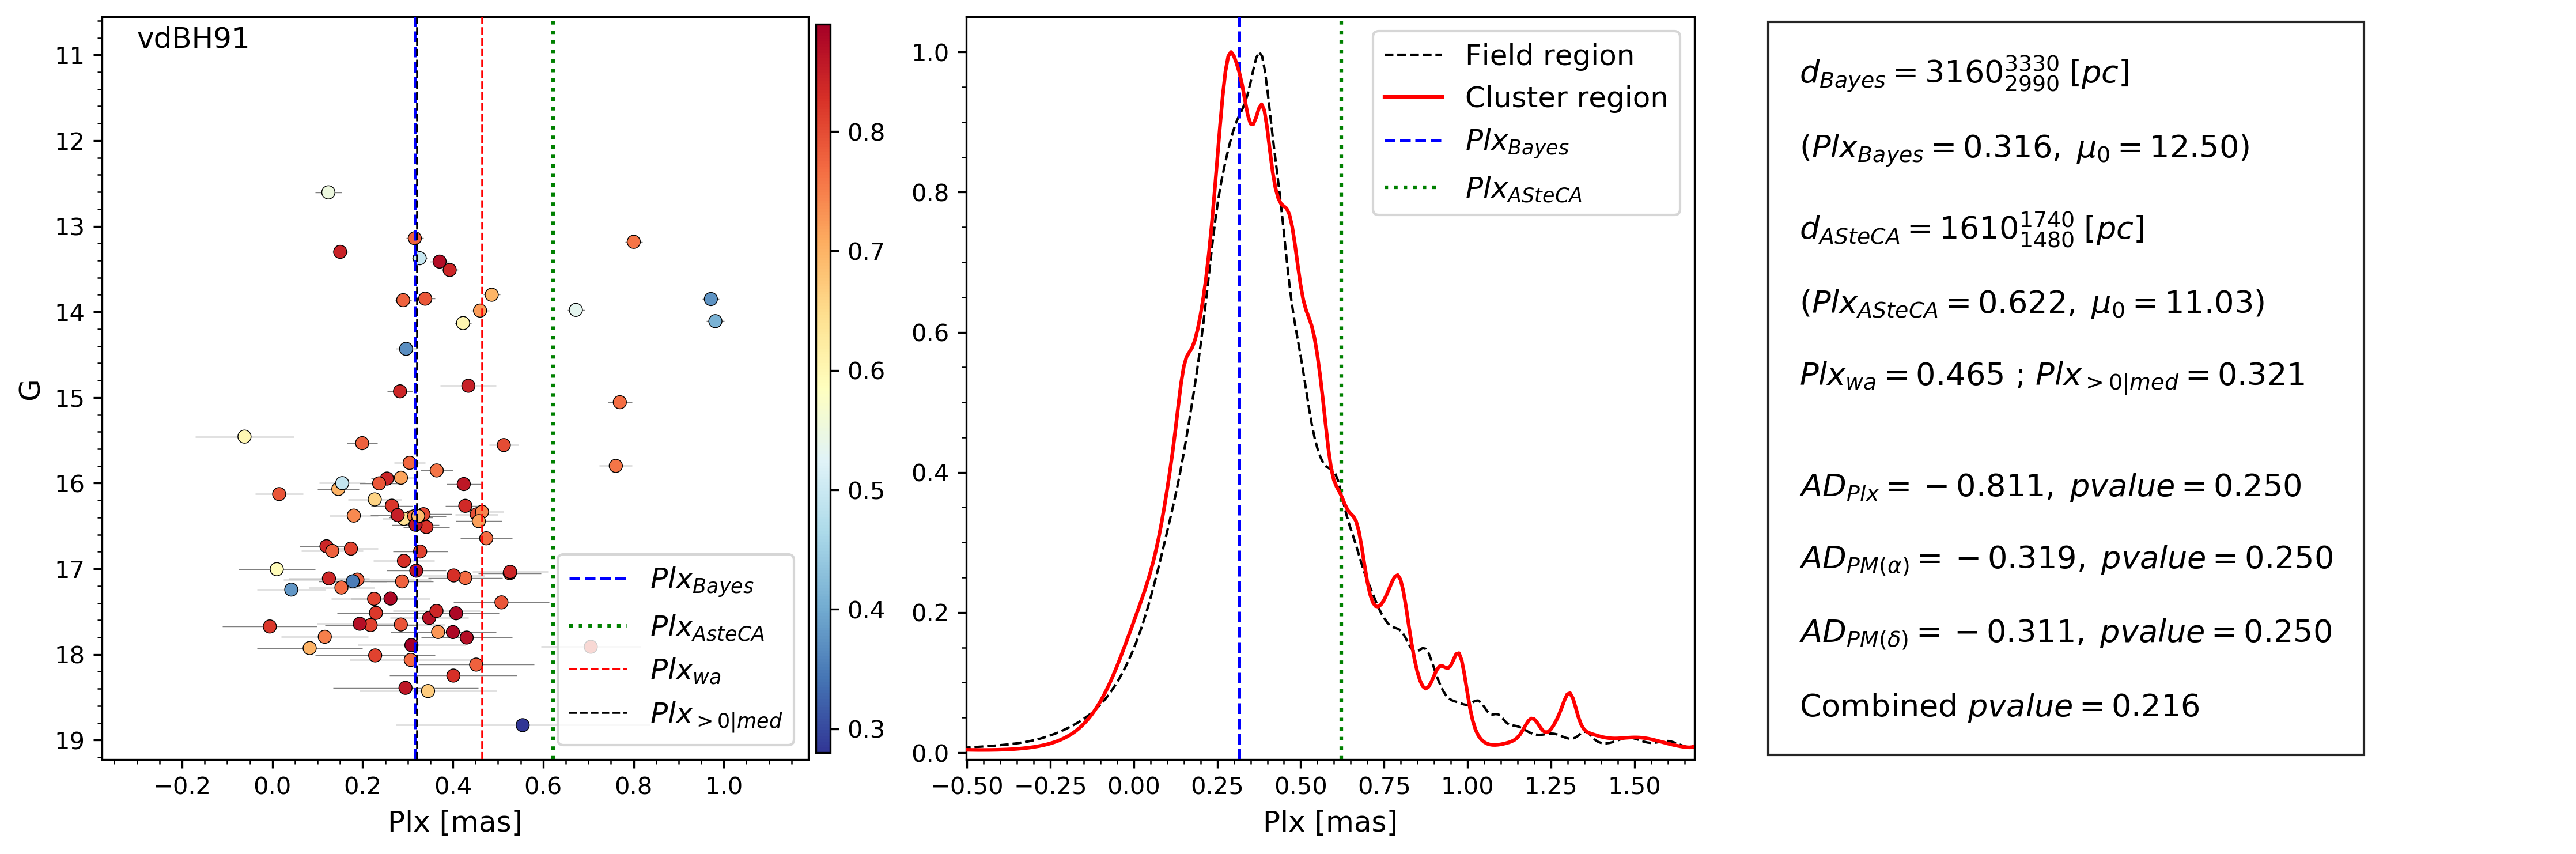
\includegraphics[width=\hsize]{../figs/plx_vdBH91.png}
    \caption{Idem Fig. \ref{fig:plx_bys_vdBH85} for vdBH 91.}
    \label{fig30}
\end{figure*}



%================================================================
\section{Trumpler 13}

TR 13 is a weak object also at the southwest of the Carina HII
region, seen as a diffuse but extended stellar accumulation near the center of the
$V$ image in Fig.~\ref{fig:Vim}. The two CMDs in Fig. \ref{fig39} show an
uncommon pattern:  above $G=17.5$ mag, the stellar sequence splits
into two branches, one of which extends to the bluest side, while the other
branch follows the common representation of galaxy disk stars. The situation is the same in the CCD: a wide and reddened band of potential
$B$-type stars is placed at $(B-V)<0.45$ and $-0.25<(U-B)<0.5,$ with a few
more stars at  the negative $(U-B)$ index, while another strip of stars extends from the
characteristic place for $F$-type stars and reaches the red tail, including
probable giant stars.\\

Fig. \ref{fig40} indicates that \texttt{ASteCA} found a spatially extended
overdensity mostly elongated north-south, which is nearly four times
above a mean field stellar density of $\sim26$ stars per square arcminutes at
its peak. Based on the shape and extension of the overdensity, we adopted a
formal radius of $\sim2.5$ arcmin and asked \texttt{ASteCA} to compute the
membership probabilities for the stars inside the area. 
Fig. \ref{fig41} shows that after field interlopers are removed, almost 170
stars are left composing a narrow cluster main sequence that extends for more than
five magnitudes. Consequently, when we compare this with synthetic clusters,
the results yield

\begin{itemize}
\item [a)] a color excess of $E(B-V)=0.56$  for the best fit
of a synthetic cluster. Because the maximum color excess provided by S\&F2011
is 1.94, it is reasonable to conclude that most of the absorption is produced
behind the position of TR 13.
\item [b)] that the absorption-free distance modulus of TR 13 is estimated to be
$13.41\pm0.15$ mag, placing it at a distance of $4.81\pm0.33$ kpc from
the Sun.
\end{itemize}

The Anderson-Darling statistics in the right panel of Fig.~\ref{fig42} confirms the
photometric results: cluster area and the surrounding field region
possess quite different properties.\\

The selected probable members inside the overdensity confirm the
true nature of this object because the over density and the density profile are
followed by a very well defined and extended photometric counterpart. All these
facts combined with the results from the Anderson-Darling test are
self-consistent, so that we are confident that TR 13 is a young cluster of
$0.11\pm0.02\times10^9$ years.

\begin{figure*}[ht]
    \centering
    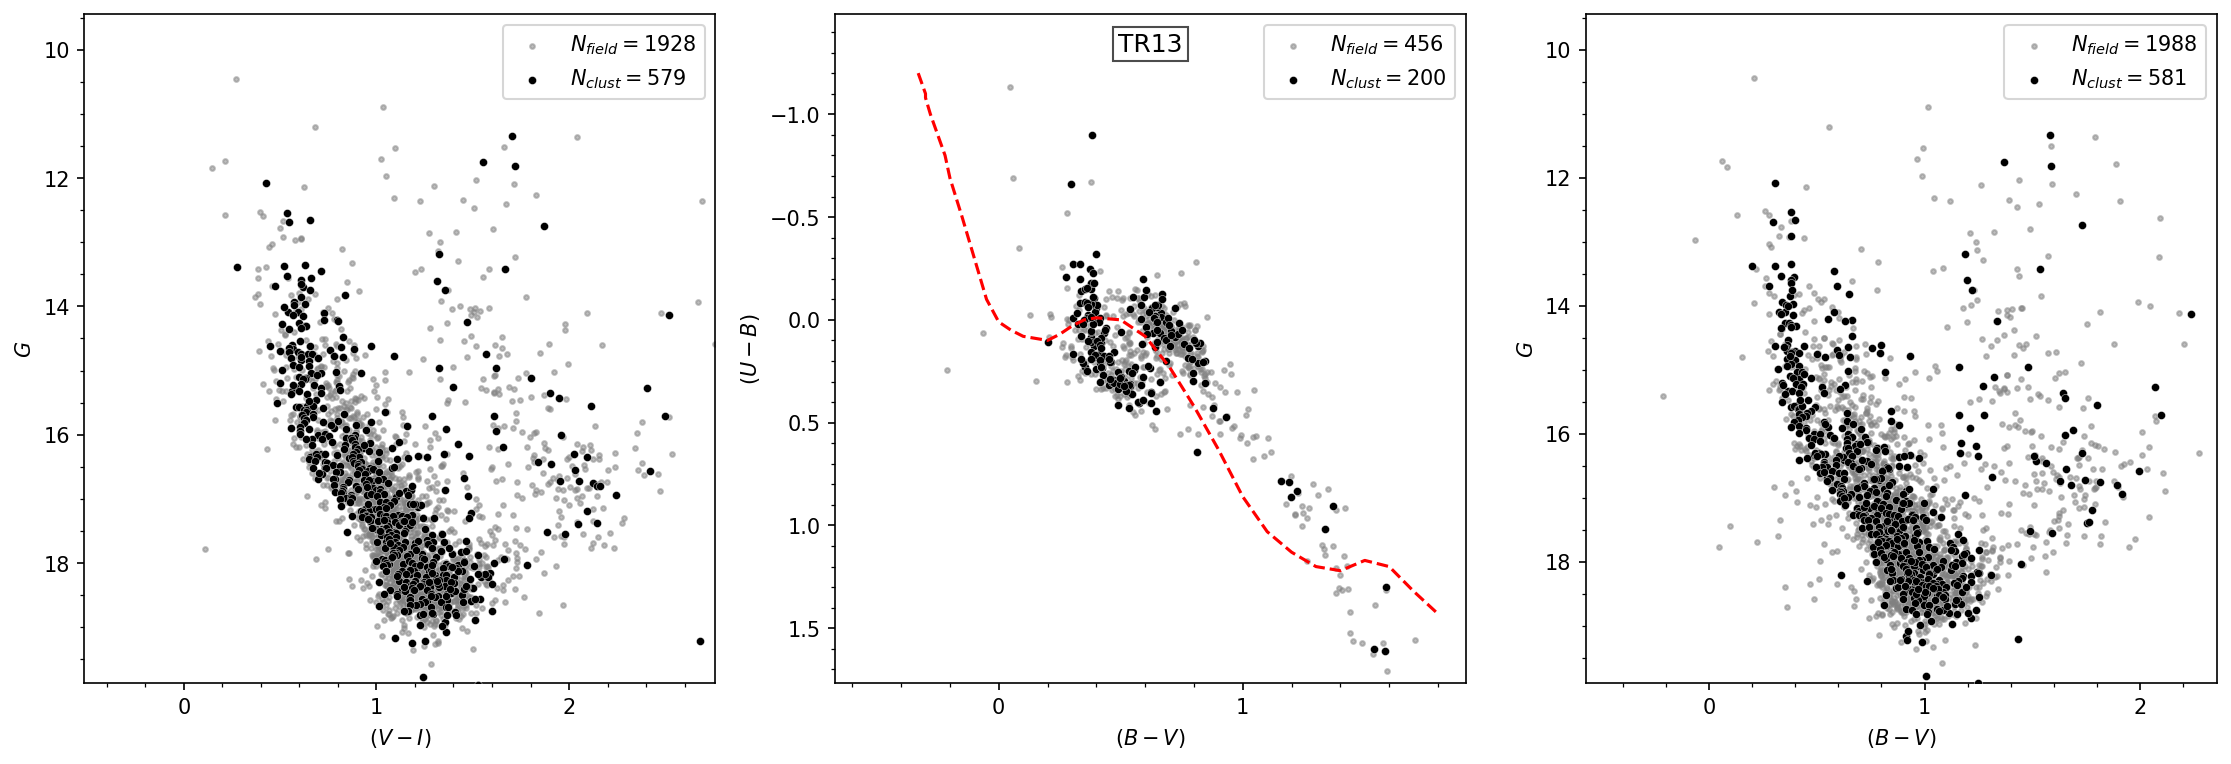
\includegraphics[width=\hsize]{../figs/obs_TR13.png}
    \caption{Idem Fig. \ref{fig:photom_vdBH85} for TR 13.}
    \label{fig39}
\end{figure*}
\begin{figure*}[ht]
    \centering
    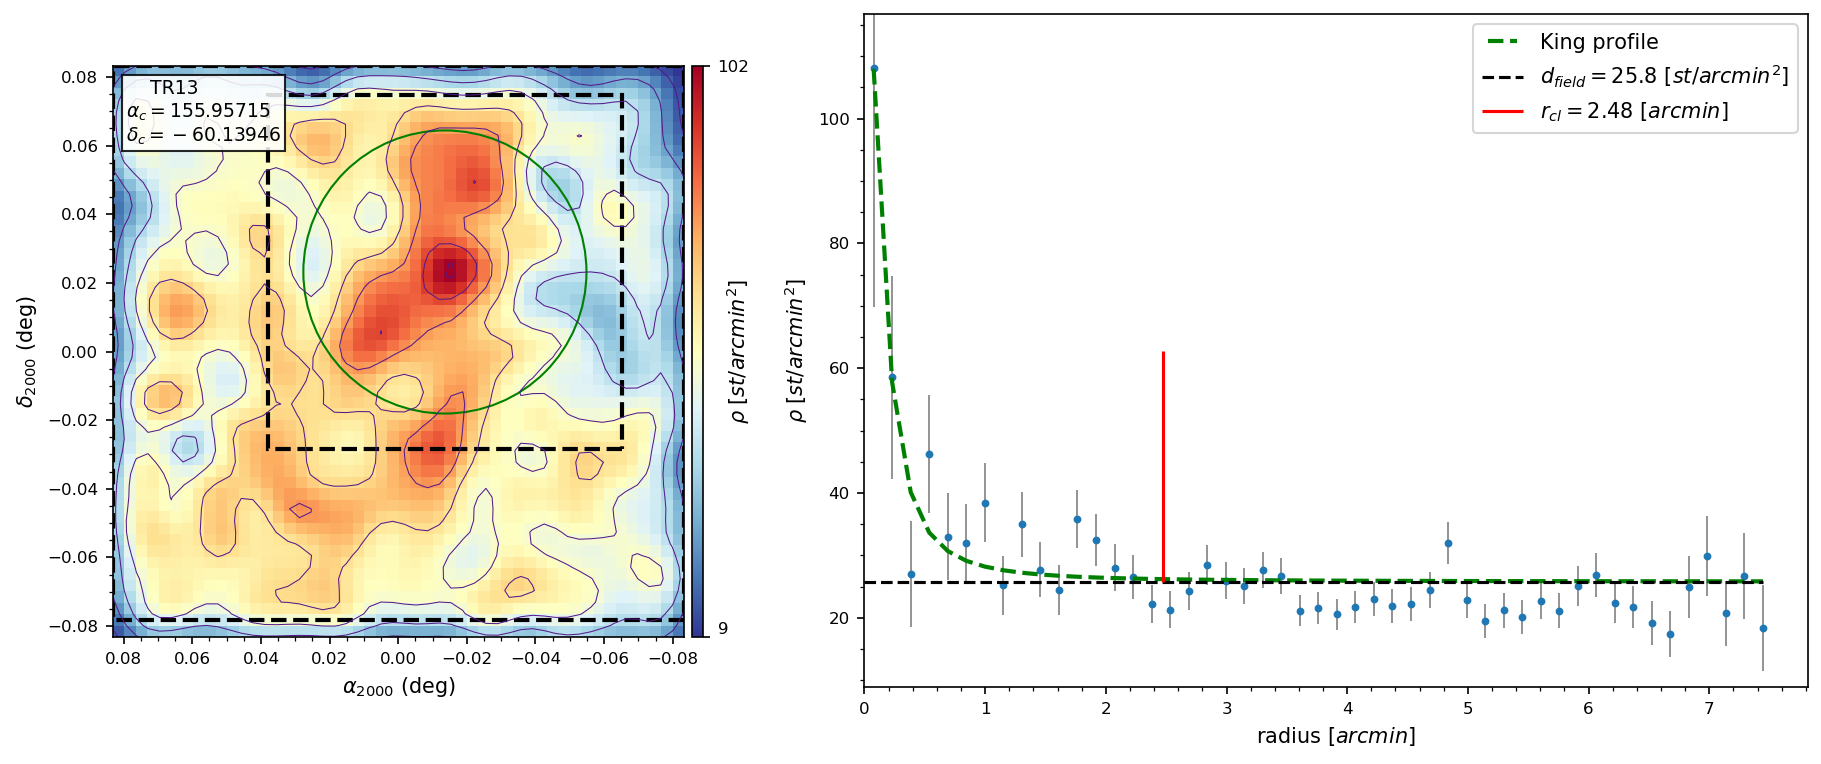
\includegraphics[width=\hsize]{../figs/dmap_trumpler13.png}
    \caption{Idem Fig. \ref{fig:struct_vdBH85} for TR 13.}
    \label{fig40}
\end{figure*}
\begin{figure*}[ht]
    \centering
    \includegraphics[width=\hsize]{../figs/cmds_tr13.png}
    \caption{Idem Fig. \ref{fig:fundpars_vdBH85} for TR 13.}
    \label{fig41}
\end{figure*}
\begin{figure*}[ht]
    \centering
    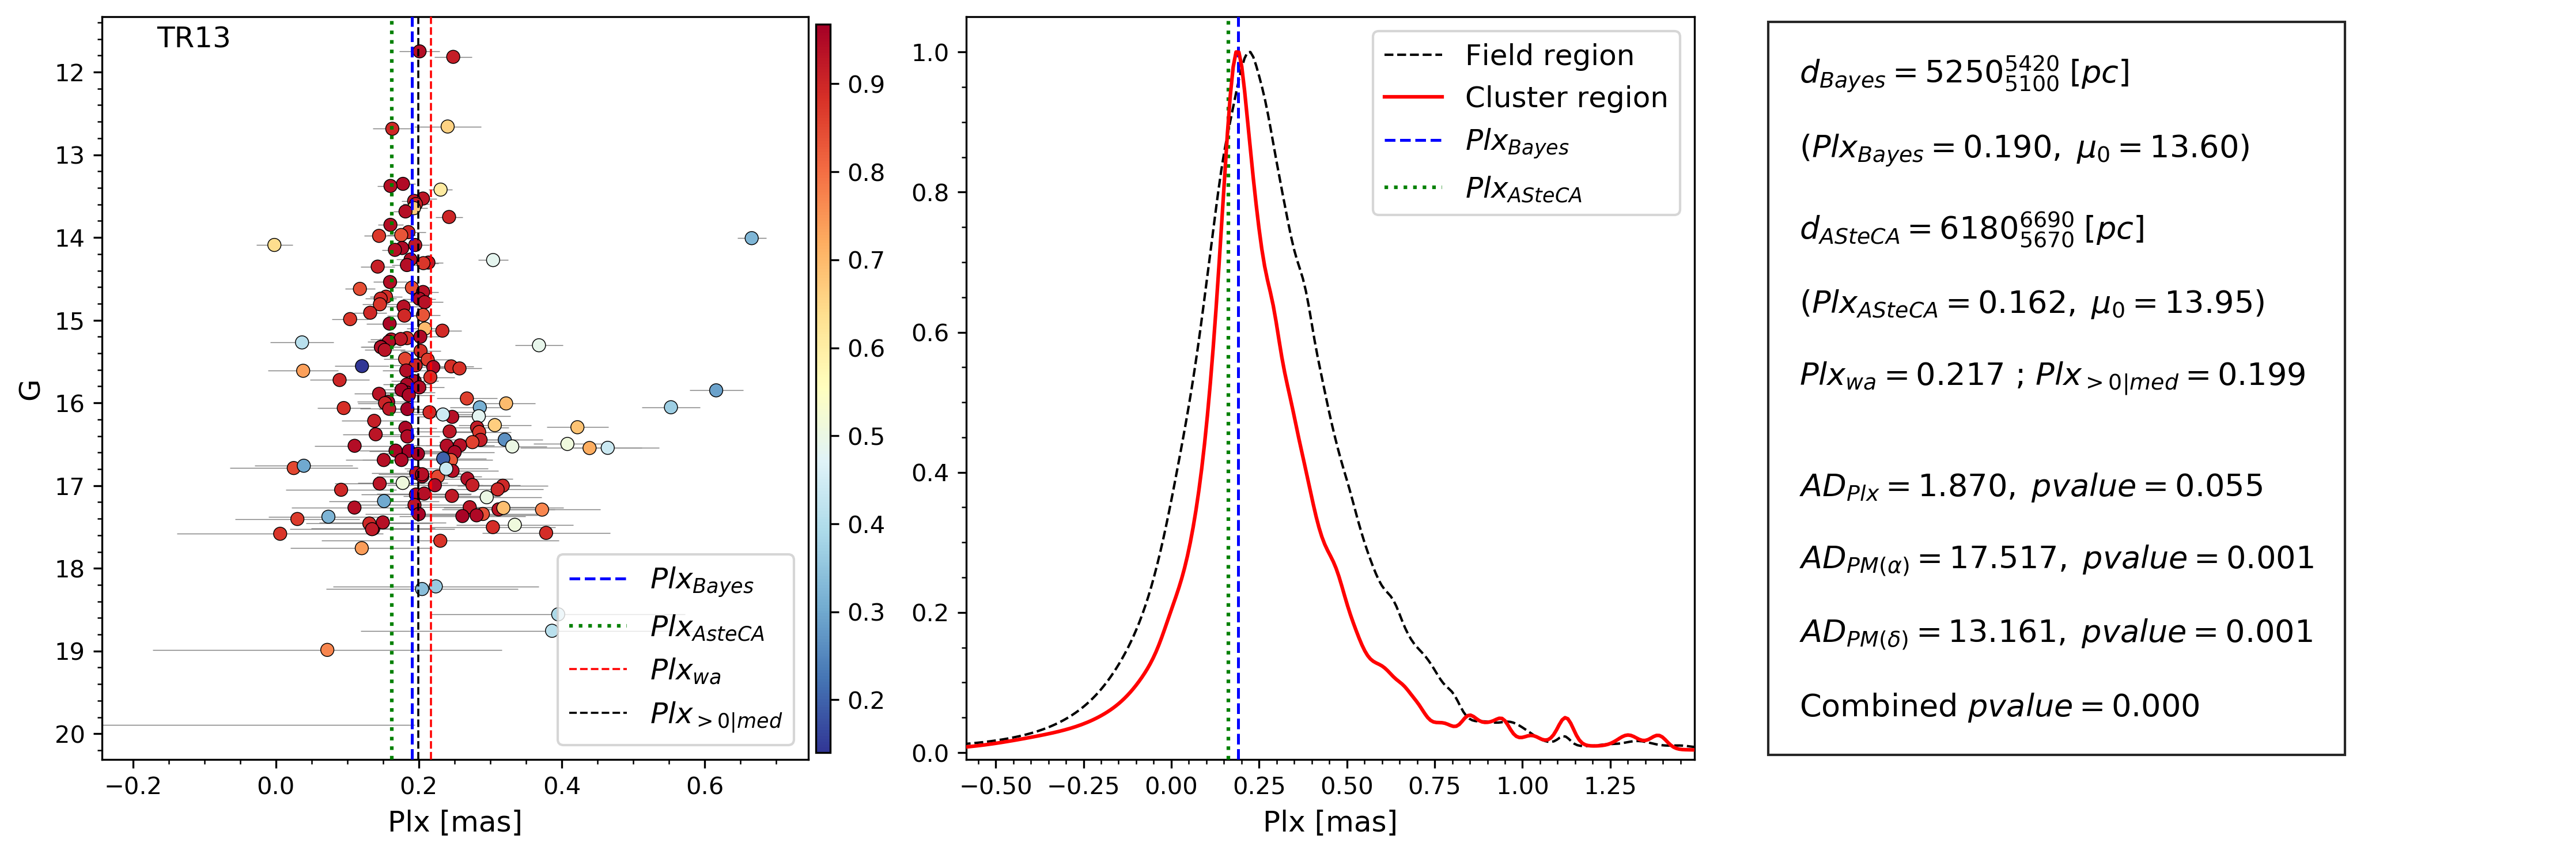
\includegraphics[width=\hsize]{../figs/plx_TR13.png}
    \caption{Idem Fig. \ref{fig:plx_bys_vdBH85} for TR 13.}
    \label{fig42}
\end{figure*}




%================================================================
\section{van den Bergh-Hagen 106}

This cluster is placed at the southeast of the Vela constellation. The stellar field where it is placed is not very dense and has no relevant features, except for a few
moderately bright stars, as shown in Fig. \ref{fig:Vim}.
The CMDs shown in Fig.~\ref{fig43} represent typical photometric features:
structures of Galactic fields with no cluster inside. The CCD in the
same figure shows a reduced number of stars below the intrinsic line 
(probably reddened late $B$- and $A$-types) and a tail of stars from of late
$F$-types to $M$-type stars, some of them probably giants, at the red end.
The %
\texttt{ASteCA} spatial analysis found some stellar clumps, as shown in the left panel of
Fig.~\ref{fig44}. We focus on the main clump at the very
center of the frame because here we see the highest overdensity peak with
$\text{about three}$ times more stars than at the mean stellar background density of
$\text{about }11$ stars per square arcmin.
We assume that most of stars in vdBH 106 must be included there, so that the cluster
parameters are expected to be well established. The RDP to the right appears poorly
defined because it reflects the irregular and low stellar density even inside the
zone we selected to investigate the cluster parameters.
Only 82 stars were selected as probable members inside this area.
Stars whose probabilities are near the maximum values in this region would
seem to outline a (rather noisy) cluster sequence that can be fit with a
synthetic cluster. This yields the following parameters:

\begin{itemize}
\item [a)] A color excess of $E(B-V)=0.30$ was found to affect the
cluster. This value agrees well with the maximum color excess provided
by S\&F2011, $E(B-V)=0.57,$ in this direction.
\item [b)] The absorption-free distance modulus of vdBH 106 was found to be
$13.44\pm0.36$ mag, which places the cluster at a distance of
$d=4.87\pm0.81$ kpc from the Sun.
\end{itemize}

In this region we found by applying the Anderson-Darling test that
the parallax and proper motion distributions seem to belong to the same
originating distribution, as shown in Fig. \ref{fig46}. The
high combined $p$-value makes the rejection of the null hypothesis difficult
if not impossible\\

Although a trace of a sequence belonging to a typical old cluster is
noticeable in Fig.~\ref{fig45}, we are cautious to confirm its nature.
Clearly, deeper photometric observations (particularly in the $U$ filter) are
needed. Meanwhile, and assuming that it is a true object,
vdBH 106 might be an old open cluster that is about $3.00\pm0.80\times10^9$ years
old.

\begin{figure*}[ht]
    \centering
    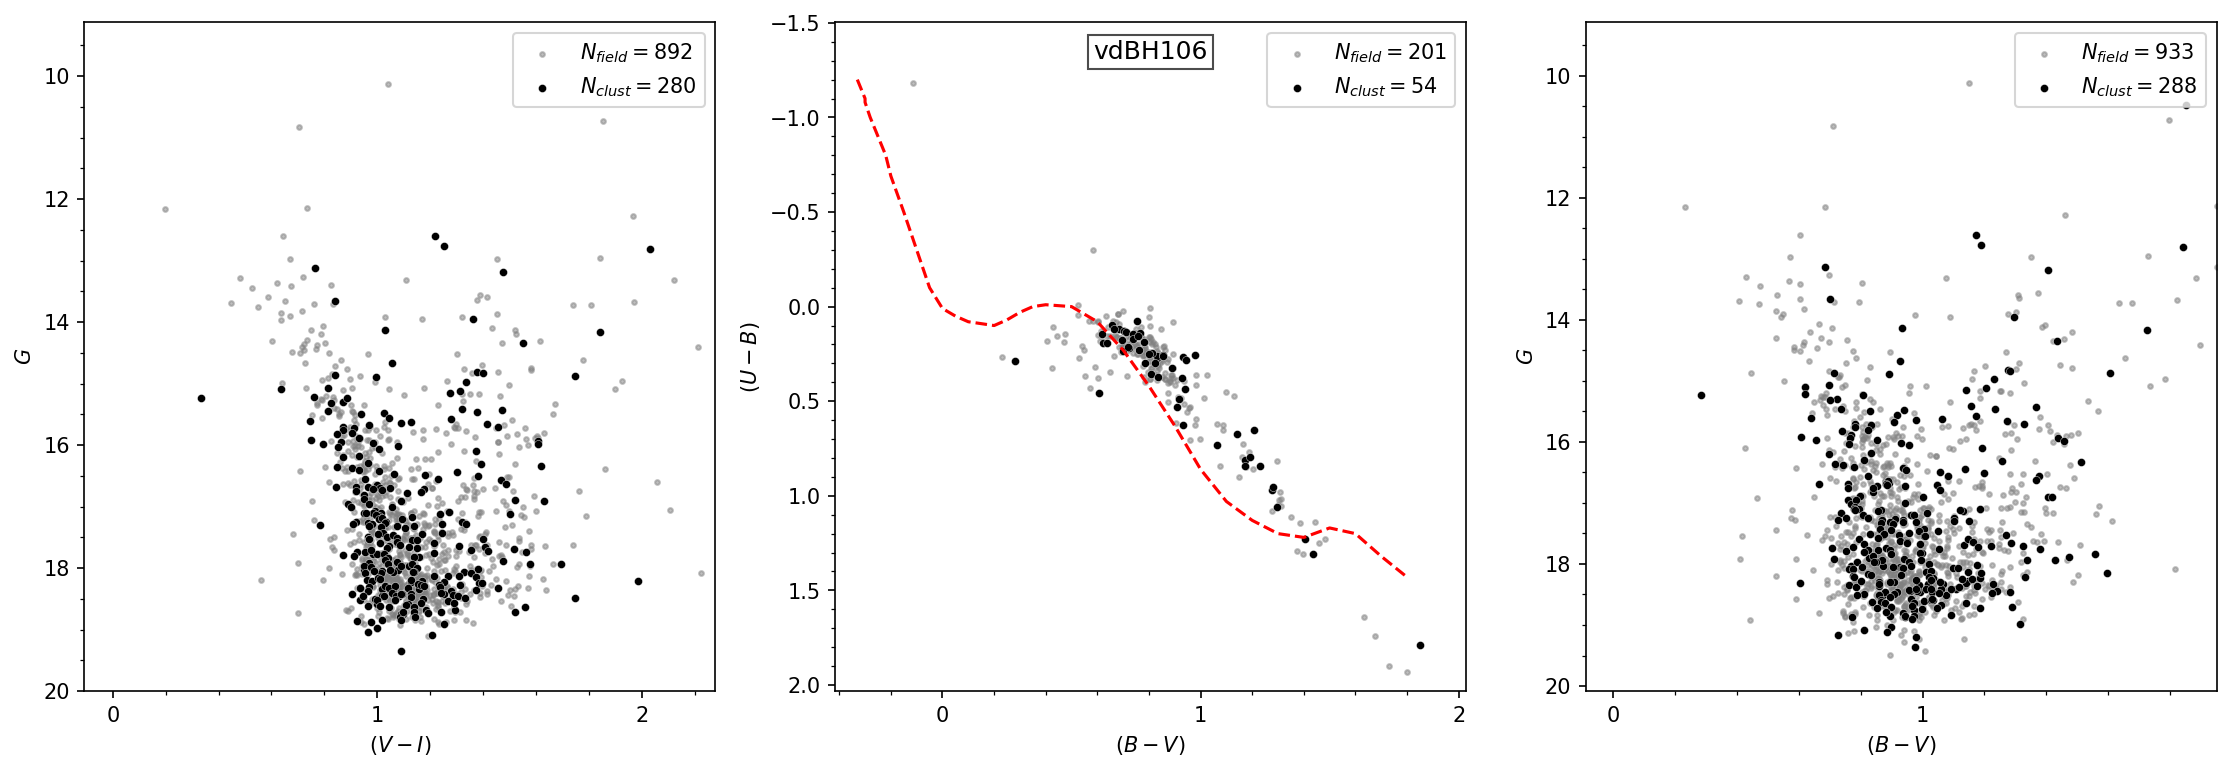
\includegraphics[width=\hsize]{../figs/obs_vdBH106.png}
    \caption{Idem Fig. \ref{fig:photom_vdBH85} for vdBH 106.}
    \label{fig43}
\end{figure*}
\begin{figure*}[ht]
    \centering
    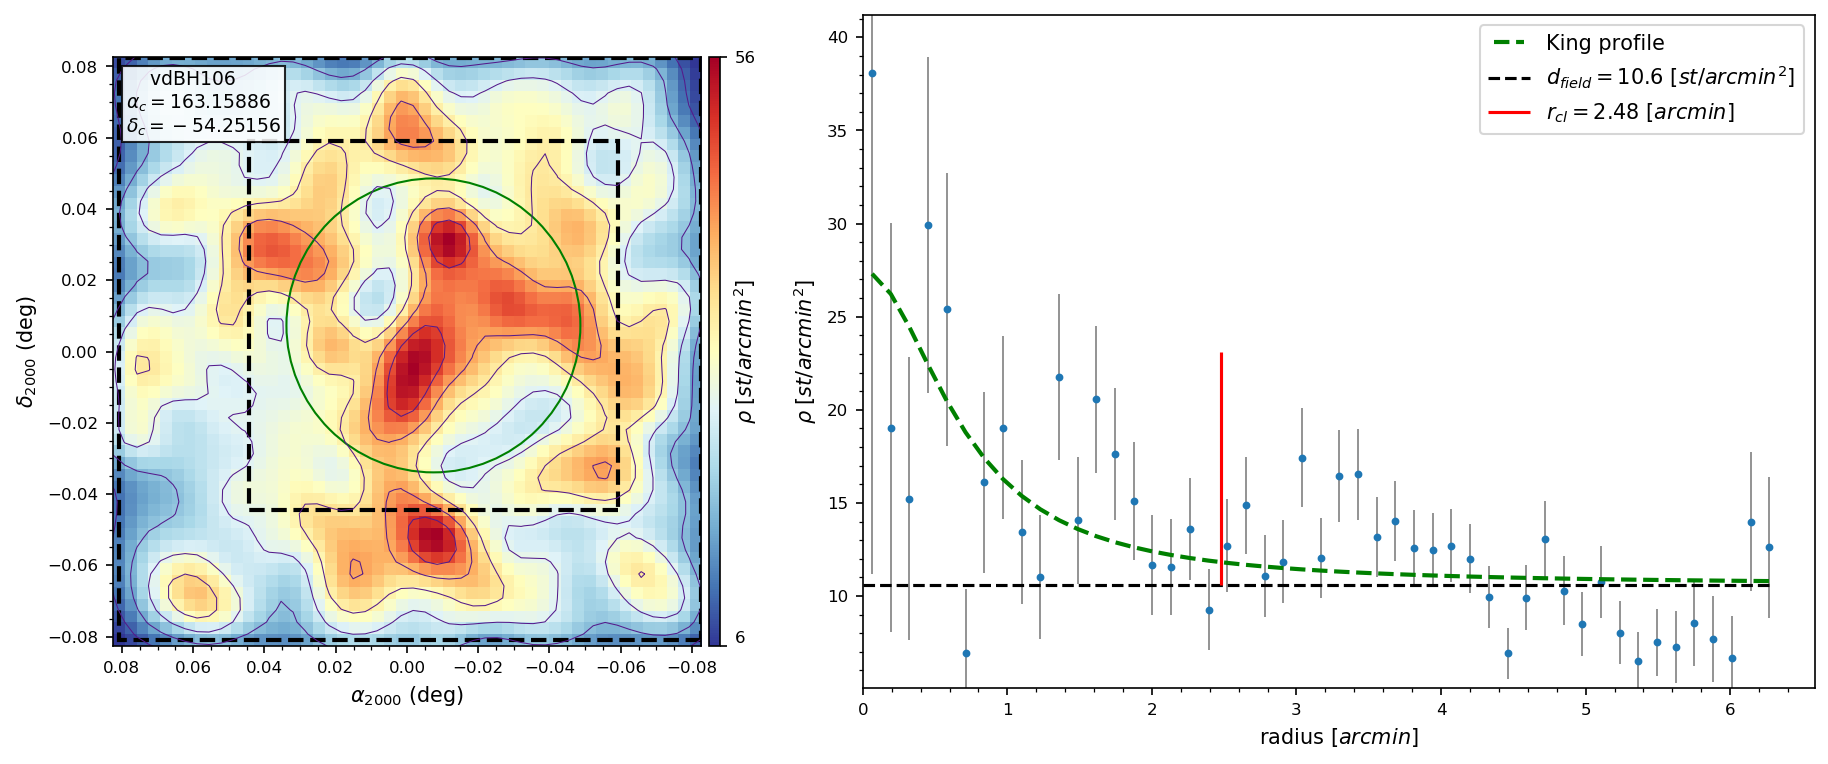
\includegraphics[width=\hsize]{../figs/dmap_vdbh106.png}
    \caption{Idem Fig. \ref{fig:struct_vdBH85} for vdBH 106.}
    \label{fig44}
\end{figure*}
\begin{figure*}[ht]
    \centering
    \includegraphics[width=\hsize]{../figs/cmds_vdbh106.png}
    \caption{Idem Fig. \ref{fig:fundpars_vdBH85} for vdBH 106.}
    \label{fig45}
\end{figure*}
\begin{figure*}[ht]
    \centering
    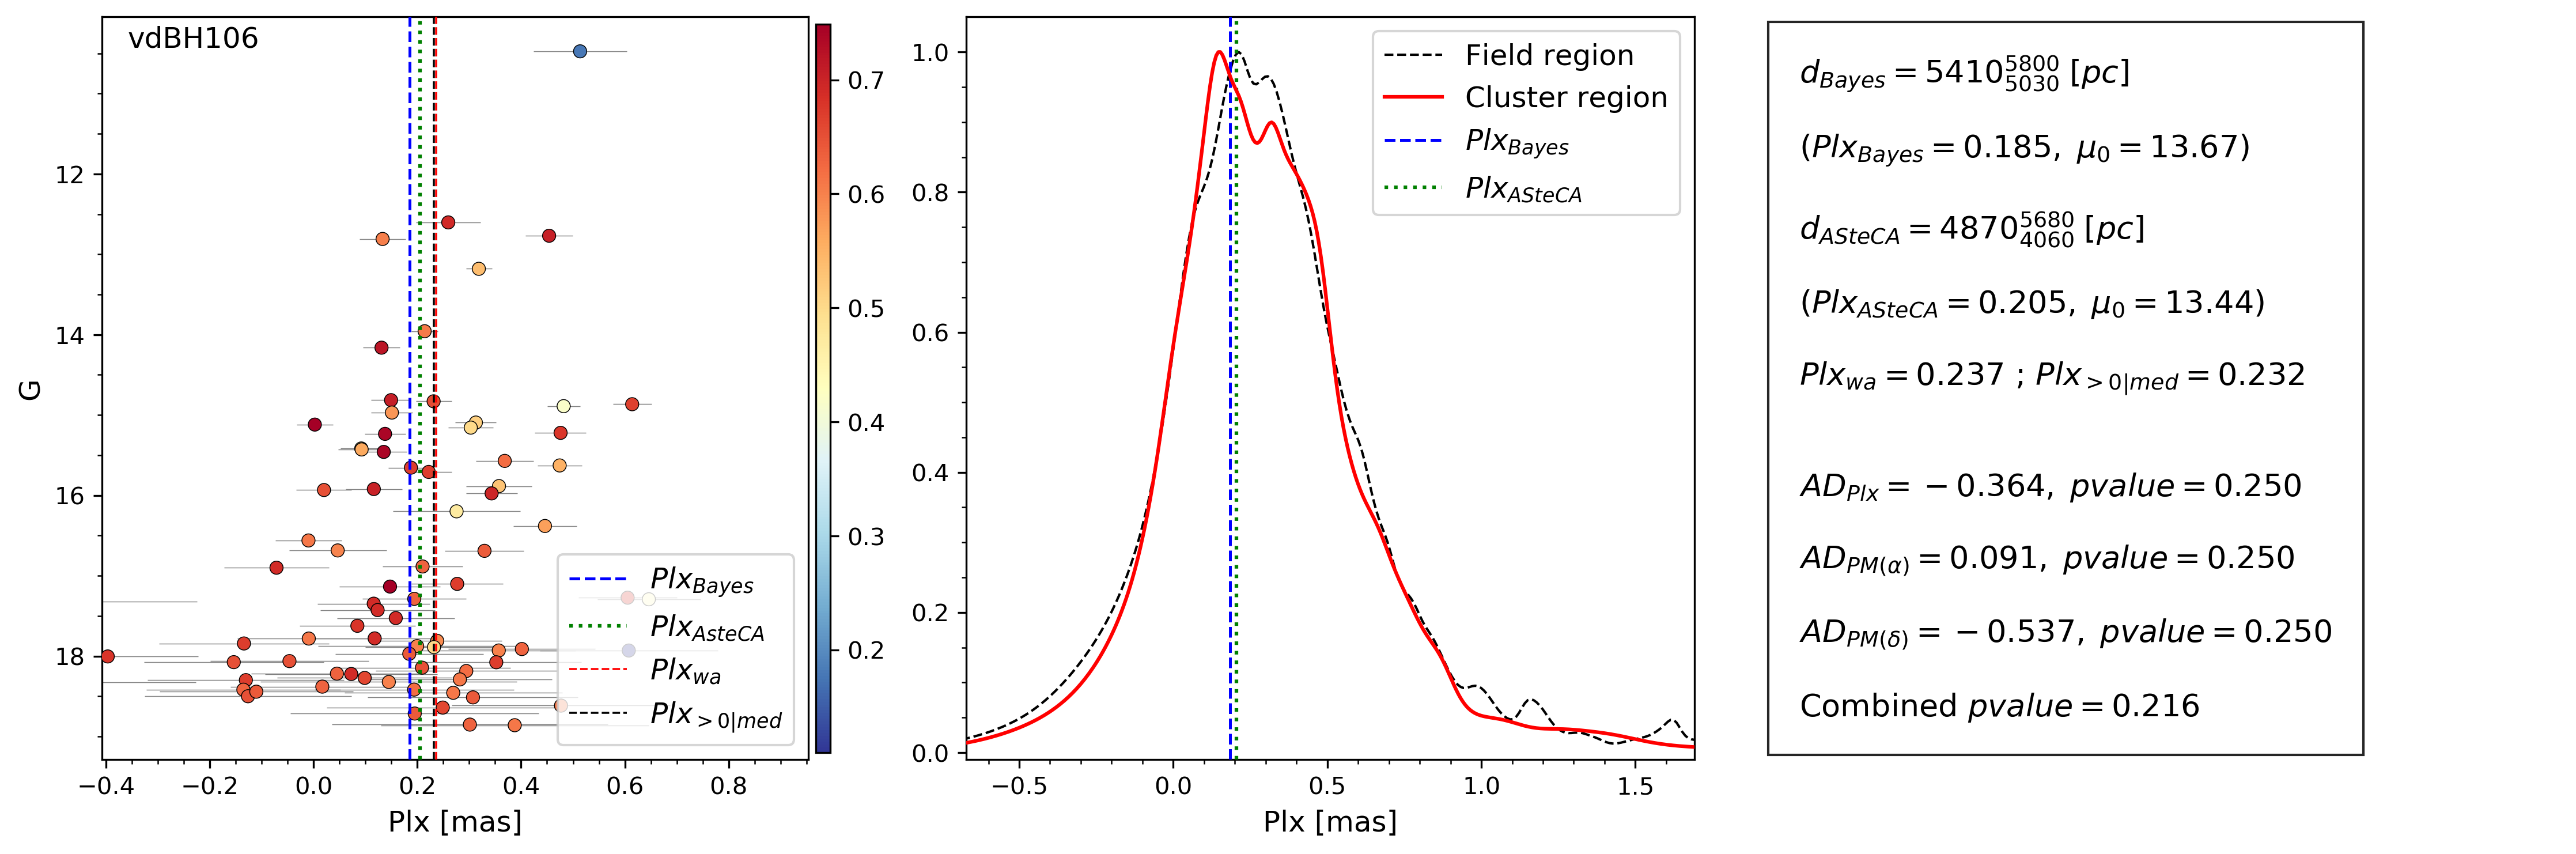
\includegraphics[width=\hsize]{../figs/plx_vdBH106.png}
    \caption{Idem Fig. \ref{fig:plx_bys_vdBH85} for vdBH 106.}
    \label{fig46}
\end{figure*}



%================================================================
\section{Ruprecht 88}

RUP 88 is another potential cluster south of the Carina HII region. Like
other objects in this paper, no obvious stellar grouping is perceived in the $V$
image of Fig. \ref{fig:Vim}. The overall stellar CMDs in Fig.~\ref{fig31} show a
scattered stellar distribution above $G=16$ mag. From this magnitude down the
common pattern of galactic disk stars takes place in the CMDs. The CCD in Fig.
\ref{fig31} suggests that no blue and therefore young star is present in the
region of RUP 88. In the range $0.2<(B-V)<0.8,$  a handful of stars might be reddened late $B$- types or $A$-$F$-type stars. The remainder of
this diagram is a trace composed of $A$- to $M$-type stars.\\

As with other clusters in the present sample, when the spatial distribution
of stars in the frame is analyzed, no clear stellar overdensity
appears in the location where RUP 88 is assumed to be located. The
contour plot in the left panel of Fig. \ref{fig32} shows a weak enhancement in star number from southwest to northeast of the frame extending northwest.
Because it was difficult to state the position of the cluster center (if it
exists), we asked \texttt{ASteCA} to inspect the region encircled in green in Fig.
\ref{fig32}, where a reasonable density profile could be found. The
RDP is still noisy because of a rather low star number contained between the
assumed cluster limits.
The CMDs in Fig.~\ref{fig33} show that only 42 stars with a wide
range of probabilities remain inside the adopted cluster region 
after interlopers are removed, with no trace of a cluster sequence.
The three photometric diagrams in Fig. \ref{fig33} confirm this point: only
an amorphous distribution of stars that scarcely resembles a cluster main sequence
is visible.\\

The Anderson-Darling test in the right panel of Fig. \ref{fig34} cannot
separate the cluster population from the field region population for the
three dimensions. The combined $p$-value for proper motions and
parallaxes is hgih, suggesting that both samples come from the same
population. The necessary requirement that there is a reasonable main
sequence is not met, and combined with this result, precludes
us from concluding that RUP 88 is a true cluster.

\begin{figure*}[ht]
    \centering
    \includegraphics[width=\hsize]{../figs/obs_RUP88.png}
    \caption{Idem Fig. \ref{fig:photom_vdBH85} for RUP 88.}
    \label{fig31}
\end{figure*}
\begin{figure*}[ht]
    \centering
    \includegraphics[width=\hsize]{../figs/dmap_rup88.png}
    \caption{Idem Fig. \ref{fig:struct_vdBH85} for RUP 88.}
    \label{fig32}
\end{figure*}
\begin{figure*}[ht]
    \centering
    \includegraphics[width=\hsize]{../figs/cmds_rup88.png}
    \caption{Idem Fig. \ref{fig:fundpars_vdBH85} for RUP 88
with the $(B-V)$ vs $(V-I)$ diagram instead of the $(B-V)$ vs. $(U-B)$
diagram.}
    \label{fig33}
\end{figure*}
\begin{figure*}[ht]
    \centering
    \includegraphics[width=\hsize]{../figs/plx_RUP88.png}
    \caption{Idem Fig. \ref{fig:plx_bys_vdBH85} for RUP 88.}
    \label{fig34}
\end{figure*}





%================================================================
\section{Ruprecht 162}
\label{app:rup162}

Placed to the southeast of the Carina HII region, the $V$ image of the region
in Fig. \ref{fig:Vim} where the cluster is assumed to lie shows a moderate
number of stars resembling a stellar group placed northwest in the
frame. At first glance, the CMDs in Fig.~\ref{fig47} for all stars appear
as if a cluster main sequence is emerging from the trace of the disk stellar
distribution.
In the middle panel of the same figure, the CCD splits into two star groups: one is mostly placed below the intrinsic line for $0.0<(B-V)< 0.8$ and
resembles a strip of reddened blue stars (including early and late $B$-types
and perhaps some $A$-type stars); the other group shows a distribution of $F$-
to $M$-type stars that are strongly affected by reddening.\\

\texttt{ASteCA} detected an extended and irregular region northwest of
the frame in Fig.~\ref{fig48} (where the cluster is assumed to be). Because it is difficult to set a clear overdensity, we decided to focus on
the $\sim3$ arcmin zone encircled in green in the left panel of Fig. \ref{fig48}.
The background mean stellar density is over 20 stars per squared arcminute, and
at most, the overdensity is just 40 stars at the maximum. This unavoidably
produces a noisy RDP (it is hard to establish a meaningful radius, and the
stellar distribution throughout the zone is quite irregular).

The CMDs and CCD in Fig.~\ref{fig49}
show more than 200 dispersed stars after the field interlopers are removed.
Most of the stars are assigned high probabilities. The large scatter in the
CMDs and the high MP values that are assigned even
to stars that are clearly not part of any cluster sequence point against the
existence of a true cluster in the region.
On the other hand, the cleaned CCD in the middle panel of Fig.~\ref{fig49} shows a blue
sequence of stars that suffer some internal color scatter followed by a tail of
$F$- to $K$-type stars. Therefore this object might be more extended than
assumed. \texttt{ASteCA} found the best fit with a synthetic cluster with
the following properties:

\begin{itemize}
\item [a)] The color excess affecting the cluster is $E(B-V)=0.54$, well
below the maximum value given by S\&F2011, who estimated $E(B-V)=1.07$.
\item [b)] The absorption-free distance modulus is $13.23\pm0.10$ mag,
corresponding to a distance of $d=4.43\pm0.20$ kpc.
\end{itemize}

Anderson-Darling statistical test results are shown in the right panel of Fig. \ref{fig50}. Parallaxes and proper motions $PM(\alpha)$ and $PM(\delta)$ in the
location of RUP 162 and the surrounding field region do not seem to be
different enough from each other as to be efficiently disentangled.\\

Although weak enough, the probable main sequence in the 
panels of Fig. \ref{fig49} makes us cautious about leaving some possibility that RUP 162 is a true cluster of about $0.80\pm0.20\times10^9$ years.
The hypothetical true entity of this young
object is supported by the sudden gap along the main sequence at $G=16.5$ mag
and the high-probability stars on the red side that resemble traces of
a pre-main sequence. We certainly only speculate about this, and that
more and deeper observations are needed to conclude about
RUP 162.

\begin{figure*}[ht]
    \centering
    \includegraphics[width=\hsize]{../figs/obs_RUP162.png}
    \caption{Idem Fig. \ref{fig:photom_vdBH85} for RUP 162.}
    \label{fig47}
\end{figure*}
\begin{figure*}[ht]
    \centering
    \includegraphics[width=\hsize]{../figs/dmap_rup162.png}
    \caption{Idem Fig. \ref{fig:struct_vdBH85} for RUP 162.}
    \label{fig48}
\end{figure*}
\begin{figure*}[ht]
    \centering
    \includegraphics[width=\hsize]{../figs/cmds_rup162.png}
    \caption{Idem Fig. \ref{fig:fundpars_vdBH85} for RUP 162.}
    \label{fig49}
\end{figure*}
\begin{figure*}[ht]
    \centering
    \includegraphics[width=\hsize]{../figs/plx_RUP162.png}
    \caption{Idem Fig. \ref{fig:plx_bys_vdBH85} for RUP 162.}
    \label{fig50}
\end{figure*}




%================================================================
\section{Lynga 15}

This intriguing object is placed in Centaurus, southwest between Crux and
the east border of Carina. More specifically, Lynga 15 is about $1^\circ$
northeast of the star formation region SFR293.64-1.41 \citep{Avedisova_2002}.
Like in many other cases already shown in the $V$ images in Fig. \ref{fig:Vim},
this region does not show at first glance any prominent stellar feature,
although some stars are bright enough to attract attention to this place.
%
However, the overall CMDs and CCD shown in Fig.~\ref{fig51}
are quite surprising because both CMDs depict an extended sequence (from $G=8$
down to $G=15.5$ mag) that emerges toward the left side of the main disk population
trace. In the middle panel of the same figure, the CCD shows a strip of blue stars
($0.0<(B-V)<0.0$) accompanied by other, probable reddened, early-type stars,
placed above $(U-B) = 0.0$. The picture \textbf{shown in} the three panels of Fig.
\ref{fig51} induces us to think of Lynga 15 as a quite young open cluster.\\

In turn, the \texttt{ASteCA} analysis of the spatial structure found an extended and
irregular stellar density with no indication of a clear overdensity.
The density map of the observed frame shows two very distinct stellar
densities that are explained by the combination of observations made by two different
telescopes, as detailed in Sect.~\ref{sec:photo_obs} (same as NGC 4349).
%
After many attempts to determine the place where the stellar membership
probabilities reach the highest values, we adopted a  radius of $\sim2.9$ arcmin and
set the potential cluster center in the literature coordinates as indicated in the left panel of
Fig.~\ref{fig52}. In this place, the RDP displays about $45$ stars
per squared arcminute peak above the stellar field density, as shown in the right
panel of Fig.~\ref{fig52}.
%
Even in this position, \texttt{ASteCA} yields a contradictory result
because the selected probable members show a high dispersion, and as
shown in the left and right panels of Fig.~\ref{fig53}, a probable cluster main
sequence mostly composed of lower probability stars appears below approximately
$G=17$ mag.
Above this visual magnitude, the main sequence vanishes, and only a handful of stars with rather high probability values remain, scattered in
color index and magnitudes. This means that no upper cluster main sequence is
evident in the clean CMDs.
%
The CCD in the middle panel of Fig. \ref{fig53} contains a few blue stars with no
counterpart in the CMDs. This might be explained in this way: throughout the
surveyed region, there are blue stars (see the overall CCD in Fig. \ref{fig51})
that compose a sort of blue plume in the respective CMDs, and some
blue stars incidentally also appear in the potential cluster region after the \texttt{ASteCA}
analysis (middle panel Fig.~\ref{fig53}). It is also possible, however, that Lynga 15
is an extended open cluster (even larger than the size of our frame), but the huge stellar gap above $G=17$ mag cannot be explained in a CMD from a
statistical point of view.
%
In our opinion and from a photometric and spatial point of view, Lynga 15 is not
an open cluster. The application of the Anderson-Darling test informs us that
the properties of stars inside the adopted cluster radius and outside of it are
similar, with a probability of $\sim$6\% of mistakenly rejecting the null
hypothesis that both samples arose from the same distribution.\\

We conclude that Lynga 15 is not a true cluster, but a superposition of blue
stars at several distances along the line of sight.
This is not odd at all because this object is not far from the Galactic equator,
therefore it is probable that blue stars are seen along the direction to this
potential cluster.

\begin{figure*}[ht]
    \centering
    \includegraphics[width=\hsize]{../figs/obs_LYNGA15.png}
    \caption{Idem Fig. \ref{fig:photom_vdBH85} for Lynga 15.}
    \label{fig51}
\end{figure*}
\begin{figure*}[ht]
    \centering
    \includegraphics[width=\hsize]{../figs/dmap_lynga15.png}
    \caption{Idem Fig. \ref{fig:struct_vdBH85} for Lynga 15.}
    \label{fig52}
\end{figure*}
\begin{figure*}[ht]
    \centering
    \includegraphics[width=\hsize]{../figs/cmds_lynga15.png}
    \caption{Idem Fig. \ref{fig:fundpars_vdBH85} for Lynga 15.}
    \label{fig53}
\end{figure*}
\begin{figure*}[ht]
    \centering
    \includegraphics[width=\hsize]{../figs/plx_LYNGA15.png}
    \caption{Idem Fig. \ref{fig:plx_bys_vdBH85} for Lynga 15.}
    \label{fig54}
\end{figure*}



%================================================================
\section{Loden 565}

Placed toward the west side of the Crux constellation, the $V$ image in Fig. 
\ref{fig:Vim} of Loden 565 does not show any evident stellar grouping. Inspection
of the CCD and CMDs in Fig.~\ref{fig55} only suggests the presence of a
dispersed stellar group down to approximately $G=15-16$ mag. From this magnitude
down, the overall CMDs show the common pattern of a Galactic disk stellar population,
and nothing relevant is visible in the CCD in the middle panel of
Fig.~\ref{fig55}, but a modest handful of probable slightly reddened late blue
stars for $(B-V)<0.6$.\\

\texttt{ASteCA} found an irregular overdensity at the northwest corner of the
frame, as shown in the left panel of Fig. \ref{fig56}. This is the only region in the
entire field where a sudden increase in the star number per area unit is
noticeable, showing about 40 stars per squared arcminute peak at its maximum in
the right panel of Fig.~\ref{fig56}.
%
When we searched for membership probabilities, only a small number of 60 stars
remained inside the adopted radius, with higher probabilities
scattered toward lower magnitudes.
No clear main sequence is visible in the CMDs in Fig.~\ref{fig57}.
None of the stars that
occupy the CCD in the right panel of Fig. \ref{fig55} with $0<(B-V)<0.6$, with some
possibility of being reddened early-type stars, remain inside the adopted area after the membership analysis of 
\texttt{ASteCA}. The stars that \texttt{ASteCA}
identified inside the adopted radius might be members of an old group, but we
conclude that the photometric evidence is not at all conclusive.
%
More extended and deeper observations are necessary. Previous estimates of the
cluster parameters found for Loden 565 have been reported  ,by \cite{Kharchenko_2005}.
These authors concluded that Loden 565 is a moderately young cluster placed at a
distance of $d=0.65$ kpc, affected by a mean reddening $E(B-V)= 0.2$ and
a little older than $10^8$ yr. The \cite{Kharchenko_2005} atlas shows a
poor fitting to very sparse available data. In addition, when the
results from the Anderson-Darling test in the right panel of Fig. \ref{fig58} are inspected,
it becomes evident that the cluster region is indistinguishable from the
stellar background in terms of parallax and proper motion distributions,
exactly like the clean CCD and CMDs show in Fig.~\ref{fig57}.\\

In conclusion, Loden 565 is more probably a stellar fluctuation.

\begin{figure*}[ht]
    \centering
    \includegraphics[width=\hsize]{../figs/obs_LODEN565.png}
    \caption{Idem Fig. \ref{fig:photom_vdBH85} for Loden 565.}
    \label{fig55}
\end{figure*}
\begin{figure*}[ht]
    \centering
    \includegraphics[width=\hsize]{../figs/dmap_loden565.png}
    \caption{Idem Fig. \ref{fig:struct_vdBH85} for Loden 565.}
    \label{fig56}
\end{figure*}
\begin{figure*}[ht]
    \centering
    \includegraphics[width=\hsize]{../figs/cmds_loden565.png}
    \caption{Idem Fig. \ref{fig:fundpars_vdBH85} for Loden 565.}
    \label{fig57}
\end{figure*}
\begin{figure*}[ht]
    \centering
    \includegraphics[width=\hsize]{../figs/plx_LODEN565.png}
    \caption{Idem Fig. \ref{fig:plx_bys_vdBH85} for Loden 565.}
    \label{fig58}
\end{figure*}



%================================================================
\section{NGC 4230}

This object belongs to the Centaurus region that lies very close to the upper
border of Crux. The $V$ image in Fig. \ref{fig:Vim} shows a modest stellar grouping near the high proper motion star HD 106826 with 8.8
mag.
Nothing relevant is appreciable in the $V$ image of the inspected zone, except for
the star mentioned before. A highly scattered and diffuse stellar distribution
resembling the stellar pattern of a Galactic disk appears in the general CCD
and CMDs in the panels of Fig. \ref{fig59}.\\

The spatial inspection performed by \texttt{ASteCA} detected a group of low
stellar overdensities surrounding the central prominence, as shown in the left
panel of Fig.~\ref{fig60}. The peak of the central overdensity shows that the
number of stars per area unit is three times the mean of the background, and the
respective RDP is provided in the right panel of Fig.~\ref{fig60} suggests a
radius of $\sim$2 arcmin.
However, \texttt{ASteCA} yielded a frustrating result in terms of what
it is expected for a real cluster when we analyzed the stellar properties inside
and outside the overdensity.
Only 46 stars remain inside the limits we adopted for NGC 4230. The synthetic
cluster fit is found for the low-mass stars with the higher MP values. At this
low number of members and with this high dispersion, we are unable to
confidently separate the stellar population into objects belonging to a 
(putative) real open cluster and those belonging to the stellar field.
%
The CCD and CMDs of these stars in Fig.~\ref{fig61} reflect the physical
situation because no main sequence is evident at all. At most, there is a sort of
poorly defined giant stellar sequence whose meaning is dubious because there is no
trace of a main sequence.
The comparison with synthetic clusters performed by \texttt{ASteCA}
mainly fit a group of stars with low brightness, as shown in the CMDs of
Fig.~\ref{fig61}. This cluster was analyzed in \cite{Tadross_2011}, who found an old 1.7 Gyr cluster, younger than our result of $\sim$8 Gyr,
and at a much closer distance (1445 pc versus our result of about 4300 pc).
Therefore the studies do not agree on the nature of this putative cluster.\\

Results for the distribution of parallax values and proper motions for the
cluster and field regions are shown in the right panel of Fig.~\ref{fig62}.
The Anderson-Darling statistics reveals that the parallax and
proper motion distributions are very similar to stars outside the
cluster region.\\

The lack of a well-defined photometric sequence proper of an open cluster as
demonstrated in Fig. \ref{fig61}, together with the results from
the statistical comparison is enough argument to exclude NGC 4230 as a true open
cluster. It most probably is a random fluctuation of the stellar field.

\begin{figure*}[ht]
    \centering
    \includegraphics[width=\hsize]{../figs/obs_NGC4230.png}
    \caption{Idem Fig. \ref{fig:photom_vdBH85} for NGC 4230.}
    \label{fig59}
\end{figure*}
\begin{figure*}[ht]
    \centering
    \includegraphics[width=\hsize]{../figs/dmap_ngc4230.png}
    \caption{Idem Fig. \ref{fig:struct_vdBH85} for NGC 4230.}
    \label{fig60}
\end{figure*}
\begin{figure*}[ht]
    \centering
    \includegraphics[width=\hsize]{../figs/cmds_ngc4230.png}
    \caption{Idem Fig. \ref{fig:fundpars_vdBH85} for NGC 4230.}
    \label{fig61}
\end{figure*}
\begin{figure*}[ht]
    \centering
    \includegraphics[width=\hsize]{../figs/plx_NGC4230.png}
    \caption{Idem Fig. \ref{fig:plx_bys_vdBH85} for NGC 4230.}
    \label{fig62}
\end{figure*}

\end{document}
